\lhead{Meresek a Robottal}
\section{Meresek}
Ebben a fejezetben tanulmányozásra kerül a robot viselkedése abban az estekben ha valamely kerék meghibásodik, és ezáltal nem megfelelően működik.
Hasonló eset történt a Marson a Spitit mars roverrel (2006,Március,13) \cite{SpititWheel1} amikor az első jobb kereke meghibásodott. A megoldás az volt hogy a robot mozgása optimálisabb lesz energia felhasználás szempontjából ha háttal megy. Az energia ellátása is véges volt, kiszolgáltatott volt a napsütésnek,a nap elemekre rakodót por miatt csökkentek a ayok hatásfoka így sokkal alaposabb mozgás pálya tervezésre volt szükség.
Problémák adódtak a homokos talajjal is, a Spirit mars járonak, kerekei a homokba süllyedtek és beragadtak, a földi irányító csoport egy másolat segítségével próbálta kimozdítani a csapdaból.
A hasonló eseteket elkerülhetők lennének, ha ismerve a robot korlátait olyan mozgás pályát határoznak meg amellyel elkerulhetjuek ezen akadajokat, vagy időben detektálhatjuk ezen problémákat pl: homokba süllyedés érzékelése.


A robottal a következő méréseket fogjuk elvégezni:
\begin{enumerate}[label=(\alph*)]
\item BL kerék blokált
\item BL és BR kerék blokált
\item BL kerék maximálisan pörög
\item BL és BR kerék maximálisan pörög
\end{enumerate}


\subsection{Differenciális Forgás Vízszintes Talajon}

Diferencialis forgasnak nevezuk azt amikor a jobb es ball oldali kerekek sebesege megegyezo, csak iranyukban elenkezo, igy a robot belso teruleten belul jon letre a ICR pont a COG kozeleben kelene legyen \ref{fig:SMR4WKinematics}. 


%%globalis paremeterek a meresek kirajzolasahoz.

\pgfplotstableset{%
    x index=0,
    y index=1,
    header=true
}%

\pgfplotsset{every axis/.append style=
    {
        font=\large,
        line width=1.2pt,
        tick style={line width=0.8pt}
    }
}

\pgfplotsset{
    contour/every contour label/.style={
    sloped,
    transform shape,
    inner sep=1pt,
    every node/.style={mapped color!50!black,fill=white},
    /pgf/number format/relative={\pgfplotspointmetarangeexponent},
    },
}






\subsection{Feloldali kerekek blokolva kavicsos talajon}

A robot baloldali kerekei leblokkolva és a jobboldali kerekei 50\degree/s szögsebességgel forognak. Az eredmények alapján a \ref{fig:Left0Right50b} látható a robot által leírt pálya. A mozgás során több mint 360 \degree -t fordul és mondhatni körpályát írt le. A talajjal való súrlódások miatt a robot nem tökéletesen fordul ez látható abból is hogy a másodszori fordulás már az előzőhöz képest más középponttal rendelkezik. 

\renewcommand{\GlobalPath}{Meresek/Mozgasok/HibasMukodes/R_0_L_1/}
\renewcommand{\secondImage}{*}

%kep a talajrol
%

\renewcommand{\sources}{}
\renewcommand{\captionn}{Kep a felszinrol}
\renewcommand{\figlabel}{figm}


\begin{kep}
    \begin{figure}[H]%
    \begin{center}
    
    \subfloat[label a]{
        {\includegraphics[width=9cm]{\mand{\GlobalPath}{talaj1.jpg}} }
        \label{fig:ex3-a}
    }%
    
    \ifthenelse{\equal{\secondImage}{*}}
    {}
    {
        \qquad
        \subfloat[label b]{{\includegraphics[width=9cm]{\mand{\GlobalPath}{talaj1.jpg}} }}%
    }
  
    \label{fig:example}%
    \end{center}
\end{figure}
\end{kep}

\renewcommand{\secondImage}{*}



%1
% %1
    \begin{figure}
    
        %-------------------------------------------------Joint Adatok---------------
        \begin{subfigure}{\textwidth}
            \begin{center}
        
            \input{\mand{\GlobalPath}{L.tex}}
            \pgfplotstableread{NodeLeft.dat}{\leftNode}

            
            \input{\mand{\GlobalPath}{R.tex}}
            \pgfplotstableread{NodeRight.dat}{\rightNode}

        
            \begin{tikzpicture}
            \pgfplotsset{every axis plot/.append style={very thick}}
            \setcaptionsubtype
            
            % megjelenites beallitasai
            
            \begin{groupplot}[%
                        ,group style={%
                            ,group name=my plots
                            ,group size=2 by 2
                            ,vertical sep=1.8cm,
                            ,horizontal sep = 2.4cm,
                            ,ylabels at=edge left
                        }
                        ,width=7cm
                        ,height=6cm
                        ,try min ticks=5
                        ,xlabel={\bfseries{\emph{\idoFelirat}}}
                        ,zlabel={\bfseries{\emph{kg}}}
                        %%ha kell y felirat az elso ketore
                        %,ylabel={\bfseries{\degree$/s$}}
                        %,ylabel style={rotate=-90}
                        %,xtick={0,10,...,60},
                        %,minor tick num=5
                        %,xtick distance=10
                        %,ytick distance=25
                        ,grid=major%both
                        ,every both grid/.style={gray, opacity=0.7},
                        view={0}{90},
                        legend columns=2,
                        %xmin=0,xmax=0.65,
                        %ymin=0,ymax=0.65,
                       % zmin=-5,zmax=60,
                        ]
            %% ide jonnek a adatok. 
            
            %ha kell felirat be kell teni a nextplot[] parameterei koze
            % \nextgroupplot[ylabel=\degree$/s$, ylabel style={rotate=-90},legend to name={CommonLegend},legend style={legend columns=2}]
            \nextgroupplot[]
                \addplot [color=green,each nth point={\nth}] table [header=true, x=Time, y=refOmegaA] {\leftNode};\label{plots:plot3}
                \addplot [color=black,each nth point={\nth}] table [header=true, x=Time, y=effortA] {\leftNode};\label{plots:plot4}
                \addplot [color=blue,each nth point={\nth}] table [header=true, x=Time, y=omegaA] {\leftNode}; \label{plots:plot1}
                \addplot [color=red,each nth point={\nth}] table [header=true, x=Time, y=pwmA] {\leftNode};\label{plots:plot2}
                \coordinate (top) at (rel axis cs:0,1);% coordinate at top of the first plot
            
            \nextgroupplot[]
                \addplot [color=green,each nth point={\nth}] table [header=true, x=Time, y=refOmegaA] {\rightNode};
                \addplot [color=black,each nth point={\nth}] table [header=true, x=Time, y=effortA] {\rightNode};
                \addplot [color=blue,each nth point={\nth}] table [header=true, x=Time, y=omegaA] {\rightNode};
                \addplot [color=red,each nth point={\nth}] table [header=true, x=Time, y=pwmA] {\rightNode};
                    
            \nextgroupplot[]
                \addplot [color=green,each nth point={\nth}] table [header=true, x=Time, y=refOmegaB] {\leftNode};
                \addplot [color=black,each nth point={\nth}] table [header=true, x=Time, y=effortB] {\leftNode};
                \addplot [color=blue,each nth point={\nth}] table [header=true, x=Time, y=omegaB] {\leftNode};
                \addplot [color=red,each nth point={\nth}] table [header=true, x=Time, y=pwmB] {\leftNode};
                   
            \nextgroupplot[]
                \addplot [color=green,each nth point={\nth}] table [header=true, x=Time, y=refOmegaB] {\rightNode};
                \addplot [color=black,each nth point={\nth}] table [header=true, x=Time, y=effortB] {\rightNode};
                \addplot [color=blue,each nth point={\nth}] table [header=true, x=Time, y=omegaB] {\rightNode};
                \addplot [color=red,each nth point={\nth}] table [header=true, x=Time, y=pwmB] {\rightNode};
                \coordinate (bot) at (rel axis cs:1,0);% coordinate at bottom of the last plot
            \end{groupplot}
            
            %\path [nodes={anchor=south,rotate=90,font=\large\bfseries,midway}]
            %  (my plots c1r1.outer north west)--(my plots c1r2.outer south west)
            %    node {Testing of Parameters 1}
            %  (my plots c2r1.outer north west)--(my plots c2r2.outer south west)
            %    node {Testing of Parameters 2};
            
            % legend
            \node[text width=.5\linewidth,align=center,anchor=south] at (my plots c1r1.north) {\caption[]{FL\label{subplot:one}}};
            \node[text width=.5\linewidth,align=center,anchor=south] at (my plots c2r1.north) {\caption[]{FR\label{subplot:two}}};
            \node[text width=.5\linewidth,align=center,anchor=south] at (my plots c1r2.north) {\caption[]{BL\label{subplot:three}}};
            \node[text width=.5\linewidth,align=center,anchor=south] at (my plots c2r2.north) {\caption[]{BR\label{subplot:four}}};
            
            %\path (top-|current bounding box.west)-- 
            %      node[anchor=south,rotate=90] {throughput} 
            %      (bot-|current bounding box.west);
            % legend
            \path (top|-current bounding box.north)--
                  coordinate(legendpos)
                  (bot|-current bounding box.north);
            \matrix[
                matrix of nodes,
                anchor=south,
                draw,
                inner sep=0.2em,
                draw
              ]at([yshift=1ex]legendpos)
              {
                \ref{plots:plot1}& Aktualis Szogsebesseg [\degree$/s$]&[5pt]
                \ref{plots:plot2}& PWM [$\%$] &[5pt]
                \ref{plots:plot3}& Eloirt Omega [\degree$/s]$
                \ref{plots:plot4}& Energia $[Watt]$ &[5pt]\\
            };
           % \centering
            \end{tikzpicture}
            \end{center}
        \end{subfigure}
        
        \iffalse
        %-------------------------------------------------Power Adatok---------------
        \newline
        \begin{subfigure}{\textwidth}
        \begin{center}
        \input{\mand{\GlobalPath}{Power.tex}}
        \pgfplotstableread{Power.dat}{\power}
        
        
        \begin{tikzpicture}
        \pgfplotsset{every axis plot/.append style={very thick}}
        \setcaptionsubtype
        
        % megjelenites beallitasai
        
        \begin{groupplot}[%
                    ,group style={%
                        ,group name=my plots
                        ,group size=1 by 1
                        ,vertical sep=2cm,
                        ,horizontal sep = 0cm,
                        ,ylabels at=edge left
                    }
                    ,width=14.5cm
                    ,height=6cm
                    ,try min ticks=5
                    ,xlabel={\bfseries{\emph{\idoFelirat}}}
                    %,ylabel={\bfseries{\emph{A}}}
                    %,zlabel={\bfseries{\emph{kg}}}
                    ,grid=both
                    ,every both grid/.style={gray, opacity=0.5}
                    ,view={0}{90},
                    %,xtick distance=10
                    %,minor tick num=5
                    %,ytick distance=5
                    %xmin=0,xmax=0.65,
                    %ymin=0,ymax=0.65,
                    %zmin=-5,zmax=60,
                    ]
        %% ide jonnek a adatok.            
                    
        \nextgroupplot[ylabel=\emph{}, ylabel style={rotate=-90}]
         \addplot [color=red,each nth point={\nth}] table [header=true, x=Time, y=voltage] {\power};\label{plots:plot11}
         \addplot [color=green,each nth point={\nth}] table [header=true, x=Time, y=current]{\power};\label{plots:plot12}
         \addplot [color=black,each nth point={\nth}] table [header=true, x=Time, y=power] {\power};\label{plots:plot13}
        \end{groupplot}
        
        %\path [nodes={anchor=south,rotate=90,font=\large\bfseries,midway}]
        %  (my plots c1r1.outer north west)--(my plots c1r2.outer south west)
        %    node {Testing of Parameters 1}
        %  (my plots c2r1.outer north west)--(my plots c2r2.outer south west)
        %    node {Testing of Parameters 2};
        
        % legend
        \node[text width=.5\linewidth,align=center,anchor=south] at (my plots c1r1.north) {\caption[]{Energia Fogyasztas\label{subplot:one}}};
        
        %\path (top-|current bounding box.west)-- 
            %      node[anchor=south,rotate=90] {throughput} 
            %      (bot-|current bounding box.west);
            % legend
            \path (top|-current bounding box.north)--
                  coordinate(legendpos)
                  (bot|-current bounding box.north);
            \matrix[
                matrix of nodes,
                anchor=south,
                draw,
                inner sep=0.2em,
                draw
              ]at([yshift=1ex]legendpos)
              {
                \ref{plots:plot11}&  Akumlator Feszultsege [V]&[5pt]
                \ref{plots:plot12}& Akkumlator Arama [A] &[5pt]
                \ref{plots:plot13}& Teljesitmeny [W] \\
            };
        
        %\centering
        \end{tikzpicture}
        \end{center}
        \end{subfigure}
        % Caption
        %\caption[]{$SSMR-4W$ tipusu robot kereknyomoerok kerekenkeni változása a sulypont fuggvenyeben}\label{abserror}
        \fi
    \end{figure}




\begin{figure}[H]
	\begin{center}
  		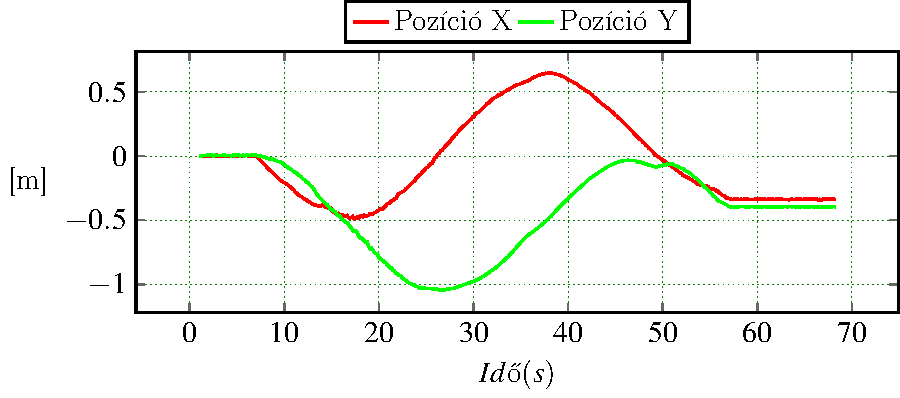
\includegraphics[scale=0.8]{tikz/Left0Right50a.pdf}
  	\end{center}
  \caption{$SSMR-4W$ típusú robot pozíciója, X és Y tengelyekre bontva, keréksebességek BL=FL=0 és a FR=BR= 50\degree/s}
    \label{fig:Left0Right50a}
\end{figure}


\begin{figure}[H]
	\begin{center}
  		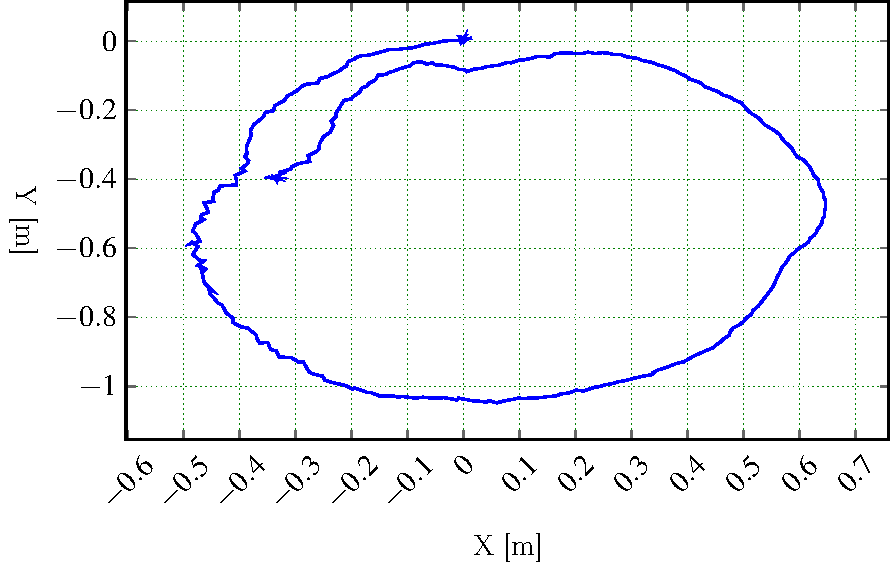
\includegraphics[scale=1]{tikz/Left0Right50b.pdf}
  	\end{center}
  \caption{$SSMR-4W$ típusú robot által leírt pálya, kerekesebességek BL=FL=0 és a FR=BR= 50\degree/s}
  \renewcommand{\figlabel}{Left0Right50b}
  \label{fig:Left0Right50b}
\end{figure}

A mérés során a fordulási szögsebesség 9\degree/s látható a \ref{fig:Left0Right50c} ábran. A LIDAR és HectorMap segítségével mért abszolut szögsebesség zajosabb mint a giroszkóp által mért. A LIDAR-al mért szögsebesség előnyösebb mert a zajokat nem kell integrálni ahhoz hogy megkapjuk a szögsebességet a giroszkóppal ellentétben.

A lineáris sebességeket tekintve \ref{fig:Left0Right50d} szinuszosan változnak, az X és Y tengelyeken, megfigyelhető egy 90\degree eltolódás az X és Y tengelyeken mért szinuszos mozgásban. A kerületi sebesség 0.1 m/s körül adható meg.

\begin{figure}[H]
	\begin{center}
  		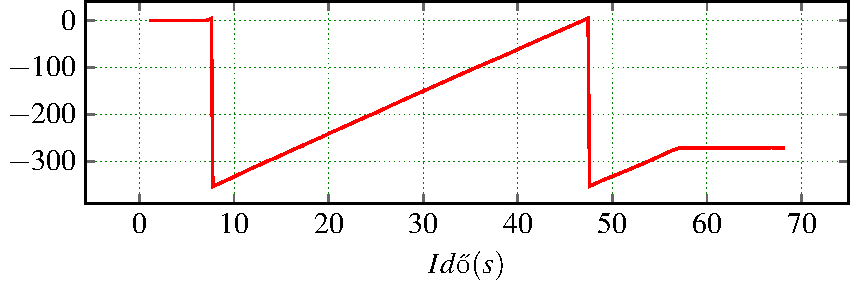
\includegraphics[scale=1]{tikz/Left0Right50c.pdf}
  	\end{center}
  \caption{$SSMR-4W$ típusú robot orientációja,ha a kerékszögsebességek BL=FL=0 és a FR=BR=50\degree/s}
  \label{fig:Left0Right50c}
\end{figure}


\begin{figure}[H]
	\begin{center}
  		\label{fig:Left0Right50d}
  		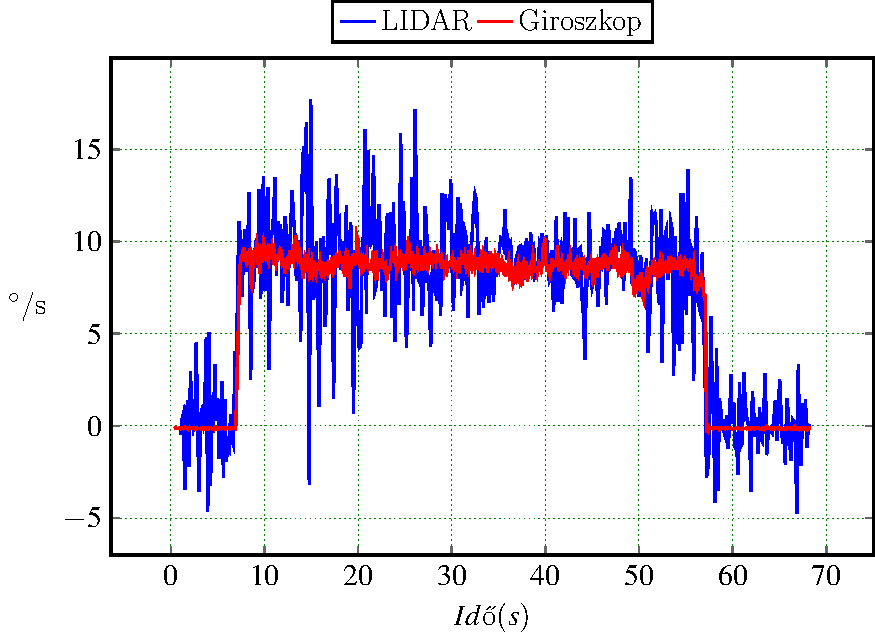
\includegraphics[scale=0.9]{tikz/Left0Right50d.pdf}
  	\end{center}
  \caption{$SSMR-4W$ típusú robot fordulási szögsebessége Giroszkóp és LIDAR által mért értékek, ha a kerékszögsebességek BL=FL=0 és a FR=BR= 50\degree/s}
  \label{fig:Left0Right50d}
\end{figure}


\begin{figure}[H]
	\begin{center}
  		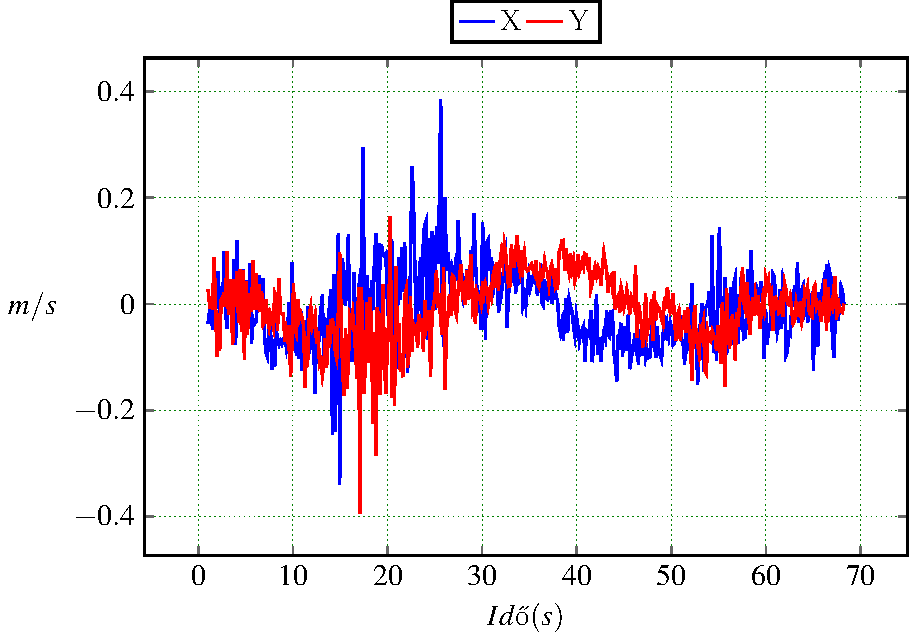
\includegraphics[scale=0.9]{tikz/Left0Right50e.pdf}
    \end{center}
  \caption{$SSMR-4W$ típusú robot súlypontjának sebessége a globális VNR-ben, X és Y tengelyekre bontva, ha a kerékszögsebességek BL=FL=0 és a FR=BR= 50\degree/s}
  \label{fig:Left0Right50e}  
\end{figure}











\subsection{Kavicsos talajon helyben forgás}
A \ref{fig:Left_n50Right50a} megfigyelhető amint a robot kavicsos talajon differenciálisan fordul 60 másodpercen keresztül, ezalatt háromszor teljen korbefordul. A palyat tekintve letrejon egy oldaliranyu mozgás is igy 0.4m kerul odebb. Az oldaliranyu mozgas a nem egyenlo surlodasok es eroeloszlasok miatt jon letre.

\renewcommand{\nth}{2}
\renewcommand{\GlobalPath}{Meresek/Mozgasok/NormalMukodes/DiferencialisanHelybeKavicsos/}
\renewcommand{\secondImage}{*}



\begin{figure}[H]
  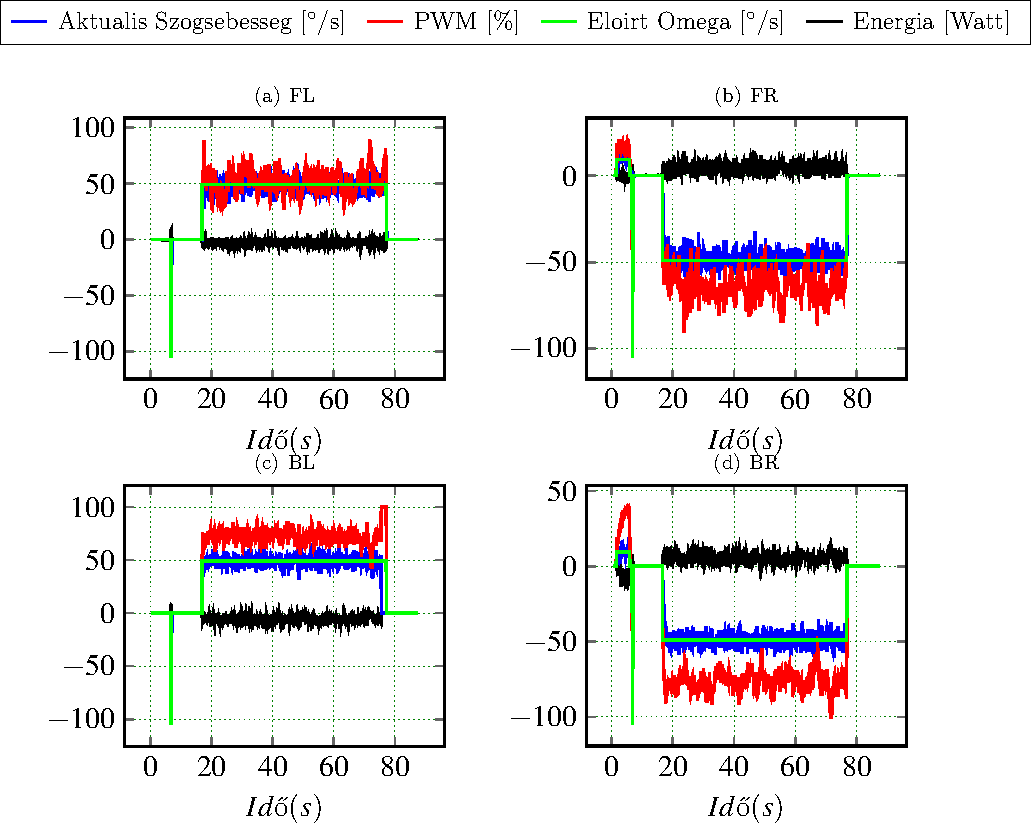
\includegraphics{tikz/Left_n50Right50x.pdf}
  \caption{$SSMR-4W$ típusú robot mozgása, tengelyekre bontva, kereksebessegek BL=FL=0 es a FR=BR= 50\degree/s}
  \label{fig:Left_n50Right50x}
\end{figure}


\begin{figure}[H]
  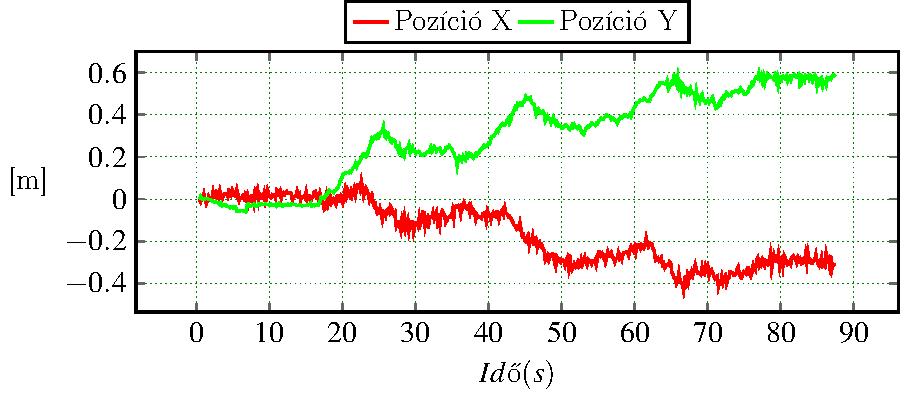
\includegraphics{tikz/Left_n50Right50a.pdf}
  \caption{$SSMR-4W$ típusú robot mozgása, tengelyekre bontva, kereksebessegek BL=FL=-50 es a FR=BR= 50\degree/s}
  \label{fig:Left_n50Right50a}
\end{figure}


\begin{figure}[H]
  \label{fig:Left_n50Right50b}
  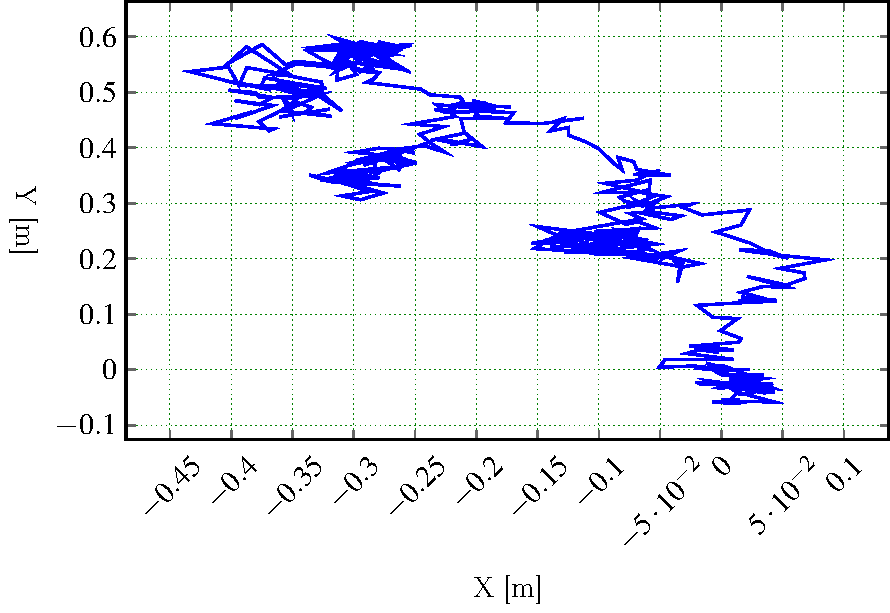
\includegraphics{tikz/Left_n50Right50b.pdf}
  \caption{$SSMR-4W$ típusú robot altal leirt palya, kereksebessegek BL=FL=-50 es a FR=BR= 50\degree/s}
\end{figure}



\begin{figure}[H]
  \label{fig:Left_n50Right50c}
  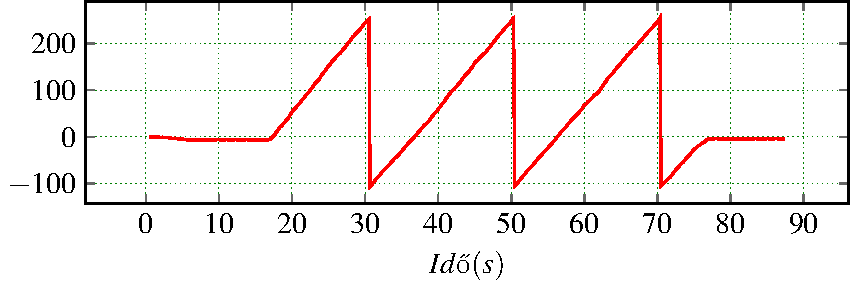
\includegraphics{tikz/Left_n50Right50c.pdf}
  \caption{$SSMR-4W$ típusú robot orientacioja, kereksebessegek BL=FL=-50 es a FR=BR= 50\degree/s}
\end{figure}


\begin{figure}[H]
  \label{fig:Left_n50Right50d}
  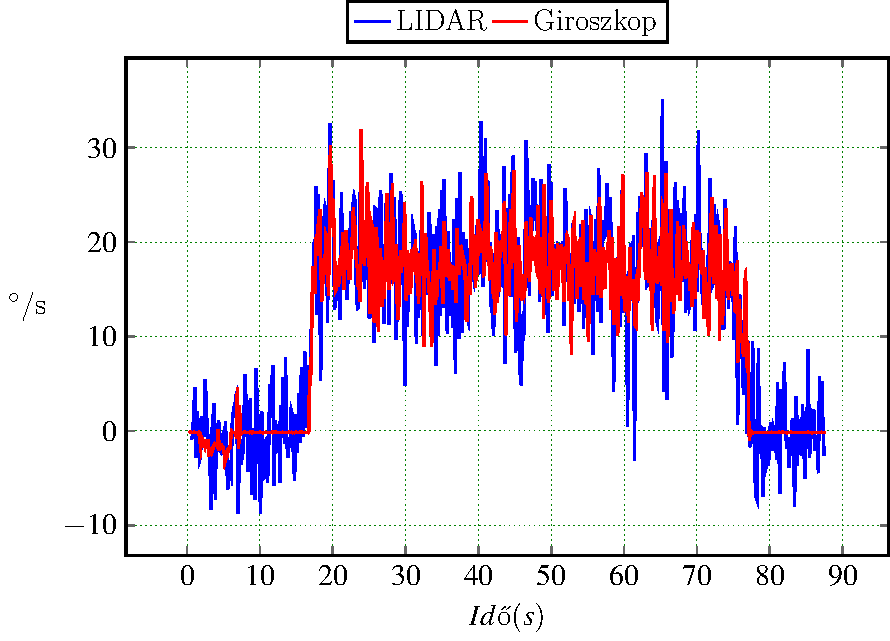
\includegraphics{tikz/Left_n50Right50d.pdf}
  \caption{$SSMR-4W$ típusú robot fordulasi szogsebessege, kereksebessegek BL=FL=-50 es a FR=BR= 50\degree/s}
\end{figure}











\subsection{Kavicsos talajon korpalyan mozgas}


\subsection{Kavicsos talajon korpalyan 50/15}
A \ref{fig:KorP0705a} megfigyelhető amint a robot kavicsos talajon differenciálisan fordul 80 másodpercen keresztül, ezalatt másfélszer körbefordul.

\renewcommand{\GlobalPath}{Meresek/Mozgasok/NormalMukodes/Korpalya_07_05_Kavicsos/}
\renewcommand{\secondImage}{*}

%kep a talajrol
%

\renewcommand{\sources}{}
\renewcommand{\captionn}{Kep a felszinrol}
\renewcommand{\figlabel}{figm}


\begin{kep}
    \begin{figure}[H]%
    \begin{center}
    
    \subfloat[label a]{
        {\includegraphics[width=9cm]{\mand{\GlobalPath}{talaj1.jpg}} }
        \label{fig:ex3-a}
    }%
    
    \ifthenelse{\equal{\secondImage}{*}}
    {}
    {
        \qquad
        \subfloat[label b]{{\includegraphics[width=9cm]{\mand{\GlobalPath}{talaj1.jpg}} }}%
    }
  
    \label{fig:example}%
    \end{center}
\end{figure}
\end{kep}

\renewcommand{\secondImage}{*}



%1
% %1
    \begin{figure}
    
        %-------------------------------------------------Joint Adatok---------------
        \begin{subfigure}{\textwidth}
            \begin{center}
        
            \input{\mand{\GlobalPath}{L.tex}}
            \pgfplotstableread{NodeLeft.dat}{\leftNode}

            
            \input{\mand{\GlobalPath}{R.tex}}
            \pgfplotstableread{NodeRight.dat}{\rightNode}

        
            \begin{tikzpicture}
            \pgfplotsset{every axis plot/.append style={very thick}}
            \setcaptionsubtype
            
            % megjelenites beallitasai
            
            \begin{groupplot}[%
                        ,group style={%
                            ,group name=my plots
                            ,group size=2 by 2
                            ,vertical sep=1.8cm,
                            ,horizontal sep = 2.4cm,
                            ,ylabels at=edge left
                        }
                        ,width=7cm
                        ,height=6cm
                        ,try min ticks=5
                        ,xlabel={\bfseries{\emph{\idoFelirat}}}
                        ,zlabel={\bfseries{\emph{kg}}}
                        %%ha kell y felirat az elso ketore
                        %,ylabel={\bfseries{\degree$/s$}}
                        %,ylabel style={rotate=-90}
                        %,xtick={0,10,...,60},
                        %,minor tick num=5
                        %,xtick distance=10
                        %,ytick distance=25
                        ,grid=major%both
                        ,every both grid/.style={gray, opacity=0.7},
                        view={0}{90},
                        legend columns=2,
                        %xmin=0,xmax=0.65,
                        %ymin=0,ymax=0.65,
                       % zmin=-5,zmax=60,
                        ]
            %% ide jonnek a adatok. 
            
            %ha kell felirat be kell teni a nextplot[] parameterei koze
            % \nextgroupplot[ylabel=\degree$/s$, ylabel style={rotate=-90},legend to name={CommonLegend},legend style={legend columns=2}]
            \nextgroupplot[]
                \addplot [color=green,each nth point={\nth}] table [header=true, x=Time, y=refOmegaA] {\leftNode};\label{plots:plot3}
                \addplot [color=black,each nth point={\nth}] table [header=true, x=Time, y=effortA] {\leftNode};\label{plots:plot4}
                \addplot [color=blue,each nth point={\nth}] table [header=true, x=Time, y=omegaA] {\leftNode}; \label{plots:plot1}
                \addplot [color=red,each nth point={\nth}] table [header=true, x=Time, y=pwmA] {\leftNode};\label{plots:plot2}
                \coordinate (top) at (rel axis cs:0,1);% coordinate at top of the first plot
            
            \nextgroupplot[]
                \addplot [color=green,each nth point={\nth}] table [header=true, x=Time, y=refOmegaA] {\rightNode};
                \addplot [color=black,each nth point={\nth}] table [header=true, x=Time, y=effortA] {\rightNode};
                \addplot [color=blue,each nth point={\nth}] table [header=true, x=Time, y=omegaA] {\rightNode};
                \addplot [color=red,each nth point={\nth}] table [header=true, x=Time, y=pwmA] {\rightNode};
                    
            \nextgroupplot[]
                \addplot [color=green,each nth point={\nth}] table [header=true, x=Time, y=refOmegaB] {\leftNode};
                \addplot [color=black,each nth point={\nth}] table [header=true, x=Time, y=effortB] {\leftNode};
                \addplot [color=blue,each nth point={\nth}] table [header=true, x=Time, y=omegaB] {\leftNode};
                \addplot [color=red,each nth point={\nth}] table [header=true, x=Time, y=pwmB] {\leftNode};
                   
            \nextgroupplot[]
                \addplot [color=green,each nth point={\nth}] table [header=true, x=Time, y=refOmegaB] {\rightNode};
                \addplot [color=black,each nth point={\nth}] table [header=true, x=Time, y=effortB] {\rightNode};
                \addplot [color=blue,each nth point={\nth}] table [header=true, x=Time, y=omegaB] {\rightNode};
                \addplot [color=red,each nth point={\nth}] table [header=true, x=Time, y=pwmB] {\rightNode};
                \coordinate (bot) at (rel axis cs:1,0);% coordinate at bottom of the last plot
            \end{groupplot}
            
            %\path [nodes={anchor=south,rotate=90,font=\large\bfseries,midway}]
            %  (my plots c1r1.outer north west)--(my plots c1r2.outer south west)
            %    node {Testing of Parameters 1}
            %  (my plots c2r1.outer north west)--(my plots c2r2.outer south west)
            %    node {Testing of Parameters 2};
            
            % legend
            \node[text width=.5\linewidth,align=center,anchor=south] at (my plots c1r1.north) {\caption[]{FL\label{subplot:one}}};
            \node[text width=.5\linewidth,align=center,anchor=south] at (my plots c2r1.north) {\caption[]{FR\label{subplot:two}}};
            \node[text width=.5\linewidth,align=center,anchor=south] at (my plots c1r2.north) {\caption[]{BL\label{subplot:three}}};
            \node[text width=.5\linewidth,align=center,anchor=south] at (my plots c2r2.north) {\caption[]{BR\label{subplot:four}}};
            
            %\path (top-|current bounding box.west)-- 
            %      node[anchor=south,rotate=90] {throughput} 
            %      (bot-|current bounding box.west);
            % legend
            \path (top|-current bounding box.north)--
                  coordinate(legendpos)
                  (bot|-current bounding box.north);
            \matrix[
                matrix of nodes,
                anchor=south,
                draw,
                inner sep=0.2em,
                draw
              ]at([yshift=1ex]legendpos)
              {
                \ref{plots:plot1}& Aktualis Szogsebesseg [\degree$/s$]&[5pt]
                \ref{plots:plot2}& PWM [$\%$] &[5pt]
                \ref{plots:plot3}& Eloirt Omega [\degree$/s]$
                \ref{plots:plot4}& Energia $[Watt]$ &[5pt]\\
            };
           % \centering
            \end{tikzpicture}
            \end{center}
        \end{subfigure}
        
        \iffalse
        %-------------------------------------------------Power Adatok---------------
        \newline
        \begin{subfigure}{\textwidth}
        \begin{center}
        \input{\mand{\GlobalPath}{Power.tex}}
        \pgfplotstableread{Power.dat}{\power}
        
        
        \begin{tikzpicture}
        \pgfplotsset{every axis plot/.append style={very thick}}
        \setcaptionsubtype
        
        % megjelenites beallitasai
        
        \begin{groupplot}[%
                    ,group style={%
                        ,group name=my plots
                        ,group size=1 by 1
                        ,vertical sep=2cm,
                        ,horizontal sep = 0cm,
                        ,ylabels at=edge left
                    }
                    ,width=14.5cm
                    ,height=6cm
                    ,try min ticks=5
                    ,xlabel={\bfseries{\emph{\idoFelirat}}}
                    %,ylabel={\bfseries{\emph{A}}}
                    %,zlabel={\bfseries{\emph{kg}}}
                    ,grid=both
                    ,every both grid/.style={gray, opacity=0.5}
                    ,view={0}{90},
                    %,xtick distance=10
                    %,minor tick num=5
                    %,ytick distance=5
                    %xmin=0,xmax=0.65,
                    %ymin=0,ymax=0.65,
                    %zmin=-5,zmax=60,
                    ]
        %% ide jonnek a adatok.            
                    
        \nextgroupplot[ylabel=\emph{}, ylabel style={rotate=-90}]
         \addplot [color=red,each nth point={\nth}] table [header=true, x=Time, y=voltage] {\power};\label{plots:plot11}
         \addplot [color=green,each nth point={\nth}] table [header=true, x=Time, y=current]{\power};\label{plots:plot12}
         \addplot [color=black,each nth point={\nth}] table [header=true, x=Time, y=power] {\power};\label{plots:plot13}
        \end{groupplot}
        
        %\path [nodes={anchor=south,rotate=90,font=\large\bfseries,midway}]
        %  (my plots c1r1.outer north west)--(my plots c1r2.outer south west)
        %    node {Testing of Parameters 1}
        %  (my plots c2r1.outer north west)--(my plots c2r2.outer south west)
        %    node {Testing of Parameters 2};
        
        % legend
        \node[text width=.5\linewidth,align=center,anchor=south] at (my plots c1r1.north) {\caption[]{Energia Fogyasztas\label{subplot:one}}};
        
        %\path (top-|current bounding box.west)-- 
            %      node[anchor=south,rotate=90] {throughput} 
            %      (bot-|current bounding box.west);
            % legend
            \path (top|-current bounding box.north)--
                  coordinate(legendpos)
                  (bot|-current bounding box.north);
            \matrix[
                matrix of nodes,
                anchor=south,
                draw,
                inner sep=0.2em,
                draw
              ]at([yshift=1ex]legendpos)
              {
                \ref{plots:plot11}&  Akumlator Feszultsege [V]&[5pt]
                \ref{plots:plot12}& Akkumlator Arama [A] &[5pt]
                \ref{plots:plot13}& Teljesitmeny [W] \\
            };
        
        %\centering
        \end{tikzpicture}
        \end{center}
        \end{subfigure}
        % Caption
        %\caption[]{$SSMR-4W$ tipusu robot kereknyomoerok kerekenkeni változása a sulypont fuggvenyeben}\label{abserror}
        \fi
    \end{figure}

\begin{figure}[H]
  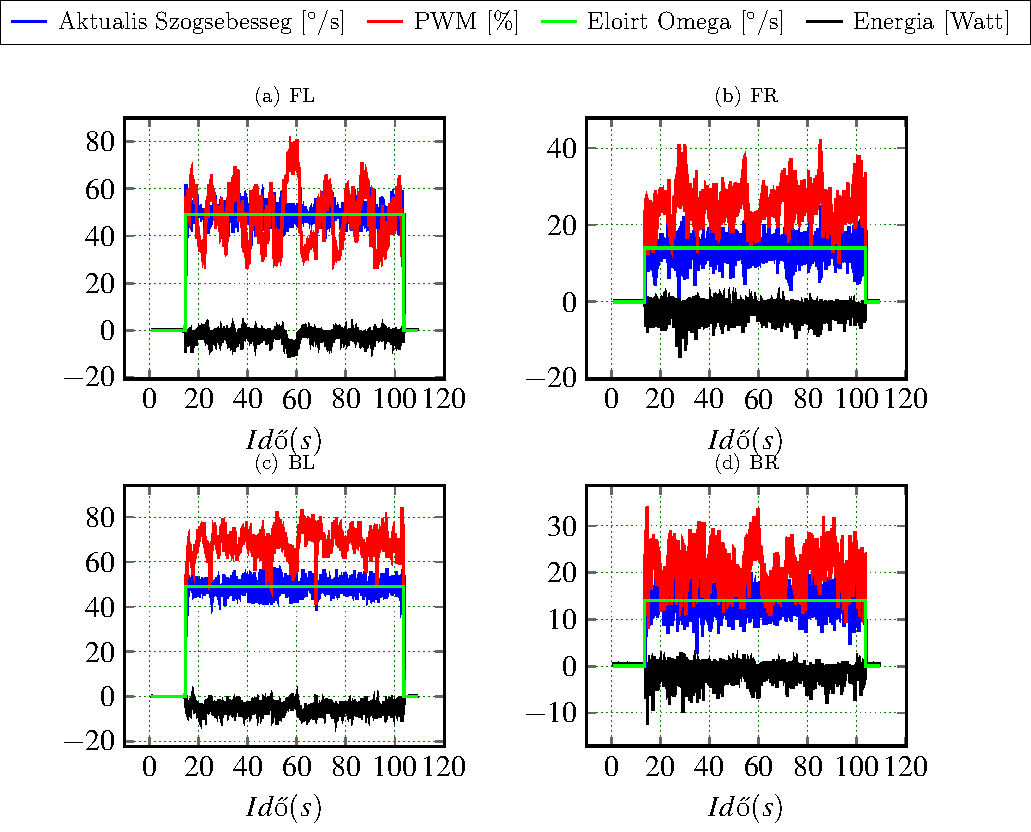
\includegraphics{tikz/KorP0705x.pdf}
  \caption{$SSMR-4W$ típusú robot mozgása, tengelyekre bontva, keréksebességek BL=FL=50\degree/s és a FR=BR=15\degree/s}
  \label{fig:KorP0705x}  
\end{figure}


\begin{figure}[H]
  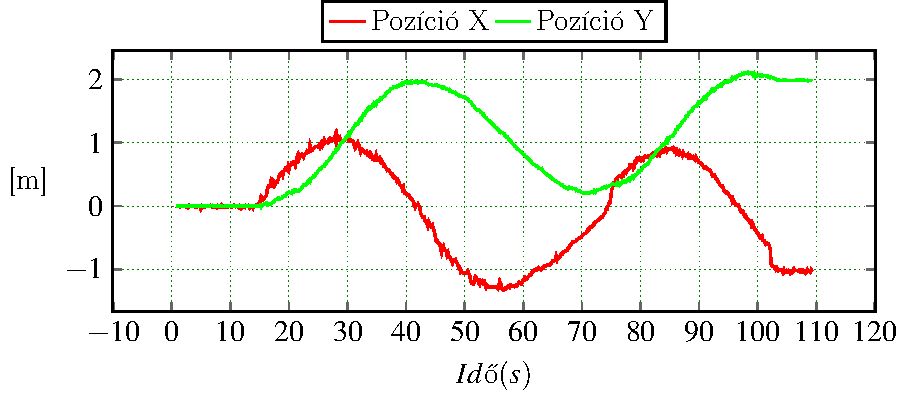
\includegraphics{tikz/KorP0705a.pdf}
  \caption{$SSMR-4W$ típusú robot mozgása, tengelyekre bontva, kerekszögsebességek BL=FL=50\degree/s és a FR=BR=15\degree/s}
  \label{fig:KorP0705a}  
\end{figure}


\begin{figure}[H]
  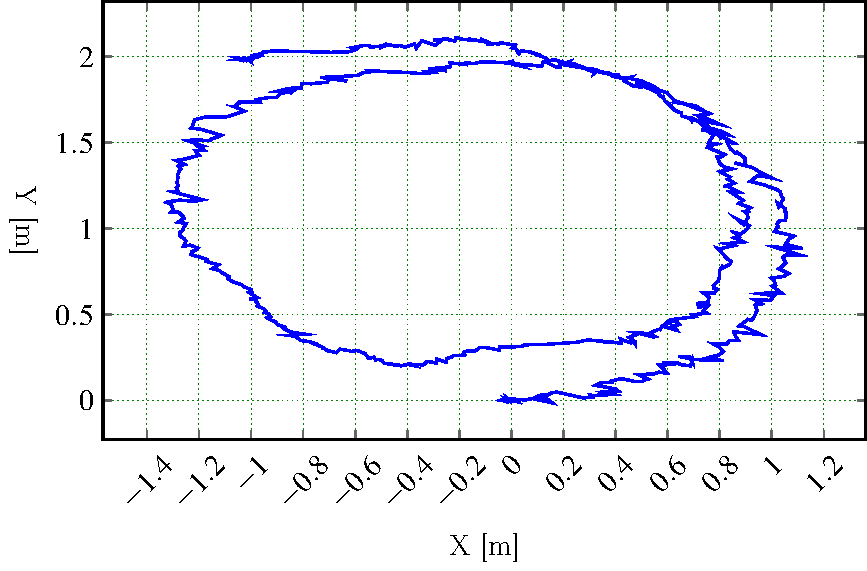
\includegraphics{tikz/KorP0705b.pdf}
  \caption{$SSMR-4W$ típusú robot altal leirt palya, kerekszögsebességek BL=FL=50\degree/s és a FR=BR=15\degree/s}
  \label{fig:KorP0705b}
\end{figure}

A körpalyán mozgás során a robot eltér a szabályos körtöl, és  látható a \ref{fig:KorP0705b} ábrán. A mérések nyilthurokan törének, nincs szabályzókör a pozicióra és a sebességkre.
A szögsebességet tekintve a robot 7\degree/s szögsebességet generál.


%\begin{figure}[H]
%  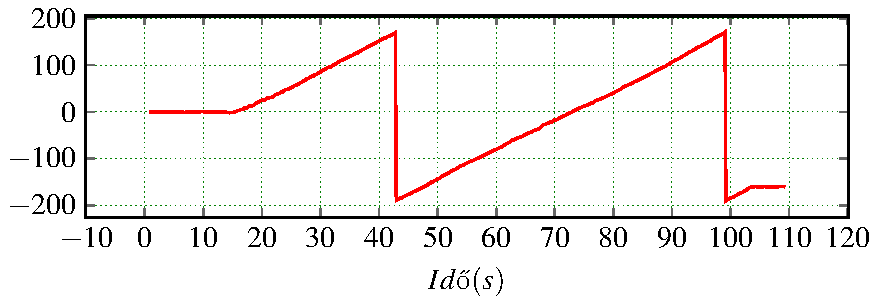
\includegraphics{tikz/KorP0705c.pdf}
%  \caption{$SSMR-4W$ típusú robot orientacioja, kerekszögsebességek %BL=FL=50\degree/s és a FR=BR=15\degree/s}
%  \label{fig:KorP0705c}
%\end{figure}


\begin{figure}[H]
\begin{center}
  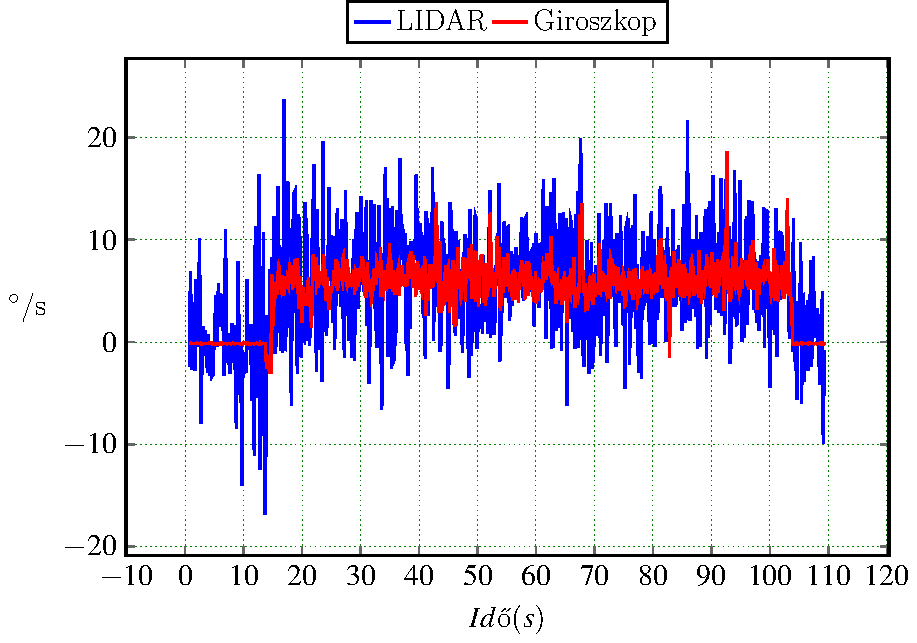
\includegraphics[scale=0.8]{tikz/KorP0705d.pdf}
\end{center}
  \caption{$SSMR-4W$ típusú robot fordulasi szögsebessége, kerekszögsebességek BL=FL=50\degree/s és a FR=BR=15\degree/s}
  \label{fig:KorP0705d}
\end{figure}


\begin{figure}[H]
\begin{center}
  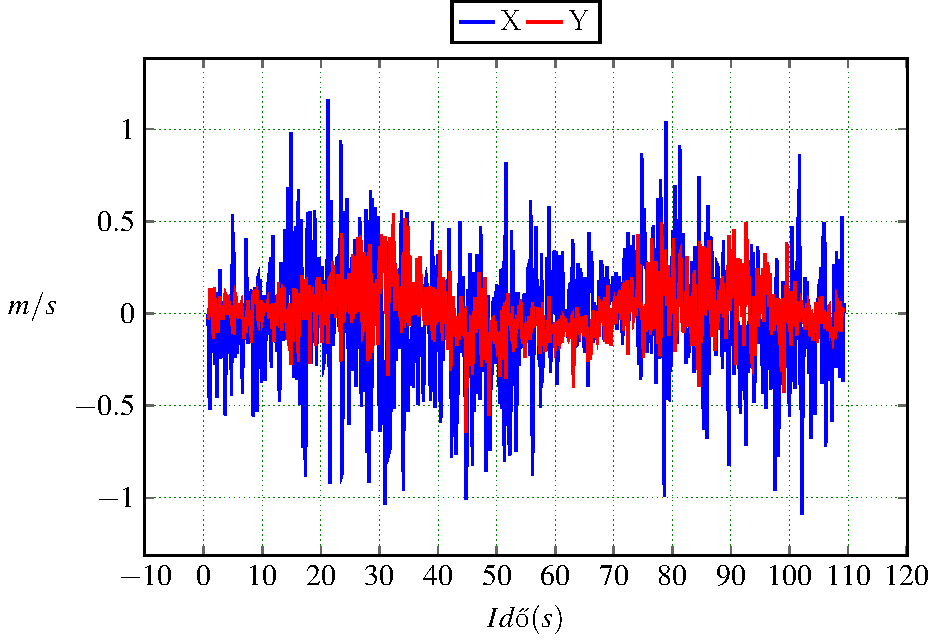
\includegraphics[scale=0.8]{tikz/KorP0705e.pdf}
\end{center}
  \caption{$SSMR-4W$ típusú robot egyenesvonalú sebességei, kerekszögsebességek BL=FL=50\degree/s és a FR=BR=15\degree/s}
  \label{fig:KorP0705e}
\end{figure}

A robot sebességét tekintve a \ref{fig:KorP0705e} látható hogy szinuszosan változuk a pozicióhoz hasonlóan,a robot kiss sebességü mozgása miatt a mérés zajos.
;
\subsection{Kavicsos talajon körpályán 50/25}

Az alábbi méréseknél 80-90s között a robot jobboldali kerekeit vezérlő H-híd túlmelegedése miatt a beléjük épített védelmi funkciónak köszönhetően leálltak így a jobboldali kerek leblokkoltak, így a mozgás pályája is megváltozott.


\renewcommand{\GlobalPath}{Meresek/Mozgasok/NormalMukodes/Korpalya_07_03_Kavicsos/}
\renewcommand{\secondImage}{*}

%kep a talajrol
%

\renewcommand{\sources}{}
\renewcommand{\captionn}{Kep a felszinrol}
\renewcommand{\figlabel}{figm}


\begin{kep}
    \begin{figure}[H]%
    \begin{center}
    
    \subfloat[label a]{
        {\includegraphics[width=9cm]{\mand{\GlobalPath}{talaj1.jpg}} }
        \label{fig:ex3-a}
    }%
    
    \ifthenelse{\equal{\secondImage}{*}}
    {}
    {
        \qquad
        \subfloat[label b]{{\includegraphics[width=9cm]{\mand{\GlobalPath}{talaj1.jpg}} }}%
    }
  
    \label{fig:example}%
    \end{center}
\end{figure}
\end{kep}

\renewcommand{\secondImage}{*}



%1
% %1
    \begin{figure}
    
        %-------------------------------------------------Joint Adatok---------------
        \begin{subfigure}{\textwidth}
            \begin{center}
        
            \input{\mand{\GlobalPath}{L.tex}}
            \pgfplotstableread{NodeLeft.dat}{\leftNode}

            
            \input{\mand{\GlobalPath}{R.tex}}
            \pgfplotstableread{NodeRight.dat}{\rightNode}

        
            \begin{tikzpicture}
            \pgfplotsset{every axis plot/.append style={very thick}}
            \setcaptionsubtype
            
            % megjelenites beallitasai
            
            \begin{groupplot}[%
                        ,group style={%
                            ,group name=my plots
                            ,group size=2 by 2
                            ,vertical sep=1.8cm,
                            ,horizontal sep = 2.4cm,
                            ,ylabels at=edge left
                        }
                        ,width=7cm
                        ,height=6cm
                        ,try min ticks=5
                        ,xlabel={\bfseries{\emph{\idoFelirat}}}
                        ,zlabel={\bfseries{\emph{kg}}}
                        %%ha kell y felirat az elso ketore
                        %,ylabel={\bfseries{\degree$/s$}}
                        %,ylabel style={rotate=-90}
                        %,xtick={0,10,...,60},
                        %,minor tick num=5
                        %,xtick distance=10
                        %,ytick distance=25
                        ,grid=major%both
                        ,every both grid/.style={gray, opacity=0.7},
                        view={0}{90},
                        legend columns=2,
                        %xmin=0,xmax=0.65,
                        %ymin=0,ymax=0.65,
                       % zmin=-5,zmax=60,
                        ]
            %% ide jonnek a adatok. 
            
            %ha kell felirat be kell teni a nextplot[] parameterei koze
            % \nextgroupplot[ylabel=\degree$/s$, ylabel style={rotate=-90},legend to name={CommonLegend},legend style={legend columns=2}]
            \nextgroupplot[]
                \addplot [color=green,each nth point={\nth}] table [header=true, x=Time, y=refOmegaA] {\leftNode};\label{plots:plot3}
                \addplot [color=black,each nth point={\nth}] table [header=true, x=Time, y=effortA] {\leftNode};\label{plots:plot4}
                \addplot [color=blue,each nth point={\nth}] table [header=true, x=Time, y=omegaA] {\leftNode}; \label{plots:plot1}
                \addplot [color=red,each nth point={\nth}] table [header=true, x=Time, y=pwmA] {\leftNode};\label{plots:plot2}
                \coordinate (top) at (rel axis cs:0,1);% coordinate at top of the first plot
            
            \nextgroupplot[]
                \addplot [color=green,each nth point={\nth}] table [header=true, x=Time, y=refOmegaA] {\rightNode};
                \addplot [color=black,each nth point={\nth}] table [header=true, x=Time, y=effortA] {\rightNode};
                \addplot [color=blue,each nth point={\nth}] table [header=true, x=Time, y=omegaA] {\rightNode};
                \addplot [color=red,each nth point={\nth}] table [header=true, x=Time, y=pwmA] {\rightNode};
                    
            \nextgroupplot[]
                \addplot [color=green,each nth point={\nth}] table [header=true, x=Time, y=refOmegaB] {\leftNode};
                \addplot [color=black,each nth point={\nth}] table [header=true, x=Time, y=effortB] {\leftNode};
                \addplot [color=blue,each nth point={\nth}] table [header=true, x=Time, y=omegaB] {\leftNode};
                \addplot [color=red,each nth point={\nth}] table [header=true, x=Time, y=pwmB] {\leftNode};
                   
            \nextgroupplot[]
                \addplot [color=green,each nth point={\nth}] table [header=true, x=Time, y=refOmegaB] {\rightNode};
                \addplot [color=black,each nth point={\nth}] table [header=true, x=Time, y=effortB] {\rightNode};
                \addplot [color=blue,each nth point={\nth}] table [header=true, x=Time, y=omegaB] {\rightNode};
                \addplot [color=red,each nth point={\nth}] table [header=true, x=Time, y=pwmB] {\rightNode};
                \coordinate (bot) at (rel axis cs:1,0);% coordinate at bottom of the last plot
            \end{groupplot}
            
            %\path [nodes={anchor=south,rotate=90,font=\large\bfseries,midway}]
            %  (my plots c1r1.outer north west)--(my plots c1r2.outer south west)
            %    node {Testing of Parameters 1}
            %  (my plots c2r1.outer north west)--(my plots c2r2.outer south west)
            %    node {Testing of Parameters 2};
            
            % legend
            \node[text width=.5\linewidth,align=center,anchor=south] at (my plots c1r1.north) {\caption[]{FL\label{subplot:one}}};
            \node[text width=.5\linewidth,align=center,anchor=south] at (my plots c2r1.north) {\caption[]{FR\label{subplot:two}}};
            \node[text width=.5\linewidth,align=center,anchor=south] at (my plots c1r2.north) {\caption[]{BL\label{subplot:three}}};
            \node[text width=.5\linewidth,align=center,anchor=south] at (my plots c2r2.north) {\caption[]{BR\label{subplot:four}}};
            
            %\path (top-|current bounding box.west)-- 
            %      node[anchor=south,rotate=90] {throughput} 
            %      (bot-|current bounding box.west);
            % legend
            \path (top|-current bounding box.north)--
                  coordinate(legendpos)
                  (bot|-current bounding box.north);
            \matrix[
                matrix of nodes,
                anchor=south,
                draw,
                inner sep=0.2em,
                draw
              ]at([yshift=1ex]legendpos)
              {
                \ref{plots:plot1}& Aktualis Szogsebesseg [\degree$/s$]&[5pt]
                \ref{plots:plot2}& PWM [$\%$] &[5pt]
                \ref{plots:plot3}& Eloirt Omega [\degree$/s]$
                \ref{plots:plot4}& Energia $[Watt]$ &[5pt]\\
            };
           % \centering
            \end{tikzpicture}
            \end{center}
        \end{subfigure}
        
        \iffalse
        %-------------------------------------------------Power Adatok---------------
        \newline
        \begin{subfigure}{\textwidth}
        \begin{center}
        \input{\mand{\GlobalPath}{Power.tex}}
        \pgfplotstableread{Power.dat}{\power}
        
        
        \begin{tikzpicture}
        \pgfplotsset{every axis plot/.append style={very thick}}
        \setcaptionsubtype
        
        % megjelenites beallitasai
        
        \begin{groupplot}[%
                    ,group style={%
                        ,group name=my plots
                        ,group size=1 by 1
                        ,vertical sep=2cm,
                        ,horizontal sep = 0cm,
                        ,ylabels at=edge left
                    }
                    ,width=14.5cm
                    ,height=6cm
                    ,try min ticks=5
                    ,xlabel={\bfseries{\emph{\idoFelirat}}}
                    %,ylabel={\bfseries{\emph{A}}}
                    %,zlabel={\bfseries{\emph{kg}}}
                    ,grid=both
                    ,every both grid/.style={gray, opacity=0.5}
                    ,view={0}{90},
                    %,xtick distance=10
                    %,minor tick num=5
                    %,ytick distance=5
                    %xmin=0,xmax=0.65,
                    %ymin=0,ymax=0.65,
                    %zmin=-5,zmax=60,
                    ]
        %% ide jonnek a adatok.            
                    
        \nextgroupplot[ylabel=\emph{}, ylabel style={rotate=-90}]
         \addplot [color=red,each nth point={\nth}] table [header=true, x=Time, y=voltage] {\power};\label{plots:plot11}
         \addplot [color=green,each nth point={\nth}] table [header=true, x=Time, y=current]{\power};\label{plots:plot12}
         \addplot [color=black,each nth point={\nth}] table [header=true, x=Time, y=power] {\power};\label{plots:plot13}
        \end{groupplot}
        
        %\path [nodes={anchor=south,rotate=90,font=\large\bfseries,midway}]
        %  (my plots c1r1.outer north west)--(my plots c1r2.outer south west)
        %    node {Testing of Parameters 1}
        %  (my plots c2r1.outer north west)--(my plots c2r2.outer south west)
        %    node {Testing of Parameters 2};
        
        % legend
        \node[text width=.5\linewidth,align=center,anchor=south] at (my plots c1r1.north) {\caption[]{Energia Fogyasztas\label{subplot:one}}};
        
        %\path (top-|current bounding box.west)-- 
            %      node[anchor=south,rotate=90] {throughput} 
            %      (bot-|current bounding box.west);
            % legend
            \path (top|-current bounding box.north)--
                  coordinate(legendpos)
                  (bot|-current bounding box.north);
            \matrix[
                matrix of nodes,
                anchor=south,
                draw,
                inner sep=0.2em,
                draw
              ]at([yshift=1ex]legendpos)
              {
                \ref{plots:plot11}&  Akumlator Feszultsege [V]&[5pt]
                \ref{plots:plot12}& Akkumlator Arama [A] &[5pt]
                \ref{plots:plot13}& Teljesitmeny [W] \\
            };
        
        %\centering
        \end{tikzpicture}
        \end{center}
        \end{subfigure}
        % Caption
        %\caption[]{$SSMR-4W$ tipusu robot kereknyomoerok kerekenkeni változása a sulypont fuggvenyeben}\label{abserror}
        \fi
    \end{figure}



\begin{figure}[H]
  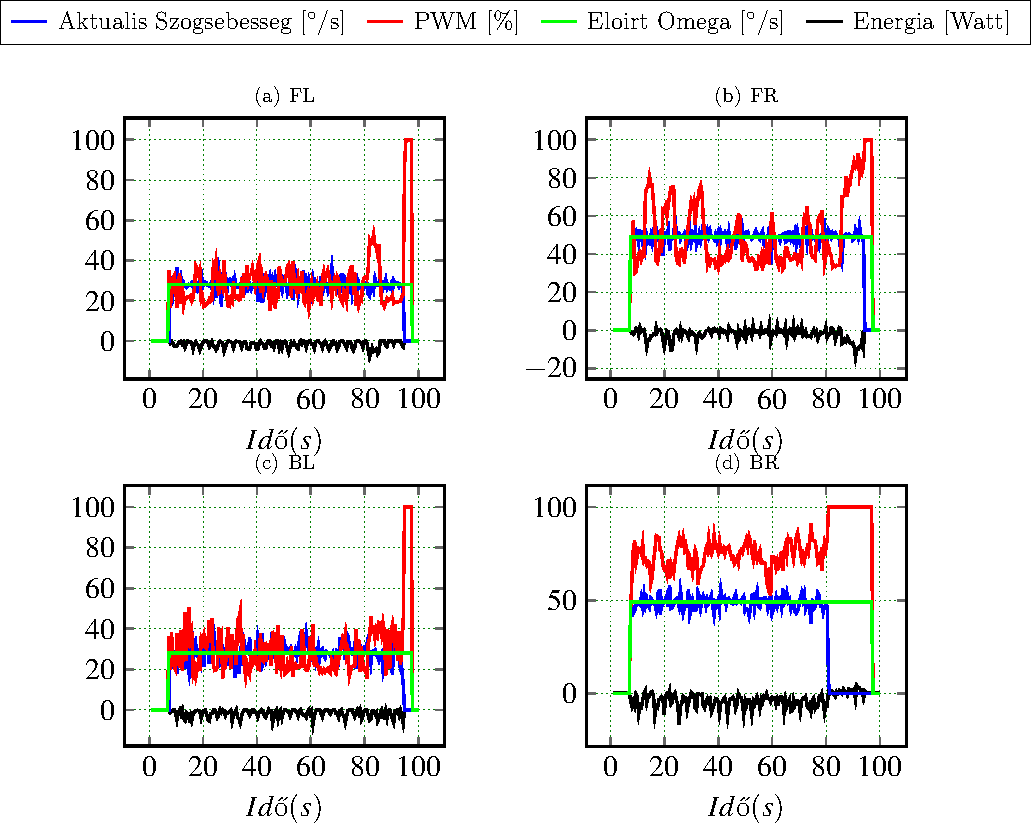
\includegraphics{tikz/KorP0703x.pdf}
  \caption{$SSMR-4W$ típusú robot motorvezérlő jelei, ha kerékszögsebességek BL=FL=25\degree/s és a FR=BR=50\degree/s}
  \label{fig:KorP0703x}
\end{figure}


\begin{figure}[H]
  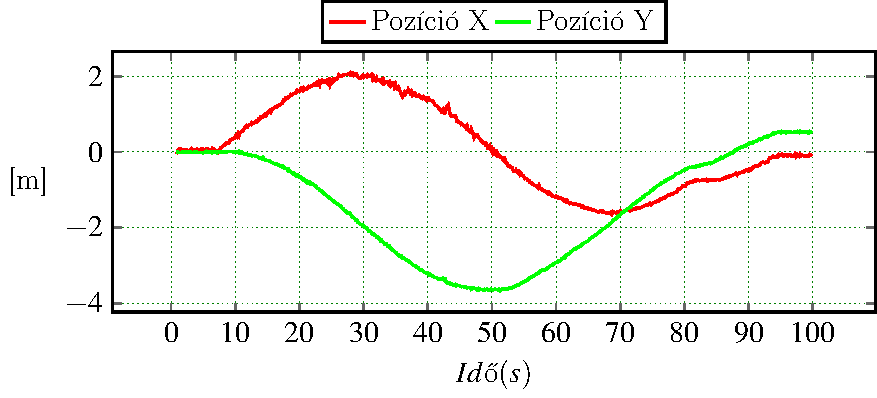
\includegraphics{tikz/KorP0703a.pdf}
  \caption{$SSMR-4W$ típusú robot mozgása, tengelyekre bontva, ha kerékszögsebességek BL=FL=25\degree/s és a FR=BR=50\degree/s }
  \label{fig:KorP0703a}
\end{figure}



\begin{figure}[H]
  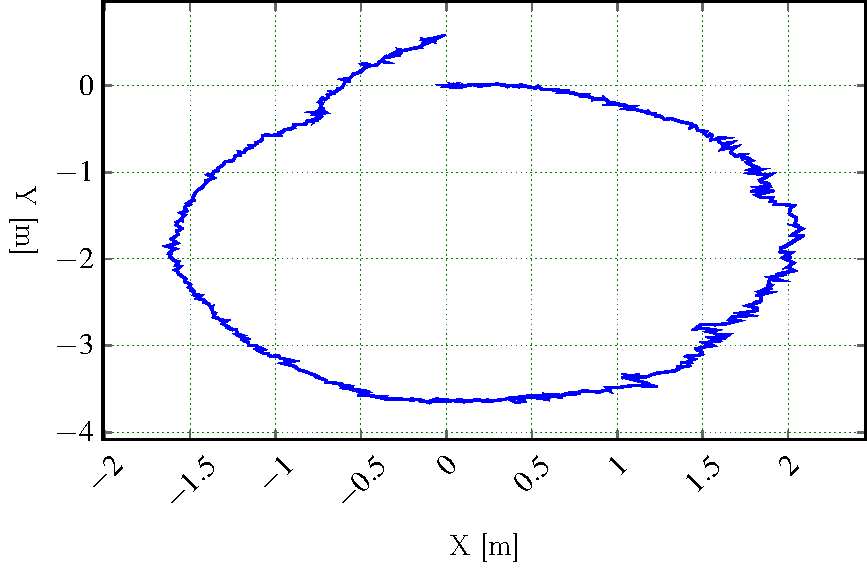
\includegraphics{tikz/KorP0703b.pdf}
  \caption{$SSMR-4W$ típusú robot által leírt pálya, ha kerékszögsebességek BL=FL=25\degree/s és a FR=BR=50\degree/s}
  \label{fig:KorP0703b}
\end{figure}


%\begin{figure}[H]
%  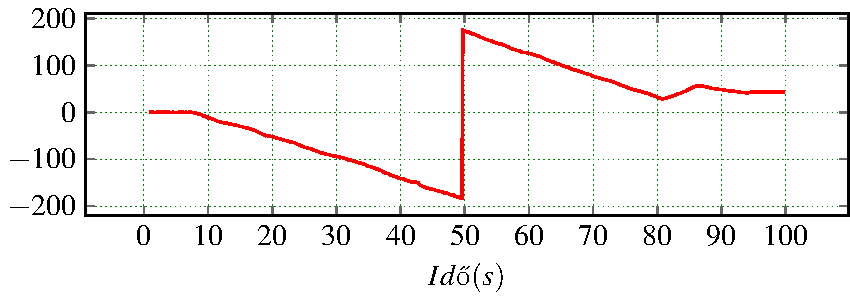
\includegraphics{tikz/KorP0703c.pdf}
%  \caption{$SSMR-4W$ típusú robot orientációja, ha kerékszögsebességek %BL=FL=25\degree/s és a FR=BR=50\degree/s}
%  \label{fig:KorP0703c}
%\end{figure}


\begin{figure}[H]
  \begin{center}
  	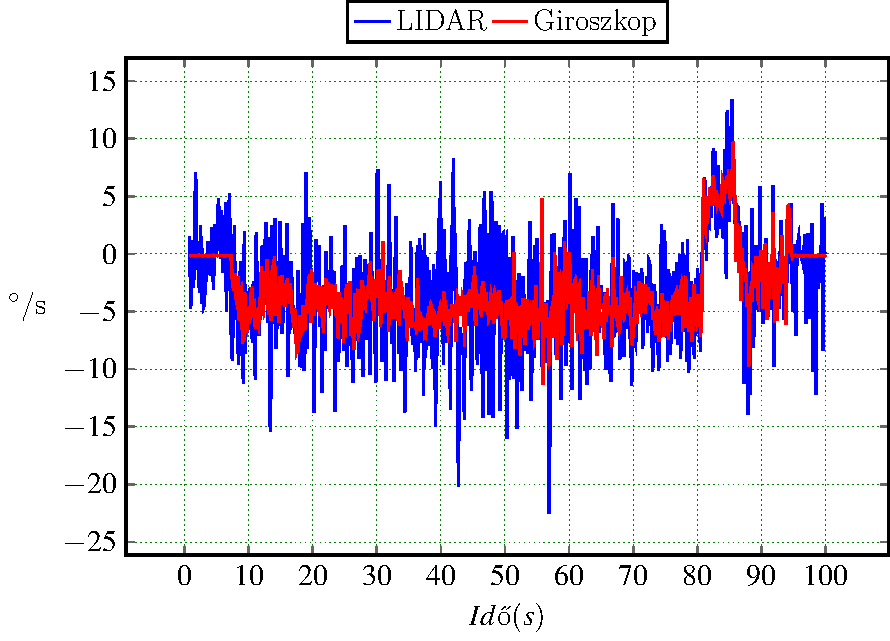
\includegraphics[scale=1]{tikz/KorP0703d.pdf}
  \end{center}
  \caption{$SSMR-4W$ típusú robot fordulási szögsebessége, ha kerékszögsebességek BL=FL=25\degree/s és a FR=BR=50\degree/s}
  \label{fig:KorP0703d}
\end{figure}

%\begin{figure}[H]
%  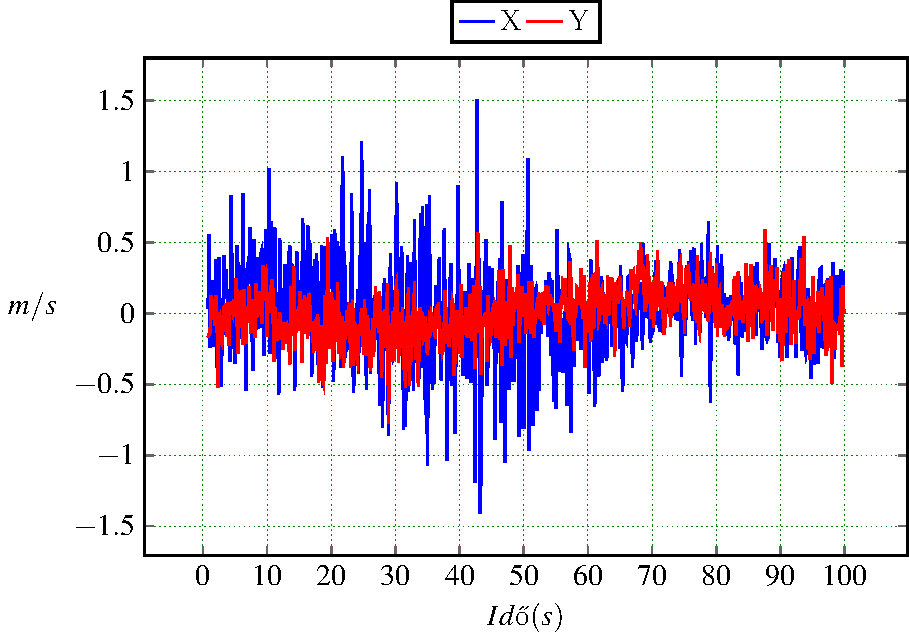
\includegraphics{tikz/KorP0703e.pdf}
%  \caption{$SSMR-4W$ típusú robot egyenesvonalu sebessegei, ha %kerékszögsebességek BL=FL=25\degree/s és a FR=BR=50\degree/s}
%  \label{fig:KorP0703e}
%\end{figure}


;

------------------------------------


\begin{figure}[H]
  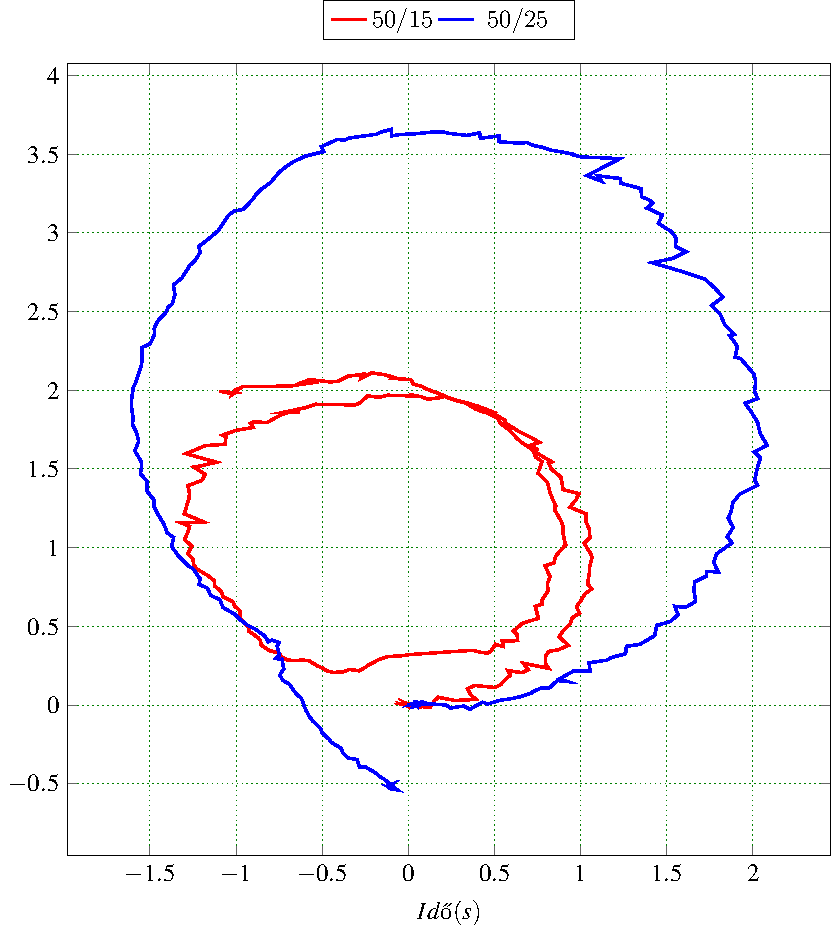
\includegraphics{tikz/KorpalyakKavicsos.pdf}
  \caption{Kulombozo korpalyak}
  \label{fig:KorpalyakKavicsos}  
\end{figure}





\renewcommand{\GlobalPath}{Meresek/Mozgasok/GyergyoFuvesUdvar/M1/}
\renewcommand{\plotRotSpeed}{o}
\renewcommand{\plotSpeed}{o}
%
\subsubsection{Talajon valo mozgas meresi eredmenyei}


\renewcommand{\AbraFelirat}{$SSMR-4W$ tipusu robot kereknyomoerok kerekenkeni változása a sulypont fuggvenyebenddd}

%kep a talajrol


\renewcommand{\sources}{}
\renewcommand{\captionn}{Kep a felszinrol}
\renewcommand{\figlabel}{figm}


\begin{kep}
    \begin{figure}[H]%
    \begin{center}
    
    \subfloat[label a]{
        {\includegraphics[width=9cm]{\mand{\GlobalPath}{talaj1.jpg}} }
        \label{fig:ex3-a}
    }%
    
    \ifthenelse{\equal{\secondImage}{*}}
    {}
    {
        \qquad
        \subfloat[label b]{{\includegraphics[width=9cm]{\mand{\GlobalPath}{talaj1.jpg}} }}%
    }
  
    \label{fig:example}%
    \end{center}
\end{figure}
\end{kep}

\renewcommand{\secondImage}{*}



%1
 %1
    \begin{figure}
    
        %-------------------------------------------------Joint Adatok---------------
        \begin{subfigure}{\textwidth}
            \begin{center}
        
            \input{\mand{\GlobalPath}{L.tex}}
            \pgfplotstableread{NodeLeft.dat}{\leftNode}

            
            \input{\mand{\GlobalPath}{R.tex}}
            \pgfplotstableread{NodeRight.dat}{\rightNode}

        
            \begin{tikzpicture}
            \pgfplotsset{every axis plot/.append style={very thick}}
            \setcaptionsubtype
            
            % megjelenites beallitasai
            
            \begin{groupplot}[%
                        ,group style={%
                            ,group name=my plots
                            ,group size=2 by 2
                            ,vertical sep=1.8cm,
                            ,horizontal sep = 2.4cm,
                            ,ylabels at=edge left
                        }
                        ,width=7cm
                        ,height=6cm
                        ,try min ticks=5
                        ,xlabel={\bfseries{\emph{\idoFelirat}}}
                        ,zlabel={\bfseries{\emph{kg}}}
                        %%ha kell y felirat az elso ketore
                        %,ylabel={\bfseries{\degree$/s$}}
                        %,ylabel style={rotate=-90}
                        %,xtick={0,10,...,60},
                        %,minor tick num=5
                        %,xtick distance=10
                        %,ytick distance=25
                        ,grid=major%both
                        ,every both grid/.style={gray, opacity=0.7},
                        view={0}{90},
                        legend columns=2,
                        %xmin=0,xmax=0.65,
                        %ymin=0,ymax=0.65,
                       % zmin=-5,zmax=60,
                        ]
            %% ide jonnek a adatok. 
            
            %ha kell felirat be kell teni a nextplot[] parameterei koze
            % \nextgroupplot[ylabel=\degree$/s$, ylabel style={rotate=-90},legend to name={CommonLegend},legend style={legend columns=2}]
            \nextgroupplot[]
                \addplot [color=green,each nth point={\nth}] table [header=true, x=Time, y=refOmegaA] {\leftNode};\label{plots:plot3}
                \addplot [color=black,each nth point={\nth}] table [header=true, x=Time, y=effortA] {\leftNode};\label{plots:plot4}
                \addplot [color=blue,each nth point={\nth}] table [header=true, x=Time, y=omegaA] {\leftNode}; \label{plots:plot1}
                \addplot [color=red,each nth point={\nth}] table [header=true, x=Time, y=pwmA] {\leftNode};\label{plots:plot2}
                \coordinate (top) at (rel axis cs:0,1);% coordinate at top of the first plot
            
            \nextgroupplot[]
                \addplot [color=green,each nth point={\nth}] table [header=true, x=Time, y=refOmegaA] {\rightNode};
                \addplot [color=black,each nth point={\nth}] table [header=true, x=Time, y=effortA] {\rightNode};
                \addplot [color=blue,each nth point={\nth}] table [header=true, x=Time, y=omegaA] {\rightNode};
                \addplot [color=red,each nth point={\nth}] table [header=true, x=Time, y=pwmA] {\rightNode};
                    
            \nextgroupplot[]
                \addplot [color=green,each nth point={\nth}] table [header=true, x=Time, y=refOmegaB] {\leftNode};
                \addplot [color=black,each nth point={\nth}] table [header=true, x=Time, y=effortB] {\leftNode};
                \addplot [color=blue,each nth point={\nth}] table [header=true, x=Time, y=omegaB] {\leftNode};
                \addplot [color=red,each nth point={\nth}] table [header=true, x=Time, y=pwmB] {\leftNode};
                   
            \nextgroupplot[]
                \addplot [color=green,each nth point={\nth}] table [header=true, x=Time, y=refOmegaB] {\rightNode};
                \addplot [color=black,each nth point={\nth}] table [header=true, x=Time, y=effortB] {\rightNode};
                \addplot [color=blue,each nth point={\nth}] table [header=true, x=Time, y=omegaB] {\rightNode};
                \addplot [color=red,each nth point={\nth}] table [header=true, x=Time, y=pwmB] {\rightNode};
                \coordinate (bot) at (rel axis cs:1,0);% coordinate at bottom of the last plot
            \end{groupplot}
            
            %\path [nodes={anchor=south,rotate=90,font=\large\bfseries,midway}]
            %  (my plots c1r1.outer north west)--(my plots c1r2.outer south west)
            %    node {Testing of Parameters 1}
            %  (my plots c2r1.outer north west)--(my plots c2r2.outer south west)
            %    node {Testing of Parameters 2};
            
            % legend
            \node[text width=.5\linewidth,align=center,anchor=south] at (my plots c1r1.north) {\caption[]{FL\label{subplot:one}}};
            \node[text width=.5\linewidth,align=center,anchor=south] at (my plots c2r1.north) {\caption[]{FR\label{subplot:two}}};
            \node[text width=.5\linewidth,align=center,anchor=south] at (my plots c1r2.north) {\caption[]{BL\label{subplot:three}}};
            \node[text width=.5\linewidth,align=center,anchor=south] at (my plots c2r2.north) {\caption[]{BR\label{subplot:four}}};
            
            %\path (top-|current bounding box.west)-- 
            %      node[anchor=south,rotate=90] {throughput} 
            %      (bot-|current bounding box.west);
            % legend
            \path (top|-current bounding box.north)--
                  coordinate(legendpos)
                  (bot|-current bounding box.north);
            \matrix[
                matrix of nodes,
                anchor=south,
                draw,
                inner sep=0.2em,
                draw
              ]at([yshift=1ex]legendpos)
              {
                \ref{plots:plot1}& Aktualis Szogsebesseg [\degree$/s$]&[5pt]
                \ref{plots:plot2}& PWM [$\%$] &[5pt]
                \ref{plots:plot3}& Eloirt Omega [\degree$/s]$
                \ref{plots:plot4}& Energia $[Watt]$ &[5pt]\\
            };
           % \centering
            \end{tikzpicture}
            \end{center}
        \end{subfigure}
        
        \iffalse
        %-------------------------------------------------Power Adatok---------------
        \newline
        \begin{subfigure}{\textwidth}
        \begin{center}
        \input{\mand{\GlobalPath}{Power.tex}}
        \pgfplotstableread{Power.dat}{\power}
        
        
        \begin{tikzpicture}
        \pgfplotsset{every axis plot/.append style={very thick}}
        \setcaptionsubtype
        
        % megjelenites beallitasai
        
        \begin{groupplot}[%
                    ,group style={%
                        ,group name=my plots
                        ,group size=1 by 1
                        ,vertical sep=2cm,
                        ,horizontal sep = 0cm,
                        ,ylabels at=edge left
                    }
                    ,width=14.5cm
                    ,height=6cm
                    ,try min ticks=5
                    ,xlabel={\bfseries{\emph{\idoFelirat}}}
                    %,ylabel={\bfseries{\emph{A}}}
                    %,zlabel={\bfseries{\emph{kg}}}
                    ,grid=both
                    ,every both grid/.style={gray, opacity=0.5}
                    ,view={0}{90},
                    %,xtick distance=10
                    %,minor tick num=5
                    %,ytick distance=5
                    %xmin=0,xmax=0.65,
                    %ymin=0,ymax=0.65,
                    %zmin=-5,zmax=60,
                    ]
        %% ide jonnek a adatok.            
                    
        \nextgroupplot[ylabel=\emph{}, ylabel style={rotate=-90}]
         \addplot [color=red,each nth point={\nth}] table [header=true, x=Time, y=voltage] {\power};\label{plots:plot11}
         \addplot [color=green,each nth point={\nth}] table [header=true, x=Time, y=current]{\power};\label{plots:plot12}
         \addplot [color=black,each nth point={\nth}] table [header=true, x=Time, y=power] {\power};\label{plots:plot13}
        \end{groupplot}
        
        %\path [nodes={anchor=south,rotate=90,font=\large\bfseries,midway}]
        %  (my plots c1r1.outer north west)--(my plots c1r2.outer south west)
        %    node {Testing of Parameters 1}
        %  (my plots c2r1.outer north west)--(my plots c2r2.outer south west)
        %    node {Testing of Parameters 2};
        
        % legend
        \node[text width=.5\linewidth,align=center,anchor=south] at (my plots c1r1.north) {\caption[]{Energia Fogyasztas\label{subplot:one}}};
        
        %\path (top-|current bounding box.west)-- 
            %      node[anchor=south,rotate=90] {throughput} 
            %      (bot-|current bounding box.west);
            % legend
            \path (top|-current bounding box.north)--
                  coordinate(legendpos)
                  (bot|-current bounding box.north);
            \matrix[
                matrix of nodes,
                anchor=south,
                draw,
                inner sep=0.2em,
                draw
              ]at([yshift=1ex]legendpos)
              {
                \ref{plots:plot11}&  Akumlator Feszultsege [V]&[5pt]
                \ref{plots:plot12}& Akkumlator Arama [A] &[5pt]
                \ref{plots:plot13}& Teljesitmeny [W] \\
            };
        
        %\centering
        \end{tikzpicture}
        \end{center}
        \end{subfigure}
        % Caption
        %\caption[]{$SSMR-4W$ tipusu robot kereknyomoerok kerekenkeni változása a sulypont fuggvenyeben}\label{abserror}
        \fi
    \end{figure}

%2
    %2
    \begin{figure}[H]
        %\ContinuedFloat
        %-------------------------------------------------Pozicio X es Y Adatok---------------
       % \newline
        \begin{subfigure}{\textwidth}
        \begin{center}
           \input{\mand{\GlobalPath}{Pos.tex}}
            \pgfplotstableread{PositionOrientation.dat}{\pos}
            \centering
            \begin{tikzpicture}
            \pgfplotsset{every axis plot/.append style={very thick}}
            \setcaptionsubtype
            
            % megjelenites beallitasai
            
            \begin{groupplot}[%
                        ,group style={%
                            ,group name=my plots
                            ,group size=1 by 1
                            ,vertical sep=2cm,
                            ,horizontal sep = 0cm,
                            ,ylabels at=edge left
                        }
                        ,width=14.5cm
                        ,height=6cm
                        ,try min ticks=5
                        ,xlabel={\bfseries{\emph{\idoFelirat}}}
                        %,ylabel={\bfseries{\emph{A}}}
                        %,zlabel={\bfseries{\emph{kg}}}
                        ,grid=both
                        ,every both grid/.style={gray, opacity=0.5}
                        ,view={0}{90},
                        %,xtick distance=10
                        %,ytick distance=0.4
                        %,minor tick num=5
                        %xmin=0,xmax=0.65,
                        %ymin=0,ymax=0.65,
                        %zmin=-5,zmax=60,
                        ]
            %% ide jonnek a adatok.            
                        
            \nextgroupplot[ylabel=\emph{m}, ylabel style={rotate=-90}]
             \addplot [color=red,each nth point={\nth}] table [header=true, x=Time, y=poseX] {\pos};\label{plots:plot21}
             %\addlegendentry{Pozíció X [m]} 
             \addplot [color=green,each nth point={\nth}] table [header=true, x=Time, y=poseY]{\pos};\label{plots:plot22}                            %\addlegendentry{Pozíció Y [m]} 
            \end{groupplot}
            
            %\path [nodes={anchor=south,rotate=90,font=\large\bfseries,midway}]
            %  (my plots c1r1.outer north west)--(my plots c1r2.outer south west)
            %    node {Testing of Parameters 1}
            %  (my plots c2r1.outer north west)--(my plots c2r2.outer south west)
            %    node {Testing of Parameters 2};
            
            % legend
            \node[text width=.5\linewidth,align=center,anchor=south] at (my plots c1r1.north) {\caption[]{Robot Pozíció Tengelyekre           \label{subplot:\figlabela}}};
            
            %\path (top-|current bounding box.west)-- 
                %      node[anchor=south,rotate=90] {throughput} 
                %      (bot-|current bounding box.west);
                % legend
                \path (top|-current bounding box.north)--
                      coordinate(legendpos)
                      (bot|-current bounding box.north);
                \matrix[
                    matrix of nodes,
                    anchor=south,
                    draw,
                    inner sep=0.2em,
                    draw
                  ]at([yshift=1ex]legendpos)
                  {
                    \ref{plots:plot21}&Pozíció X [m] &[5pt]
                    \ref{plots:plot22}&Pozíció Y [m] &[5pt]\\
                };
            
            %\centering
            \end{tikzpicture}
            \end{center}
        \end{subfigure}
        
        %-------------------------------------------------Palya Adatok---------------
      %  \newline
        \begin{subfigure}{\textwidth}
           \begin{center}
            \input{\mand{\GlobalPath}{/Pos.tex}}
            \pgfplotstableread{PositionOrientation.dat}{\position}
            
            \begin{tikzpicture}
                \pgfplotsset{every axis plot/.append style={very thick}}
                \setcaptionsubtype
            
                % megjelenites beallitasai
            
                \begin{groupplot}[%
                        ,group style={%
                            ,group name=my plots
                            ,group size=1 by 1
                            ,vertical sep=2cm,
                            ,horizontal sep = 0cm,
                            ,ylabels at=edge left
                        }
                        ,width=14.5cm
                        ,height=9cm
                        %,try min ticks=5
                        ,xlabel={\bfseries{\emph{m}}}
                        ,ylabel={\bfseries{\emph{m}}}
                        ,zlabel={\bfseries{\emph{\idoFelirat}}}
                        ,grid=both
                        ,every both grid/.style={gray, opacity=0.5}
                        ,view={45}{45}
                        %,xtick distance=0.25
                        %,ytick distance=0.25
                        %,minor tick num=5
                        ,xticklabel style={rotate=45},
                        ,ylabel style={rotate=-90}
                        %xmin=0,xmax=0.65,
                        %ymin=0,ymax=0.65,
                       % zmin=-5,zmax=60,
                        ]
                    %% ide jonnek a adatok.            
                                
                    %\nextgroupplot[ylabel=\emph{A}, ylabel style={rotate=-90}]
                    \nextgroupplot[]
                           % \addplot3 []  table [header=true, x=poseX, y=poseY, z=Time] {\position};
                           
                            \addplot [color=blue,each nth point={\nth}] table [header=true, x=poseX, y=poseY] {\position};
                            
                            %\addplot [color=blue] table [header=true, x=poseX, y=poseY] {\position};
                         %%   \addplot[red,quiver={u=u,v=v}] table [header=true, x=poseX, y=poseY, u=poseX, v=poseY] {\position};
        
        
        
        
            \end{groupplot}
            
                %\path [nodes={anchor=south,rotate=90,font=\large\bfseries,midway}]
                %  (my plots c1r1.outer north west)--(my plots c1r2.outer south west)
                %    node {Testing of Parameters 1}
                %  (my plots c2r1.outer north west)--(my plots c2r2.outer south west)
                %    node {Testing of Parameters 2};
                
                % legend
                \node[text width=.5\linewidth,align=center,anchor=south] at (my plots c1r1.north) {\caption[]{Robot Által Leirt Pálya     \label{subplot:\figlabelb}}};
                
                %\centering
            \end{tikzpicture}
            \end{center}
    \end{subfigure}
        
        %-------------------------------------------------Orientacio Adatok---------------
       % \newline
        \begin{subfigure}{\textwidth}
        \begin{center}
        \input{\mand{\GlobalPath}{Pos.tex}}
        \pgfplotstableread{PositionOrientation.dat}{\pos}
        
        \begin{tikzpicture}
        \pgfplotsset{every axis plot/.append style={very thick}}
        \setcaptionsubtype
        
        % megjelenites beallitasai
        
        \begin{groupplot}[%
                    ,group style={%
                        ,group name=my plots
                        ,group size=1 by 1
                        ,vertical sep=2cm,
                        ,horizontal sep = 0cm,
                        ,ylabels at=edge left
                    }
                    ,width=14.5cm
                    ,height=5cm
                    ,try min ticks=5
                    ,xlabel={\bfseries{\emph{\idoFelirat}}}
                    %,ylabel={\bfseries{\emph{A}}}
                    %,zlabel={\bfseries{\emph{kg}}}
                    ,grid=both
                    ,every both grid/.style={gray, opacity=0.5}
                    ,view={0}{90},
                    %,xtick distance=10
                    %,ytick distance=20
                    %,minor tick num=5
                    %xmin=0,xmax=0.65,
                    %ymin=0,ymax=0.65,
                    %zmin=-5,zmax=60,
                    ]
        %% ide jonnek a adatok.            
                    
        \nextgroupplot[ylabel=\emph{$[\degree]$}], ylabel style={rotate=-90}]
        \addplot [color=red,each nth point={\nth}] table [header=true, x=Time, y=orZ] {\pos};\label{plots:plot41}
        \end{groupplot}
        
        %\path [nodes={anchor=south,rotate=90,font=\large\bfseries,midway}]
        %  (my plots c1r1.outer north west)--(my plots c1r2.outer south west)
        %    node {Testing of Parameters 1}
        %  (my plots c2r1.outer north west)--(my plots c2r2.outer south west)
        %    node {Testing of Parameters 2};
        
        % legend
        \node[text width=.5\linewidth,align=center,anchor=south] at (my plots c1r1.north) {\caption[]{Orientáció \label{subplot:\figlabelc}}};
        
        
       % \centering
        \end{tikzpicture}
        \end{center}
        \end{subfigure}
    
        
        % Caption
        \ifthenelse{\equal{\captionn}{*}}
        {}
        {\captionof{figure}{\captionn}}
        \renewcommand{\captionn}{*}
        \label{subplot:\figlabel}
       
    \end{figure}
    
        \renewcommand{\figlabel}{*}
        \renewcommand{\figlabela}{*}
        \renewcommand{\figlabelb}{*}
        \renewcommand{\figlabelc}{*}

%3
%    %3
    \begin{figure}
        %\ContinuedFloat
        \input{\mand{\GlobalPath}{Pos.tex}}
        \ifthenelse{\equal{\plotSpeed}{*}}
        { }
        {
        \newline
        \begin{subfigure}{\textwidth}
            \begin{center}

            \pgfplotstableread{PositionOrientation.dat}{\position}
            
            %-------------------------------------------------Sebesseg Adatok---------------
            \begin{tikzpicture}
                \pgfplotsset{every axis plot/.append style={very thick}}
                \setcaptionsubtype
            
                % megjelenites beallitasai
            
                \begin{groupplot}[%
                        ,group style={%
                            ,group name=my plots
                            ,group size=1 by 1
                            ,vertical sep=2cm,
                            ,horizontal sep = 0cm,
                            ,ylabels at=edge left
                        }
                        ,width=14.5cm
                        ,height=10cm
                        ,try min ticks=5
                        ,ylabel={\bfseries{\emph{$m/s$}}}
                        ,xlabel={\bfseries{\emph{\idoFelirat}}}
                        %,zlabel={\bfseries{\emph{m}}}
                        ,grid=both
                        ,every both grid/.style={gray, opacity=0.5}
                        ,view={0}{90}
                        %,xtick distance=10
                        %,ytick distance=0.1
                        ,ylabel style={rotate=-90}
                        %xmin=0,xmax=0.65,
                        %ymin=0,ymax=0.65,
                       % zmin=-5,zmax=60,
                        ]
                    %% ide jonnek a adatok.            
                                
                    %\nextgroupplot[ylabel=\emph{A}, ylabel style={rotate=-90}]
                    \nextgroupplot[]
                            \addplot [color=blue,each nth point={\nth}] table [header=true, x=Time, y=speedX] {\position}; \label{plots:plot51}
                            \addplot [color=red,each nth point={\nth}] table [header=true, x=Time, y=speedY] {\position}; \label{plots:plot52}
                         %%   \addplot[red,quiver={u=u,v=v}] table [header=true, x=poseX, y=poseY, u=poseX, v=poseY] {\position};
        
        
        
        
            \end{groupplot}
            
                %\path [nodes={anchor=south,rotate=90,font=\large\bfseries,midway}]
                %  (my plots c1r1.outer north west)--(my plots c1r2.outer south west)
                %    node {Testing of Parameters 1}
                %  (my plots c2r1.outer north west)--(my plots c2r2.outer south west)
                %    node {Testing of Parameters 2};
                
                % legend
                \node[text width=.5\linewidth,align=center,anchor=south] at (my plots c1r1.north) {\caption[]{Robot Sebessége a Globális Koordináta Rendszerben
               \label{subplot:\figlabela}}};
                
                      %\path (top-|current bounding box.west)-- 
                %      node[anchor=south,rotate=90] {throughput} 
                %      (bot-|current bounding box.west);
                % legend
                \path (top|-current bounding box.north)--
                      coordinate(legendpos)
                      (bot|-current bounding box.north);
                \matrix[
                    matrix of nodes,
                    anchor=south,
                    draw,
                    inner sep=0.2em,
                    draw
                  ]at([yshift=1ex]legendpos)
                  {
                    \ref{plots:plot51}& Sebesség X &[5pt] 
                    \ref{plots:plot52}& Sebesség Y &[5pt]\\
                  };
                
                %\centering
            \end{tikzpicture}
            \end{center}
        \end{subfigure}
        }
        
        \ifthenelse{\equal{\plotRotSpeed}{*}}
        { }
        { 
        %-------------------------------------------------Fordulasi Sebesseg Adatok---------------
        \newline
        \input{\mand { \GlobalPath}{Pos.tex}}
        \pgfplotstableread{PositionOrientation.dat}{\position}
        
        \input{\mand{\GlobalPath}{ImuA.tex}}
        \pgfplotstableread{ImuA.dat}{\imua}
        
        \begin{subfigure}{\textwidth}
            \begin{center}

            
            \begin{tikzpicture}
                \pgfplotsset{every axis plot/.append style={very thick}}
                \setcaptionsubtype
            
                % megjelenites beallitasai
            
                \begin{groupplot}[%
                        ,group style={%
                            ,group name=my plots
                            ,group size=1 by 1
                            ,vertical sep=2cm,
                            ,horizontal sep = 0cm,
                            ,ylabels at=edge left
                        }
                        ,width=14.5cm
                        ,height=10cm
                        ,try min ticks=5
                        ,ylabel={\bfseries{\emph{\degree/s}}}
                        ,xlabel={\bfseries{\emph{\idoFelirat}}}
                        %,zlabel={\bfseries{\emph{m}}}
                        ,grid=both
                        ,every both grid/.style={gray, opacity=0.5}
                        ,view={0}{90}
                        %,xtick distance=10
                        %,ytick distance=10
                        ,ylabel style={rotate=-90}
                        %xmin=0,xmax=0.65,
                        %ymin=0,ymax=0.65,
                       % zmin=-5,zmax=60,
                        ]
                    %% ide jonnek a adatok.            
                                
                    %\nextgroupplot[ylabel=\emph{A}, ylabel style={rotate=-90}]
                    \nextgroupplot[]
                            \addplot [color=blue,each nth point={\nth}] table [header=true, x=Time, y=omegaZ] {\position}; \label{plots:plot61}
                            \addplot [color=red,each nth point={\nth}] table [header=true, x=Time, y expr=\thisrow{gZ}*-1] {\imua}; \label{plots:plot62}
                         %%   \addplot[red,quiver={u=u,v=v}] table [header=true, x=poseX, y=poseY, u=poseX, v=poseY] {\position};
        
        
        
        
            \end{groupplot}
            
                %\path [nodes={anchor=south,rotate=90,font=\large\bfseries,midway}]
                %  (my plots c1r1.outer north west)--(my plots c1r2.outer south west)
                %    node {Testing of Parameters 1}
                %  (my plots c2r1.outer north west)--(my plots c2r2.outer south west)
                %    node {Testing of Parameters 2};
                
                % legend
                \node[text width=.5\linewidth,align=center,anchor=south] at (my plots c1r1.north) {\caption[]{Robot Forgási Sebessége 
                \label{subplot:\figlabelb}}};
                
                        %\path (top-|current bounding box.west)-- 
                %      node[anchor=south,rotate=90] {throughput} 
                %      (bot-|current bounding box.west);
                % legend
                \path (top|-current bounding box.north)--
                      coordinate(legendpos)
                      (bot|-current bounding box.north);
                \matrix[
                    matrix of nodes,
                    anchor=south,
                    draw,
                    inner sep=0.2em,
                    draw
                  ]at([yshift=1ex]legendpos)
                  {
                    \ref{plots:plot61}& LIDAR  &[5pt] 
                    \ref{plots:plot62}& Giroszkop  &[5pt]\\
                };
                
               % \centering
            \end{tikzpicture}
            \end{center}
            
        \end{subfigure}
        }
        
        \renewcommand{\figlabela}{*}
        \renewcommand{\figlabelb}{*}
        
        % Caption
        \ifthenelse{\equal{\captionn}{*}}
        {}
        {\captionof{figure}{\captionn}}
        \renewcommand{\captionn}{*}

    
    \end{figure}

%Statistic
\DTLsetseparator{ = }% Set the separator between the columns. Could be
% anything you like. Whitespaces are not trimmed, so you have to set
%them as part of the separator.

\input{\mand{\GlobalPath}{Statistic.tex}}

        %\input{\mand{\GlobalPath}{Pos.tex}}
        %\pgfplotstableread{PositionOrientation.dat}{\pos}

\DTLdeletedb{mydataStat}
\DTLloaddb[noheader, keys={thekey,thevalue}]{mydataStat}{statistic.dat}
% Loads mydata.dat with column headers 'thekey' and 'thevalue'

\renewcommand{\missingcommand}[1]{\DTLfetch{mydataStat}{thekey}{#1}{thevalue}}

\begin{table}[H]
\begin{center}
    \begin{tabular}{llll}
        \hline
        Tulajdonság          & Node  & érték                                & Mértékegység                      \\ \hline
        Ossz sebesseg hiba   & FL & \missingcommand{SumErrorSpeedFL}        &   $[\degree/s]$                   \\
                             & BL & \missingcommand{SumErrorSpeedBL}        &   $[\degree/s]$                   \\
                             & FR & \missingcommand{SumErrorSpeedFR}        &   $[\degree/s]$                   \\
                             & BR & \missingcommand{SumErrorSpeedBR}        &   $[\degree/s]$                   \\
        Energia  fogyasztasa & FL & \missingcommand{PowerConsuptionFL}      &   $[W]$                           \\
                             & BL & \missingcommand{PowerConsuptionBL}      &   $[W]$                           \\
                             & FR & \missingcommand{PowerConsuptionFR}      &   $[W]$                           \\
                             & BR & \missingcommand{PowerConsuptionBR}      &   $[W]$                           \\
        Sulypont X           &    & \missingcommand{SulyPontX}              &   $[m]$                           \\
        Sulypont Y           &    & \missingcommand{SulyPontY}              &   $[m]$                           \\
        Ossz fordulas        &    & \missingcommand{Elfordulas}           &   $[\degree]$                     \\
        Megtett ut           &    & \missingcommand{Elmozdulas}              &   $[m]$                           \\
        Max Sebesseg         &    & \missingcommand{MaxSebesseg}            &   $[m\s]$                         \\
        Max ford Sebesseg    &    & \missingcommand{MaxFordulasiSebesseg}   &   $[\degree/s]$                   \\
    \end{tabular}
    \end{center}
\end{table}

%Imu
%   
    
    \begin{figure}[H]
        %\ContinuedFloat
        
            \tikzsetnextfilename{\figlabel}   
    
            \centering
             \input{\mand{\GlobalPath}{ImuA.tex}}
            \pgfplotstableread{ImuA.dat}{\imua}
            
            
             \begin{tikzpicture}
    
        \pgfplotsset{every axis plot/.append style={very thick}}
        \pgfplotsset{every axis legend/.append style={
        at={(0.5,1.03)},
        anchor=south}}
        
        \begin{axis}[
                ,width=14.5cm
                ,height=10cm
                ,try min ticks=5
                ,xlabel={\bfseries{\emph{\idoFelirat}}}
                ,ylabel={\bfseries{\emph{$m/{s^2}$}}}
                %,zlabel={\bfseries{\emph{kg}}}
                ,grid=both
                ,every both grid/.style={gray, opacity=0.5}
                ,view={0}{90},
                %,xtick distance=10
                %,ytick distance=20
                %,minor tick num=5
                %xmin=0,xmax=0.65,
                %ymin=0,ymax=0.65,
                %zmin=-5,zmax=60,
                ,legend columns=-1
              ]
              
               \addplot [color=red,each nth point={\nth}] table [header=true, x=Time, y expr=\thisrow{aX}] {\imua}; \addlegendentry {aX}
                            \addplot [color=blue,each nth point={\nth}] table [header=true, x=Time, y expr=\thisrow{aY}] {\imua}; \addlegendentry {aY}
                            \addplot [color=green,each nth point={\nth}] table [header=true, x=Time, y expr=\thisrow{aZ}] {\imua}; \addlegendentry {aZ}
            %\legend{\bfseries{\emph{Pozíció X}},\bfseries{\emph{Pozíció Y}}}
         
         \end{axis}
    \end{tikzpicture}
    
    \end{figure}





\renewcommand{\GlobalPath}{Meresek/Mozgasok/M6/}
%
\subsubsection{Talajon valo mozgas meresi eredmenyei}


\renewcommand{\AbraFelirat}{$SSMR-4W$ tipusu robot kereknyomoerok kerekenkeni változása a sulypont fuggvenyebenddd}

%kep a talajrol


\renewcommand{\sources}{}
\renewcommand{\captionn}{Kep a felszinrol}
\renewcommand{\figlabel}{figm}


\begin{kep}
    \begin{figure}[H]%
    \begin{center}
    
    \subfloat[label a]{
        {\includegraphics[width=9cm]{\mand{\GlobalPath}{talaj1.jpg}} }
        \label{fig:ex3-a}
    }%
    
    \ifthenelse{\equal{\secondImage}{*}}
    {}
    {
        \qquad
        \subfloat[label b]{{\includegraphics[width=9cm]{\mand{\GlobalPath}{talaj1.jpg}} }}%
    }
  
    \label{fig:example}%
    \end{center}
\end{figure}
\end{kep}

\renewcommand{\secondImage}{*}



%1
 %1
    \begin{figure}
    
        %-------------------------------------------------Joint Adatok---------------
        \begin{subfigure}{\textwidth}
            \begin{center}
        
            \input{\mand{\GlobalPath}{L.tex}}
            \pgfplotstableread{NodeLeft.dat}{\leftNode}

            
            \input{\mand{\GlobalPath}{R.tex}}
            \pgfplotstableread{NodeRight.dat}{\rightNode}

        
            \begin{tikzpicture}
            \pgfplotsset{every axis plot/.append style={very thick}}
            \setcaptionsubtype
            
            % megjelenites beallitasai
            
            \begin{groupplot}[%
                        ,group style={%
                            ,group name=my plots
                            ,group size=2 by 2
                            ,vertical sep=1.8cm,
                            ,horizontal sep = 2.4cm,
                            ,ylabels at=edge left
                        }
                        ,width=7cm
                        ,height=6cm
                        ,try min ticks=5
                        ,xlabel={\bfseries{\emph{\idoFelirat}}}
                        ,zlabel={\bfseries{\emph{kg}}}
                        %%ha kell y felirat az elso ketore
                        %,ylabel={\bfseries{\degree$/s$}}
                        %,ylabel style={rotate=-90}
                        %,xtick={0,10,...,60},
                        %,minor tick num=5
                        %,xtick distance=10
                        %,ytick distance=25
                        ,grid=major%both
                        ,every both grid/.style={gray, opacity=0.7},
                        view={0}{90},
                        legend columns=2,
                        %xmin=0,xmax=0.65,
                        %ymin=0,ymax=0.65,
                       % zmin=-5,zmax=60,
                        ]
            %% ide jonnek a adatok. 
            
            %ha kell felirat be kell teni a nextplot[] parameterei koze
            % \nextgroupplot[ylabel=\degree$/s$, ylabel style={rotate=-90},legend to name={CommonLegend},legend style={legend columns=2}]
            \nextgroupplot[]
                \addplot [color=green,each nth point={\nth}] table [header=true, x=Time, y=refOmegaA] {\leftNode};\label{plots:plot3}
                \addplot [color=black,each nth point={\nth}] table [header=true, x=Time, y=effortA] {\leftNode};\label{plots:plot4}
                \addplot [color=blue,each nth point={\nth}] table [header=true, x=Time, y=omegaA] {\leftNode}; \label{plots:plot1}
                \addplot [color=red,each nth point={\nth}] table [header=true, x=Time, y=pwmA] {\leftNode};\label{plots:plot2}
                \coordinate (top) at (rel axis cs:0,1);% coordinate at top of the first plot
            
            \nextgroupplot[]
                \addplot [color=green,each nth point={\nth}] table [header=true, x=Time, y=refOmegaA] {\rightNode};
                \addplot [color=black,each nth point={\nth}] table [header=true, x=Time, y=effortA] {\rightNode};
                \addplot [color=blue,each nth point={\nth}] table [header=true, x=Time, y=omegaA] {\rightNode};
                \addplot [color=red,each nth point={\nth}] table [header=true, x=Time, y=pwmA] {\rightNode};
                    
            \nextgroupplot[]
                \addplot [color=green,each nth point={\nth}] table [header=true, x=Time, y=refOmegaB] {\leftNode};
                \addplot [color=black,each nth point={\nth}] table [header=true, x=Time, y=effortB] {\leftNode};
                \addplot [color=blue,each nth point={\nth}] table [header=true, x=Time, y=omegaB] {\leftNode};
                \addplot [color=red,each nth point={\nth}] table [header=true, x=Time, y=pwmB] {\leftNode};
                   
            \nextgroupplot[]
                \addplot [color=green,each nth point={\nth}] table [header=true, x=Time, y=refOmegaB] {\rightNode};
                \addplot [color=black,each nth point={\nth}] table [header=true, x=Time, y=effortB] {\rightNode};
                \addplot [color=blue,each nth point={\nth}] table [header=true, x=Time, y=omegaB] {\rightNode};
                \addplot [color=red,each nth point={\nth}] table [header=true, x=Time, y=pwmB] {\rightNode};
                \coordinate (bot) at (rel axis cs:1,0);% coordinate at bottom of the last plot
            \end{groupplot}
            
            %\path [nodes={anchor=south,rotate=90,font=\large\bfseries,midway}]
            %  (my plots c1r1.outer north west)--(my plots c1r2.outer south west)
            %    node {Testing of Parameters 1}
            %  (my plots c2r1.outer north west)--(my plots c2r2.outer south west)
            %    node {Testing of Parameters 2};
            
            % legend
            \node[text width=.5\linewidth,align=center,anchor=south] at (my plots c1r1.north) {\caption[]{FL\label{subplot:one}}};
            \node[text width=.5\linewidth,align=center,anchor=south] at (my plots c2r1.north) {\caption[]{FR\label{subplot:two}}};
            \node[text width=.5\linewidth,align=center,anchor=south] at (my plots c1r2.north) {\caption[]{BL\label{subplot:three}}};
            \node[text width=.5\linewidth,align=center,anchor=south] at (my plots c2r2.north) {\caption[]{BR\label{subplot:four}}};
            
            %\path (top-|current bounding box.west)-- 
            %      node[anchor=south,rotate=90] {throughput} 
            %      (bot-|current bounding box.west);
            % legend
            \path (top|-current bounding box.north)--
                  coordinate(legendpos)
                  (bot|-current bounding box.north);
            \matrix[
                matrix of nodes,
                anchor=south,
                draw,
                inner sep=0.2em,
                draw
              ]at([yshift=1ex]legendpos)
              {
                \ref{plots:plot1}& Aktualis Szogsebesseg [\degree$/s$]&[5pt]
                \ref{plots:plot2}& PWM [$\%$] &[5pt]
                \ref{plots:plot3}& Eloirt Omega [\degree$/s]$
                \ref{plots:plot4}& Energia $[Watt]$ &[5pt]\\
            };
           % \centering
            \end{tikzpicture}
            \end{center}
        \end{subfigure}
        
        \iffalse
        %-------------------------------------------------Power Adatok---------------
        \newline
        \begin{subfigure}{\textwidth}
        \begin{center}
        \input{\mand{\GlobalPath}{Power.tex}}
        \pgfplotstableread{Power.dat}{\power}
        
        
        \begin{tikzpicture}
        \pgfplotsset{every axis plot/.append style={very thick}}
        \setcaptionsubtype
        
        % megjelenites beallitasai
        
        \begin{groupplot}[%
                    ,group style={%
                        ,group name=my plots
                        ,group size=1 by 1
                        ,vertical sep=2cm,
                        ,horizontal sep = 0cm,
                        ,ylabels at=edge left
                    }
                    ,width=14.5cm
                    ,height=6cm
                    ,try min ticks=5
                    ,xlabel={\bfseries{\emph{\idoFelirat}}}
                    %,ylabel={\bfseries{\emph{A}}}
                    %,zlabel={\bfseries{\emph{kg}}}
                    ,grid=both
                    ,every both grid/.style={gray, opacity=0.5}
                    ,view={0}{90},
                    %,xtick distance=10
                    %,minor tick num=5
                    %,ytick distance=5
                    %xmin=0,xmax=0.65,
                    %ymin=0,ymax=0.65,
                    %zmin=-5,zmax=60,
                    ]
        %% ide jonnek a adatok.            
                    
        \nextgroupplot[ylabel=\emph{}, ylabel style={rotate=-90}]
         \addplot [color=red,each nth point={\nth}] table [header=true, x=Time, y=voltage] {\power};\label{plots:plot11}
         \addplot [color=green,each nth point={\nth}] table [header=true, x=Time, y=current]{\power};\label{plots:plot12}
         \addplot [color=black,each nth point={\nth}] table [header=true, x=Time, y=power] {\power};\label{plots:plot13}
        \end{groupplot}
        
        %\path [nodes={anchor=south,rotate=90,font=\large\bfseries,midway}]
        %  (my plots c1r1.outer north west)--(my plots c1r2.outer south west)
        %    node {Testing of Parameters 1}
        %  (my plots c2r1.outer north west)--(my plots c2r2.outer south west)
        %    node {Testing of Parameters 2};
        
        % legend
        \node[text width=.5\linewidth,align=center,anchor=south] at (my plots c1r1.north) {\caption[]{Energia Fogyasztas\label{subplot:one}}};
        
        %\path (top-|current bounding box.west)-- 
            %      node[anchor=south,rotate=90] {throughput} 
            %      (bot-|current bounding box.west);
            % legend
            \path (top|-current bounding box.north)--
                  coordinate(legendpos)
                  (bot|-current bounding box.north);
            \matrix[
                matrix of nodes,
                anchor=south,
                draw,
                inner sep=0.2em,
                draw
              ]at([yshift=1ex]legendpos)
              {
                \ref{plots:plot11}&  Akumlator Feszultsege [V]&[5pt]
                \ref{plots:plot12}& Akkumlator Arama [A] &[5pt]
                \ref{plots:plot13}& Teljesitmeny [W] \\
            };
        
        %\centering
        \end{tikzpicture}
        \end{center}
        \end{subfigure}
        % Caption
        %\caption[]{$SSMR-4W$ tipusu robot kereknyomoerok kerekenkeni változása a sulypont fuggvenyeben}\label{abserror}
        \fi
    \end{figure}

%2
    %2
    \begin{figure}[H]
        %\ContinuedFloat
        %-------------------------------------------------Pozicio X es Y Adatok---------------
       % \newline
        \begin{subfigure}{\textwidth}
        \begin{center}
           \input{\mand{\GlobalPath}{Pos.tex}}
            \pgfplotstableread{PositionOrientation.dat}{\pos}
            \centering
            \begin{tikzpicture}
            \pgfplotsset{every axis plot/.append style={very thick}}
            \setcaptionsubtype
            
            % megjelenites beallitasai
            
            \begin{groupplot}[%
                        ,group style={%
                            ,group name=my plots
                            ,group size=1 by 1
                            ,vertical sep=2cm,
                            ,horizontal sep = 0cm,
                            ,ylabels at=edge left
                        }
                        ,width=14.5cm
                        ,height=6cm
                        ,try min ticks=5
                        ,xlabel={\bfseries{\emph{\idoFelirat}}}
                        %,ylabel={\bfseries{\emph{A}}}
                        %,zlabel={\bfseries{\emph{kg}}}
                        ,grid=both
                        ,every both grid/.style={gray, opacity=0.5}
                        ,view={0}{90},
                        %,xtick distance=10
                        %,ytick distance=0.4
                        %,minor tick num=5
                        %xmin=0,xmax=0.65,
                        %ymin=0,ymax=0.65,
                        %zmin=-5,zmax=60,
                        ]
            %% ide jonnek a adatok.            
                        
            \nextgroupplot[ylabel=\emph{m}, ylabel style={rotate=-90}]
             \addplot [color=red,each nth point={\nth}] table [header=true, x=Time, y=poseX] {\pos};\label{plots:plot21}
             %\addlegendentry{Pozíció X [m]} 
             \addplot [color=green,each nth point={\nth}] table [header=true, x=Time, y=poseY]{\pos};\label{plots:plot22}                            %\addlegendentry{Pozíció Y [m]} 
            \end{groupplot}
            
            %\path [nodes={anchor=south,rotate=90,font=\large\bfseries,midway}]
            %  (my plots c1r1.outer north west)--(my plots c1r2.outer south west)
            %    node {Testing of Parameters 1}
            %  (my plots c2r1.outer north west)--(my plots c2r2.outer south west)
            %    node {Testing of Parameters 2};
            
            % legend
            \node[text width=.5\linewidth,align=center,anchor=south] at (my plots c1r1.north) {\caption[]{Robot Pozíció Tengelyekre           \label{subplot:\figlabela}}};
            
            %\path (top-|current bounding box.west)-- 
                %      node[anchor=south,rotate=90] {throughput} 
                %      (bot-|current bounding box.west);
                % legend
                \path (top|-current bounding box.north)--
                      coordinate(legendpos)
                      (bot|-current bounding box.north);
                \matrix[
                    matrix of nodes,
                    anchor=south,
                    draw,
                    inner sep=0.2em,
                    draw
                  ]at([yshift=1ex]legendpos)
                  {
                    \ref{plots:plot21}&Pozíció X [m] &[5pt]
                    \ref{plots:plot22}&Pozíció Y [m] &[5pt]\\
                };
            
            %\centering
            \end{tikzpicture}
            \end{center}
        \end{subfigure}
        
        %-------------------------------------------------Palya Adatok---------------
      %  \newline
        \begin{subfigure}{\textwidth}
           \begin{center}
            \input{\mand{\GlobalPath}{/Pos.tex}}
            \pgfplotstableread{PositionOrientation.dat}{\position}
            
            \begin{tikzpicture}
                \pgfplotsset{every axis plot/.append style={very thick}}
                \setcaptionsubtype
            
                % megjelenites beallitasai
            
                \begin{groupplot}[%
                        ,group style={%
                            ,group name=my plots
                            ,group size=1 by 1
                            ,vertical sep=2cm,
                            ,horizontal sep = 0cm,
                            ,ylabels at=edge left
                        }
                        ,width=14.5cm
                        ,height=9cm
                        %,try min ticks=5
                        ,xlabel={\bfseries{\emph{m}}}
                        ,ylabel={\bfseries{\emph{m}}}
                        ,zlabel={\bfseries{\emph{\idoFelirat}}}
                        ,grid=both
                        ,every both grid/.style={gray, opacity=0.5}
                        ,view={45}{45}
                        %,xtick distance=0.25
                        %,ytick distance=0.25
                        %,minor tick num=5
                        ,xticklabel style={rotate=45},
                        ,ylabel style={rotate=-90}
                        %xmin=0,xmax=0.65,
                        %ymin=0,ymax=0.65,
                       % zmin=-5,zmax=60,
                        ]
                    %% ide jonnek a adatok.            
                                
                    %\nextgroupplot[ylabel=\emph{A}, ylabel style={rotate=-90}]
                    \nextgroupplot[]
                           % \addplot3 []  table [header=true, x=poseX, y=poseY, z=Time] {\position};
                           
                            \addplot [color=blue,each nth point={\nth}] table [header=true, x=poseX, y=poseY] {\position};
                            
                            %\addplot [color=blue] table [header=true, x=poseX, y=poseY] {\position};
                         %%   \addplot[red,quiver={u=u,v=v}] table [header=true, x=poseX, y=poseY, u=poseX, v=poseY] {\position};
        
        
        
        
            \end{groupplot}
            
                %\path [nodes={anchor=south,rotate=90,font=\large\bfseries,midway}]
                %  (my plots c1r1.outer north west)--(my plots c1r2.outer south west)
                %    node {Testing of Parameters 1}
                %  (my plots c2r1.outer north west)--(my plots c2r2.outer south west)
                %    node {Testing of Parameters 2};
                
                % legend
                \node[text width=.5\linewidth,align=center,anchor=south] at (my plots c1r1.north) {\caption[]{Robot Által Leirt Pálya     \label{subplot:\figlabelb}}};
                
                %\centering
            \end{tikzpicture}
            \end{center}
    \end{subfigure}
        
        %-------------------------------------------------Orientacio Adatok---------------
       % \newline
        \begin{subfigure}{\textwidth}
        \begin{center}
        \input{\mand{\GlobalPath}{Pos.tex}}
        \pgfplotstableread{PositionOrientation.dat}{\pos}
        
        \begin{tikzpicture}
        \pgfplotsset{every axis plot/.append style={very thick}}
        \setcaptionsubtype
        
        % megjelenites beallitasai
        
        \begin{groupplot}[%
                    ,group style={%
                        ,group name=my plots
                        ,group size=1 by 1
                        ,vertical sep=2cm,
                        ,horizontal sep = 0cm,
                        ,ylabels at=edge left
                    }
                    ,width=14.5cm
                    ,height=5cm
                    ,try min ticks=5
                    ,xlabel={\bfseries{\emph{\idoFelirat}}}
                    %,ylabel={\bfseries{\emph{A}}}
                    %,zlabel={\bfseries{\emph{kg}}}
                    ,grid=both
                    ,every both grid/.style={gray, opacity=0.5}
                    ,view={0}{90},
                    %,xtick distance=10
                    %,ytick distance=20
                    %,minor tick num=5
                    %xmin=0,xmax=0.65,
                    %ymin=0,ymax=0.65,
                    %zmin=-5,zmax=60,
                    ]
        %% ide jonnek a adatok.            
                    
        \nextgroupplot[ylabel=\emph{$[\degree]$}], ylabel style={rotate=-90}]
        \addplot [color=red,each nth point={\nth}] table [header=true, x=Time, y=orZ] {\pos};\label{plots:plot41}
        \end{groupplot}
        
        %\path [nodes={anchor=south,rotate=90,font=\large\bfseries,midway}]
        %  (my plots c1r1.outer north west)--(my plots c1r2.outer south west)
        %    node {Testing of Parameters 1}
        %  (my plots c2r1.outer north west)--(my plots c2r2.outer south west)
        %    node {Testing of Parameters 2};
        
        % legend
        \node[text width=.5\linewidth,align=center,anchor=south] at (my plots c1r1.north) {\caption[]{Orientáció \label{subplot:\figlabelc}}};
        
        
       % \centering
        \end{tikzpicture}
        \end{center}
        \end{subfigure}
    
        
        % Caption
        \ifthenelse{\equal{\captionn}{*}}
        {}
        {\captionof{figure}{\captionn}}
        \renewcommand{\captionn}{*}
        \label{subplot:\figlabel}
       
    \end{figure}
    
        \renewcommand{\figlabel}{*}
        \renewcommand{\figlabela}{*}
        \renewcommand{\figlabelb}{*}
        \renewcommand{\figlabelc}{*}

%3
%    %3
    \begin{figure}
        %\ContinuedFloat
        \input{\mand{\GlobalPath}{Pos.tex}}
        \ifthenelse{\equal{\plotSpeed}{*}}
        { }
        {
        \newline
        \begin{subfigure}{\textwidth}
            \begin{center}

            \pgfplotstableread{PositionOrientation.dat}{\position}
            
            %-------------------------------------------------Sebesseg Adatok---------------
            \begin{tikzpicture}
                \pgfplotsset{every axis plot/.append style={very thick}}
                \setcaptionsubtype
            
                % megjelenites beallitasai
            
                \begin{groupplot}[%
                        ,group style={%
                            ,group name=my plots
                            ,group size=1 by 1
                            ,vertical sep=2cm,
                            ,horizontal sep = 0cm,
                            ,ylabels at=edge left
                        }
                        ,width=14.5cm
                        ,height=10cm
                        ,try min ticks=5
                        ,ylabel={\bfseries{\emph{$m/s$}}}
                        ,xlabel={\bfseries{\emph{\idoFelirat}}}
                        %,zlabel={\bfseries{\emph{m}}}
                        ,grid=both
                        ,every both grid/.style={gray, opacity=0.5}
                        ,view={0}{90}
                        %,xtick distance=10
                        %,ytick distance=0.1
                        ,ylabel style={rotate=-90}
                        %xmin=0,xmax=0.65,
                        %ymin=0,ymax=0.65,
                       % zmin=-5,zmax=60,
                        ]
                    %% ide jonnek a adatok.            
                                
                    %\nextgroupplot[ylabel=\emph{A}, ylabel style={rotate=-90}]
                    \nextgroupplot[]
                            \addplot [color=blue,each nth point={\nth}] table [header=true, x=Time, y=speedX] {\position}; \label{plots:plot51}
                            \addplot [color=red,each nth point={\nth}] table [header=true, x=Time, y=speedY] {\position}; \label{plots:plot52}
                         %%   \addplot[red,quiver={u=u,v=v}] table [header=true, x=poseX, y=poseY, u=poseX, v=poseY] {\position};
        
        
        
        
            \end{groupplot}
            
                %\path [nodes={anchor=south,rotate=90,font=\large\bfseries,midway}]
                %  (my plots c1r1.outer north west)--(my plots c1r2.outer south west)
                %    node {Testing of Parameters 1}
                %  (my plots c2r1.outer north west)--(my plots c2r2.outer south west)
                %    node {Testing of Parameters 2};
                
                % legend
                \node[text width=.5\linewidth,align=center,anchor=south] at (my plots c1r1.north) {\caption[]{Robot Sebessége a Globális Koordináta Rendszerben
               \label{subplot:\figlabela}}};
                
                      %\path (top-|current bounding box.west)-- 
                %      node[anchor=south,rotate=90] {throughput} 
                %      (bot-|current bounding box.west);
                % legend
                \path (top|-current bounding box.north)--
                      coordinate(legendpos)
                      (bot|-current bounding box.north);
                \matrix[
                    matrix of nodes,
                    anchor=south,
                    draw,
                    inner sep=0.2em,
                    draw
                  ]at([yshift=1ex]legendpos)
                  {
                    \ref{plots:plot51}& Sebesség X &[5pt] 
                    \ref{plots:plot52}& Sebesség Y &[5pt]\\
                  };
                
                %\centering
            \end{tikzpicture}
            \end{center}
        \end{subfigure}
        }
        
        \ifthenelse{\equal{\plotRotSpeed}{*}}
        { }
        { 
        %-------------------------------------------------Fordulasi Sebesseg Adatok---------------
        \newline
        \input{\mand { \GlobalPath}{Pos.tex}}
        \pgfplotstableread{PositionOrientation.dat}{\position}
        
        \input{\mand{\GlobalPath}{ImuA.tex}}
        \pgfplotstableread{ImuA.dat}{\imua}
        
        \begin{subfigure}{\textwidth}
            \begin{center}

            
            \begin{tikzpicture}
                \pgfplotsset{every axis plot/.append style={very thick}}
                \setcaptionsubtype
            
                % megjelenites beallitasai
            
                \begin{groupplot}[%
                        ,group style={%
                            ,group name=my plots
                            ,group size=1 by 1
                            ,vertical sep=2cm,
                            ,horizontal sep = 0cm,
                            ,ylabels at=edge left
                        }
                        ,width=14.5cm
                        ,height=10cm
                        ,try min ticks=5
                        ,ylabel={\bfseries{\emph{\degree/s}}}
                        ,xlabel={\bfseries{\emph{\idoFelirat}}}
                        %,zlabel={\bfseries{\emph{m}}}
                        ,grid=both
                        ,every both grid/.style={gray, opacity=0.5}
                        ,view={0}{90}
                        %,xtick distance=10
                        %,ytick distance=10
                        ,ylabel style={rotate=-90}
                        %xmin=0,xmax=0.65,
                        %ymin=0,ymax=0.65,
                       % zmin=-5,zmax=60,
                        ]
                    %% ide jonnek a adatok.            
                                
                    %\nextgroupplot[ylabel=\emph{A}, ylabel style={rotate=-90}]
                    \nextgroupplot[]
                            \addplot [color=blue,each nth point={\nth}] table [header=true, x=Time, y=omegaZ] {\position}; \label{plots:plot61}
                            \addplot [color=red,each nth point={\nth}] table [header=true, x=Time, y expr=\thisrow{gZ}*-1] {\imua}; \label{plots:plot62}
                         %%   \addplot[red,quiver={u=u,v=v}] table [header=true, x=poseX, y=poseY, u=poseX, v=poseY] {\position};
        
        
        
        
            \end{groupplot}
            
                %\path [nodes={anchor=south,rotate=90,font=\large\bfseries,midway}]
                %  (my plots c1r1.outer north west)--(my plots c1r2.outer south west)
                %    node {Testing of Parameters 1}
                %  (my plots c2r1.outer north west)--(my plots c2r2.outer south west)
                %    node {Testing of Parameters 2};
                
                % legend
                \node[text width=.5\linewidth,align=center,anchor=south] at (my plots c1r1.north) {\caption[]{Robot Forgási Sebessége 
                \label{subplot:\figlabelb}}};
                
                        %\path (top-|current bounding box.west)-- 
                %      node[anchor=south,rotate=90] {throughput} 
                %      (bot-|current bounding box.west);
                % legend
                \path (top|-current bounding box.north)--
                      coordinate(legendpos)
                      (bot|-current bounding box.north);
                \matrix[
                    matrix of nodes,
                    anchor=south,
                    draw,
                    inner sep=0.2em,
                    draw
                  ]at([yshift=1ex]legendpos)
                  {
                    \ref{plots:plot61}& LIDAR  &[5pt] 
                    \ref{plots:plot62}& Giroszkop  &[5pt]\\
                };
                
               % \centering
            \end{tikzpicture}
            \end{center}
            
        \end{subfigure}
        }
        
        \renewcommand{\figlabela}{*}
        \renewcommand{\figlabelb}{*}
        
        % Caption
        \ifthenelse{\equal{\captionn}{*}}
        {}
        {\captionof{figure}{\captionn}}
        \renewcommand{\captionn}{*}

    
    \end{figure}

%Statistic
\DTLsetseparator{ = }% Set the separator between the columns. Could be
% anything you like. Whitespaces are not trimmed, so you have to set
%them as part of the separator.

\input{\mand{\GlobalPath}{Statistic.tex}}

        %\input{\mand{\GlobalPath}{Pos.tex}}
        %\pgfplotstableread{PositionOrientation.dat}{\pos}

\DTLdeletedb{mydataStat}
\DTLloaddb[noheader, keys={thekey,thevalue}]{mydataStat}{statistic.dat}
% Loads mydata.dat with column headers 'thekey' and 'thevalue'

\renewcommand{\missingcommand}[1]{\DTLfetch{mydataStat}{thekey}{#1}{thevalue}}

\begin{table}[H]
\begin{center}
    \begin{tabular}{llll}
        \hline
        Tulajdonság          & Node  & érték                                & Mértékegység                      \\ \hline
        Ossz sebesseg hiba   & FL & \missingcommand{SumErrorSpeedFL}        &   $[\degree/s]$                   \\
                             & BL & \missingcommand{SumErrorSpeedBL}        &   $[\degree/s]$                   \\
                             & FR & \missingcommand{SumErrorSpeedFR}        &   $[\degree/s]$                   \\
                             & BR & \missingcommand{SumErrorSpeedBR}        &   $[\degree/s]$                   \\
        Energia  fogyasztasa & FL & \missingcommand{PowerConsuptionFL}      &   $[W]$                           \\
                             & BL & \missingcommand{PowerConsuptionBL}      &   $[W]$                           \\
                             & FR & \missingcommand{PowerConsuptionFR}      &   $[W]$                           \\
                             & BR & \missingcommand{PowerConsuptionBR}      &   $[W]$                           \\
        Sulypont X           &    & \missingcommand{SulyPontX}              &   $[m]$                           \\
        Sulypont Y           &    & \missingcommand{SulyPontY}              &   $[m]$                           \\
        Ossz fordulas        &    & \missingcommand{Elfordulas}           &   $[\degree]$                     \\
        Megtett ut           &    & \missingcommand{Elmozdulas}              &   $[m]$                           \\
        Max Sebesseg         &    & \missingcommand{MaxSebesseg}            &   $[m\s]$                         \\
        Max ford Sebesseg    &    & \missingcommand{MaxFordulasiSebesseg}   &   $[\degree/s]$                   \\
    \end{tabular}
    \end{center}
\end{table}

%Imu
%   
    
    \begin{figure}[H]
        %\ContinuedFloat
        
            \tikzsetnextfilename{\figlabel}   
    
            \centering
             \input{\mand{\GlobalPath}{ImuA.tex}}
            \pgfplotstableread{ImuA.dat}{\imua}
            
            
             \begin{tikzpicture}
    
        \pgfplotsset{every axis plot/.append style={very thick}}
        \pgfplotsset{every axis legend/.append style={
        at={(0.5,1.03)},
        anchor=south}}
        
        \begin{axis}[
                ,width=14.5cm
                ,height=10cm
                ,try min ticks=5
                ,xlabel={\bfseries{\emph{\idoFelirat}}}
                ,ylabel={\bfseries{\emph{$m/{s^2}$}}}
                %,zlabel={\bfseries{\emph{kg}}}
                ,grid=both
                ,every both grid/.style={gray, opacity=0.5}
                ,view={0}{90},
                %,xtick distance=10
                %,ytick distance=20
                %,minor tick num=5
                %xmin=0,xmax=0.65,
                %ymin=0,ymax=0.65,
                %zmin=-5,zmax=60,
                ,legend columns=-1
              ]
              
               \addplot [color=red,each nth point={\nth}] table [header=true, x=Time, y expr=\thisrow{aX}] {\imua}; \addlegendentry {aX}
                            \addplot [color=blue,each nth point={\nth}] table [header=true, x=Time, y expr=\thisrow{aY}] {\imua}; \addlegendentry {aY}
                            \addplot [color=green,each nth point={\nth}] table [header=true, x=Time, y expr=\thisrow{aZ}] {\imua}; \addlegendentry {aZ}
            %\legend{\bfseries{\emph{Pozíció X}},\bfseries{\emph{Pozíció Y}}}
         
         \end{axis}
    \end{tikzpicture}
    
    \end{figure}





%\subsection{Szoba Elore}
\renewcommand{\GlobalPath}{Meresek/Mozgasok/SzobaElore/}
%
\subsubsection{Talajon valo mozgas meresi eredmenyei}


\renewcommand{\AbraFelirat}{$SSMR-4W$ tipusu robot kereknyomoerok kerekenkeni változása a sulypont fuggvenyebenddd}

%kep a talajrol


\renewcommand{\sources}{}
\renewcommand{\captionn}{Kep a felszinrol}
\renewcommand{\figlabel}{figm}


\begin{kep}
    \begin{figure}[H]%
    \begin{center}
    
    \subfloat[label a]{
        {\includegraphics[width=9cm]{\mand{\GlobalPath}{talaj1.jpg}} }
        \label{fig:ex3-a}
    }%
    
    \ifthenelse{\equal{\secondImage}{*}}
    {}
    {
        \qquad
        \subfloat[label b]{{\includegraphics[width=9cm]{\mand{\GlobalPath}{talaj1.jpg}} }}%
    }
  
    \label{fig:example}%
    \end{center}
\end{figure}
\end{kep}

\renewcommand{\secondImage}{*}



%1
 %1
    \begin{figure}
    
        %-------------------------------------------------Joint Adatok---------------
        \begin{subfigure}{\textwidth}
            \begin{center}
        
            \input{\mand{\GlobalPath}{L.tex}}
            \pgfplotstableread{NodeLeft.dat}{\leftNode}

            
            \input{\mand{\GlobalPath}{R.tex}}
            \pgfplotstableread{NodeRight.dat}{\rightNode}

        
            \begin{tikzpicture}
            \pgfplotsset{every axis plot/.append style={very thick}}
            \setcaptionsubtype
            
            % megjelenites beallitasai
            
            \begin{groupplot}[%
                        ,group style={%
                            ,group name=my plots
                            ,group size=2 by 2
                            ,vertical sep=1.8cm,
                            ,horizontal sep = 2.4cm,
                            ,ylabels at=edge left
                        }
                        ,width=7cm
                        ,height=6cm
                        ,try min ticks=5
                        ,xlabel={\bfseries{\emph{\idoFelirat}}}
                        ,zlabel={\bfseries{\emph{kg}}}
                        %%ha kell y felirat az elso ketore
                        %,ylabel={\bfseries{\degree$/s$}}
                        %,ylabel style={rotate=-90}
                        %,xtick={0,10,...,60},
                        %,minor tick num=5
                        %,xtick distance=10
                        %,ytick distance=25
                        ,grid=major%both
                        ,every both grid/.style={gray, opacity=0.7},
                        view={0}{90},
                        legend columns=2,
                        %xmin=0,xmax=0.65,
                        %ymin=0,ymax=0.65,
                       % zmin=-5,zmax=60,
                        ]
            %% ide jonnek a adatok. 
            
            %ha kell felirat be kell teni a nextplot[] parameterei koze
            % \nextgroupplot[ylabel=\degree$/s$, ylabel style={rotate=-90},legend to name={CommonLegend},legend style={legend columns=2}]
            \nextgroupplot[]
                \addplot [color=green,each nth point={\nth}] table [header=true, x=Time, y=refOmegaA] {\leftNode};\label{plots:plot3}
                \addplot [color=black,each nth point={\nth}] table [header=true, x=Time, y=effortA] {\leftNode};\label{plots:plot4}
                \addplot [color=blue,each nth point={\nth}] table [header=true, x=Time, y=omegaA] {\leftNode}; \label{plots:plot1}
                \addplot [color=red,each nth point={\nth}] table [header=true, x=Time, y=pwmA] {\leftNode};\label{plots:plot2}
                \coordinate (top) at (rel axis cs:0,1);% coordinate at top of the first plot
            
            \nextgroupplot[]
                \addplot [color=green,each nth point={\nth}] table [header=true, x=Time, y=refOmegaA] {\rightNode};
                \addplot [color=black,each nth point={\nth}] table [header=true, x=Time, y=effortA] {\rightNode};
                \addplot [color=blue,each nth point={\nth}] table [header=true, x=Time, y=omegaA] {\rightNode};
                \addplot [color=red,each nth point={\nth}] table [header=true, x=Time, y=pwmA] {\rightNode};
                    
            \nextgroupplot[]
                \addplot [color=green,each nth point={\nth}] table [header=true, x=Time, y=refOmegaB] {\leftNode};
                \addplot [color=black,each nth point={\nth}] table [header=true, x=Time, y=effortB] {\leftNode};
                \addplot [color=blue,each nth point={\nth}] table [header=true, x=Time, y=omegaB] {\leftNode};
                \addplot [color=red,each nth point={\nth}] table [header=true, x=Time, y=pwmB] {\leftNode};
                   
            \nextgroupplot[]
                \addplot [color=green,each nth point={\nth}] table [header=true, x=Time, y=refOmegaB] {\rightNode};
                \addplot [color=black,each nth point={\nth}] table [header=true, x=Time, y=effortB] {\rightNode};
                \addplot [color=blue,each nth point={\nth}] table [header=true, x=Time, y=omegaB] {\rightNode};
                \addplot [color=red,each nth point={\nth}] table [header=true, x=Time, y=pwmB] {\rightNode};
                \coordinate (bot) at (rel axis cs:1,0);% coordinate at bottom of the last plot
            \end{groupplot}
            
            %\path [nodes={anchor=south,rotate=90,font=\large\bfseries,midway}]
            %  (my plots c1r1.outer north west)--(my plots c1r2.outer south west)
            %    node {Testing of Parameters 1}
            %  (my plots c2r1.outer north west)--(my plots c2r2.outer south west)
            %    node {Testing of Parameters 2};
            
            % legend
            \node[text width=.5\linewidth,align=center,anchor=south] at (my plots c1r1.north) {\caption[]{FL\label{subplot:one}}};
            \node[text width=.5\linewidth,align=center,anchor=south] at (my plots c2r1.north) {\caption[]{FR\label{subplot:two}}};
            \node[text width=.5\linewidth,align=center,anchor=south] at (my plots c1r2.north) {\caption[]{BL\label{subplot:three}}};
            \node[text width=.5\linewidth,align=center,anchor=south] at (my plots c2r2.north) {\caption[]{BR\label{subplot:four}}};
            
            %\path (top-|current bounding box.west)-- 
            %      node[anchor=south,rotate=90] {throughput} 
            %      (bot-|current bounding box.west);
            % legend
            \path (top|-current bounding box.north)--
                  coordinate(legendpos)
                  (bot|-current bounding box.north);
            \matrix[
                matrix of nodes,
                anchor=south,
                draw,
                inner sep=0.2em,
                draw
              ]at([yshift=1ex]legendpos)
              {
                \ref{plots:plot1}& Aktualis Szogsebesseg [\degree$/s$]&[5pt]
                \ref{plots:plot2}& PWM [$\%$] &[5pt]
                \ref{plots:plot3}& Eloirt Omega [\degree$/s]$
                \ref{plots:plot4}& Energia $[Watt]$ &[5pt]\\
            };
           % \centering
            \end{tikzpicture}
            \end{center}
        \end{subfigure}
        
        \iffalse
        %-------------------------------------------------Power Adatok---------------
        \newline
        \begin{subfigure}{\textwidth}
        \begin{center}
        \input{\mand{\GlobalPath}{Power.tex}}
        \pgfplotstableread{Power.dat}{\power}
        
        
        \begin{tikzpicture}
        \pgfplotsset{every axis plot/.append style={very thick}}
        \setcaptionsubtype
        
        % megjelenites beallitasai
        
        \begin{groupplot}[%
                    ,group style={%
                        ,group name=my plots
                        ,group size=1 by 1
                        ,vertical sep=2cm,
                        ,horizontal sep = 0cm,
                        ,ylabels at=edge left
                    }
                    ,width=14.5cm
                    ,height=6cm
                    ,try min ticks=5
                    ,xlabel={\bfseries{\emph{\idoFelirat}}}
                    %,ylabel={\bfseries{\emph{A}}}
                    %,zlabel={\bfseries{\emph{kg}}}
                    ,grid=both
                    ,every both grid/.style={gray, opacity=0.5}
                    ,view={0}{90},
                    %,xtick distance=10
                    %,minor tick num=5
                    %,ytick distance=5
                    %xmin=0,xmax=0.65,
                    %ymin=0,ymax=0.65,
                    %zmin=-5,zmax=60,
                    ]
        %% ide jonnek a adatok.            
                    
        \nextgroupplot[ylabel=\emph{}, ylabel style={rotate=-90}]
         \addplot [color=red,each nth point={\nth}] table [header=true, x=Time, y=voltage] {\power};\label{plots:plot11}
         \addplot [color=green,each nth point={\nth}] table [header=true, x=Time, y=current]{\power};\label{plots:plot12}
         \addplot [color=black,each nth point={\nth}] table [header=true, x=Time, y=power] {\power};\label{plots:plot13}
        \end{groupplot}
        
        %\path [nodes={anchor=south,rotate=90,font=\large\bfseries,midway}]
        %  (my plots c1r1.outer north west)--(my plots c1r2.outer south west)
        %    node {Testing of Parameters 1}
        %  (my plots c2r1.outer north west)--(my plots c2r2.outer south west)
        %    node {Testing of Parameters 2};
        
        % legend
        \node[text width=.5\linewidth,align=center,anchor=south] at (my plots c1r1.north) {\caption[]{Energia Fogyasztas\label{subplot:one}}};
        
        %\path (top-|current bounding box.west)-- 
            %      node[anchor=south,rotate=90] {throughput} 
            %      (bot-|current bounding box.west);
            % legend
            \path (top|-current bounding box.north)--
                  coordinate(legendpos)
                  (bot|-current bounding box.north);
            \matrix[
                matrix of nodes,
                anchor=south,
                draw,
                inner sep=0.2em,
                draw
              ]at([yshift=1ex]legendpos)
              {
                \ref{plots:plot11}&  Akumlator Feszultsege [V]&[5pt]
                \ref{plots:plot12}& Akkumlator Arama [A] &[5pt]
                \ref{plots:plot13}& Teljesitmeny [W] \\
            };
        
        %\centering
        \end{tikzpicture}
        \end{center}
        \end{subfigure}
        % Caption
        %\caption[]{$SSMR-4W$ tipusu robot kereknyomoerok kerekenkeni változása a sulypont fuggvenyeben}\label{abserror}
        \fi
    \end{figure}

%2
    %2
    \begin{figure}[H]
        %\ContinuedFloat
        %-------------------------------------------------Pozicio X es Y Adatok---------------
       % \newline
        \begin{subfigure}{\textwidth}
        \begin{center}
           \input{\mand{\GlobalPath}{Pos.tex}}
            \pgfplotstableread{PositionOrientation.dat}{\pos}
            \centering
            \begin{tikzpicture}
            \pgfplotsset{every axis plot/.append style={very thick}}
            \setcaptionsubtype
            
            % megjelenites beallitasai
            
            \begin{groupplot}[%
                        ,group style={%
                            ,group name=my plots
                            ,group size=1 by 1
                            ,vertical sep=2cm,
                            ,horizontal sep = 0cm,
                            ,ylabels at=edge left
                        }
                        ,width=14.5cm
                        ,height=6cm
                        ,try min ticks=5
                        ,xlabel={\bfseries{\emph{\idoFelirat}}}
                        %,ylabel={\bfseries{\emph{A}}}
                        %,zlabel={\bfseries{\emph{kg}}}
                        ,grid=both
                        ,every both grid/.style={gray, opacity=0.5}
                        ,view={0}{90},
                        %,xtick distance=10
                        %,ytick distance=0.4
                        %,minor tick num=5
                        %xmin=0,xmax=0.65,
                        %ymin=0,ymax=0.65,
                        %zmin=-5,zmax=60,
                        ]
            %% ide jonnek a adatok.            
                        
            \nextgroupplot[ylabel=\emph{m}, ylabel style={rotate=-90}]
             \addplot [color=red,each nth point={\nth}] table [header=true, x=Time, y=poseX] {\pos};\label{plots:plot21}
             %\addlegendentry{Pozíció X [m]} 
             \addplot [color=green,each nth point={\nth}] table [header=true, x=Time, y=poseY]{\pos};\label{plots:plot22}                            %\addlegendentry{Pozíció Y [m]} 
            \end{groupplot}
            
            %\path [nodes={anchor=south,rotate=90,font=\large\bfseries,midway}]
            %  (my plots c1r1.outer north west)--(my plots c1r2.outer south west)
            %    node {Testing of Parameters 1}
            %  (my plots c2r1.outer north west)--(my plots c2r2.outer south west)
            %    node {Testing of Parameters 2};
            
            % legend
            \node[text width=.5\linewidth,align=center,anchor=south] at (my plots c1r1.north) {\caption[]{Robot Pozíció Tengelyekre           \label{subplot:\figlabela}}};
            
            %\path (top-|current bounding box.west)-- 
                %      node[anchor=south,rotate=90] {throughput} 
                %      (bot-|current bounding box.west);
                % legend
                \path (top|-current bounding box.north)--
                      coordinate(legendpos)
                      (bot|-current bounding box.north);
                \matrix[
                    matrix of nodes,
                    anchor=south,
                    draw,
                    inner sep=0.2em,
                    draw
                  ]at([yshift=1ex]legendpos)
                  {
                    \ref{plots:plot21}&Pozíció X [m] &[5pt]
                    \ref{plots:plot22}&Pozíció Y [m] &[5pt]\\
                };
            
            %\centering
            \end{tikzpicture}
            \end{center}
        \end{subfigure}
        
        %-------------------------------------------------Palya Adatok---------------
      %  \newline
        \begin{subfigure}{\textwidth}
           \begin{center}
            \input{\mand{\GlobalPath}{/Pos.tex}}
            \pgfplotstableread{PositionOrientation.dat}{\position}
            
            \begin{tikzpicture}
                \pgfplotsset{every axis plot/.append style={very thick}}
                \setcaptionsubtype
            
                % megjelenites beallitasai
            
                \begin{groupplot}[%
                        ,group style={%
                            ,group name=my plots
                            ,group size=1 by 1
                            ,vertical sep=2cm,
                            ,horizontal sep = 0cm,
                            ,ylabels at=edge left
                        }
                        ,width=14.5cm
                        ,height=9cm
                        %,try min ticks=5
                        ,xlabel={\bfseries{\emph{m}}}
                        ,ylabel={\bfseries{\emph{m}}}
                        ,zlabel={\bfseries{\emph{\idoFelirat}}}
                        ,grid=both
                        ,every both grid/.style={gray, opacity=0.5}
                        ,view={45}{45}
                        %,xtick distance=0.25
                        %,ytick distance=0.25
                        %,minor tick num=5
                        ,xticklabel style={rotate=45},
                        ,ylabel style={rotate=-90}
                        %xmin=0,xmax=0.65,
                        %ymin=0,ymax=0.65,
                       % zmin=-5,zmax=60,
                        ]
                    %% ide jonnek a adatok.            
                                
                    %\nextgroupplot[ylabel=\emph{A}, ylabel style={rotate=-90}]
                    \nextgroupplot[]
                           % \addplot3 []  table [header=true, x=poseX, y=poseY, z=Time] {\position};
                           
                            \addplot [color=blue,each nth point={\nth}] table [header=true, x=poseX, y=poseY] {\position};
                            
                            %\addplot [color=blue] table [header=true, x=poseX, y=poseY] {\position};
                         %%   \addplot[red,quiver={u=u,v=v}] table [header=true, x=poseX, y=poseY, u=poseX, v=poseY] {\position};
        
        
        
        
            \end{groupplot}
            
                %\path [nodes={anchor=south,rotate=90,font=\large\bfseries,midway}]
                %  (my plots c1r1.outer north west)--(my plots c1r2.outer south west)
                %    node {Testing of Parameters 1}
                %  (my plots c2r1.outer north west)--(my plots c2r2.outer south west)
                %    node {Testing of Parameters 2};
                
                % legend
                \node[text width=.5\linewidth,align=center,anchor=south] at (my plots c1r1.north) {\caption[]{Robot Által Leirt Pálya     \label{subplot:\figlabelb}}};
                
                %\centering
            \end{tikzpicture}
            \end{center}
    \end{subfigure}
        
        %-------------------------------------------------Orientacio Adatok---------------
       % \newline
        \begin{subfigure}{\textwidth}
        \begin{center}
        \input{\mand{\GlobalPath}{Pos.tex}}
        \pgfplotstableread{PositionOrientation.dat}{\pos}
        
        \begin{tikzpicture}
        \pgfplotsset{every axis plot/.append style={very thick}}
        \setcaptionsubtype
        
        % megjelenites beallitasai
        
        \begin{groupplot}[%
                    ,group style={%
                        ,group name=my plots
                        ,group size=1 by 1
                        ,vertical sep=2cm,
                        ,horizontal sep = 0cm,
                        ,ylabels at=edge left
                    }
                    ,width=14.5cm
                    ,height=5cm
                    ,try min ticks=5
                    ,xlabel={\bfseries{\emph{\idoFelirat}}}
                    %,ylabel={\bfseries{\emph{A}}}
                    %,zlabel={\bfseries{\emph{kg}}}
                    ,grid=both
                    ,every both grid/.style={gray, opacity=0.5}
                    ,view={0}{90},
                    %,xtick distance=10
                    %,ytick distance=20
                    %,minor tick num=5
                    %xmin=0,xmax=0.65,
                    %ymin=0,ymax=0.65,
                    %zmin=-5,zmax=60,
                    ]
        %% ide jonnek a adatok.            
                    
        \nextgroupplot[ylabel=\emph{$[\degree]$}], ylabel style={rotate=-90}]
        \addplot [color=red,each nth point={\nth}] table [header=true, x=Time, y=orZ] {\pos};\label{plots:plot41}
        \end{groupplot}
        
        %\path [nodes={anchor=south,rotate=90,font=\large\bfseries,midway}]
        %  (my plots c1r1.outer north west)--(my plots c1r2.outer south west)
        %    node {Testing of Parameters 1}
        %  (my plots c2r1.outer north west)--(my plots c2r2.outer south west)
        %    node {Testing of Parameters 2};
        
        % legend
        \node[text width=.5\linewidth,align=center,anchor=south] at (my plots c1r1.north) {\caption[]{Orientáció \label{subplot:\figlabelc}}};
        
        
       % \centering
        \end{tikzpicture}
        \end{center}
        \end{subfigure}
    
        
        % Caption
        \ifthenelse{\equal{\captionn}{*}}
        {}
        {\captionof{figure}{\captionn}}
        \renewcommand{\captionn}{*}
        \label{subplot:\figlabel}
       
    \end{figure}
    
        \renewcommand{\figlabel}{*}
        \renewcommand{\figlabela}{*}
        \renewcommand{\figlabelb}{*}
        \renewcommand{\figlabelc}{*}

%3
%    %3
    \begin{figure}
        %\ContinuedFloat
        \input{\mand{\GlobalPath}{Pos.tex}}
        \ifthenelse{\equal{\plotSpeed}{*}}
        { }
        {
        \newline
        \begin{subfigure}{\textwidth}
            \begin{center}

            \pgfplotstableread{PositionOrientation.dat}{\position}
            
            %-------------------------------------------------Sebesseg Adatok---------------
            \begin{tikzpicture}
                \pgfplotsset{every axis plot/.append style={very thick}}
                \setcaptionsubtype
            
                % megjelenites beallitasai
            
                \begin{groupplot}[%
                        ,group style={%
                            ,group name=my plots
                            ,group size=1 by 1
                            ,vertical sep=2cm,
                            ,horizontal sep = 0cm,
                            ,ylabels at=edge left
                        }
                        ,width=14.5cm
                        ,height=10cm
                        ,try min ticks=5
                        ,ylabel={\bfseries{\emph{$m/s$}}}
                        ,xlabel={\bfseries{\emph{\idoFelirat}}}
                        %,zlabel={\bfseries{\emph{m}}}
                        ,grid=both
                        ,every both grid/.style={gray, opacity=0.5}
                        ,view={0}{90}
                        %,xtick distance=10
                        %,ytick distance=0.1
                        ,ylabel style={rotate=-90}
                        %xmin=0,xmax=0.65,
                        %ymin=0,ymax=0.65,
                       % zmin=-5,zmax=60,
                        ]
                    %% ide jonnek a adatok.            
                                
                    %\nextgroupplot[ylabel=\emph{A}, ylabel style={rotate=-90}]
                    \nextgroupplot[]
                            \addplot [color=blue,each nth point={\nth}] table [header=true, x=Time, y=speedX] {\position}; \label{plots:plot51}
                            \addplot [color=red,each nth point={\nth}] table [header=true, x=Time, y=speedY] {\position}; \label{plots:plot52}
                         %%   \addplot[red,quiver={u=u,v=v}] table [header=true, x=poseX, y=poseY, u=poseX, v=poseY] {\position};
        
        
        
        
            \end{groupplot}
            
                %\path [nodes={anchor=south,rotate=90,font=\large\bfseries,midway}]
                %  (my plots c1r1.outer north west)--(my plots c1r2.outer south west)
                %    node {Testing of Parameters 1}
                %  (my plots c2r1.outer north west)--(my plots c2r2.outer south west)
                %    node {Testing of Parameters 2};
                
                % legend
                \node[text width=.5\linewidth,align=center,anchor=south] at (my plots c1r1.north) {\caption[]{Robot Sebessége a Globális Koordináta Rendszerben
               \label{subplot:\figlabela}}};
                
                      %\path (top-|current bounding box.west)-- 
                %      node[anchor=south,rotate=90] {throughput} 
                %      (bot-|current bounding box.west);
                % legend
                \path (top|-current bounding box.north)--
                      coordinate(legendpos)
                      (bot|-current bounding box.north);
                \matrix[
                    matrix of nodes,
                    anchor=south,
                    draw,
                    inner sep=0.2em,
                    draw
                  ]at([yshift=1ex]legendpos)
                  {
                    \ref{plots:plot51}& Sebesség X &[5pt] 
                    \ref{plots:plot52}& Sebesség Y &[5pt]\\
                  };
                
                %\centering
            \end{tikzpicture}
            \end{center}
        \end{subfigure}
        }
        
        \ifthenelse{\equal{\plotRotSpeed}{*}}
        { }
        { 
        %-------------------------------------------------Fordulasi Sebesseg Adatok---------------
        \newline
        \input{\mand { \GlobalPath}{Pos.tex}}
        \pgfplotstableread{PositionOrientation.dat}{\position}
        
        \input{\mand{\GlobalPath}{ImuA.tex}}
        \pgfplotstableread{ImuA.dat}{\imua}
        
        \begin{subfigure}{\textwidth}
            \begin{center}

            
            \begin{tikzpicture}
                \pgfplotsset{every axis plot/.append style={very thick}}
                \setcaptionsubtype
            
                % megjelenites beallitasai
            
                \begin{groupplot}[%
                        ,group style={%
                            ,group name=my plots
                            ,group size=1 by 1
                            ,vertical sep=2cm,
                            ,horizontal sep = 0cm,
                            ,ylabels at=edge left
                        }
                        ,width=14.5cm
                        ,height=10cm
                        ,try min ticks=5
                        ,ylabel={\bfseries{\emph{\degree/s}}}
                        ,xlabel={\bfseries{\emph{\idoFelirat}}}
                        %,zlabel={\bfseries{\emph{m}}}
                        ,grid=both
                        ,every both grid/.style={gray, opacity=0.5}
                        ,view={0}{90}
                        %,xtick distance=10
                        %,ytick distance=10
                        ,ylabel style={rotate=-90}
                        %xmin=0,xmax=0.65,
                        %ymin=0,ymax=0.65,
                       % zmin=-5,zmax=60,
                        ]
                    %% ide jonnek a adatok.            
                                
                    %\nextgroupplot[ylabel=\emph{A}, ylabel style={rotate=-90}]
                    \nextgroupplot[]
                            \addplot [color=blue,each nth point={\nth}] table [header=true, x=Time, y=omegaZ] {\position}; \label{plots:plot61}
                            \addplot [color=red,each nth point={\nth}] table [header=true, x=Time, y expr=\thisrow{gZ}*-1] {\imua}; \label{plots:plot62}
                         %%   \addplot[red,quiver={u=u,v=v}] table [header=true, x=poseX, y=poseY, u=poseX, v=poseY] {\position};
        
        
        
        
            \end{groupplot}
            
                %\path [nodes={anchor=south,rotate=90,font=\large\bfseries,midway}]
                %  (my plots c1r1.outer north west)--(my plots c1r2.outer south west)
                %    node {Testing of Parameters 1}
                %  (my plots c2r1.outer north west)--(my plots c2r2.outer south west)
                %    node {Testing of Parameters 2};
                
                % legend
                \node[text width=.5\linewidth,align=center,anchor=south] at (my plots c1r1.north) {\caption[]{Robot Forgási Sebessége 
                \label{subplot:\figlabelb}}};
                
                        %\path (top-|current bounding box.west)-- 
                %      node[anchor=south,rotate=90] {throughput} 
                %      (bot-|current bounding box.west);
                % legend
                \path (top|-current bounding box.north)--
                      coordinate(legendpos)
                      (bot|-current bounding box.north);
                \matrix[
                    matrix of nodes,
                    anchor=south,
                    draw,
                    inner sep=0.2em,
                    draw
                  ]at([yshift=1ex]legendpos)
                  {
                    \ref{plots:plot61}& LIDAR  &[5pt] 
                    \ref{plots:plot62}& Giroszkop  &[5pt]\\
                };
                
               % \centering
            \end{tikzpicture}
            \end{center}
            
        \end{subfigure}
        }
        
        \renewcommand{\figlabela}{*}
        \renewcommand{\figlabelb}{*}
        
        % Caption
        \ifthenelse{\equal{\captionn}{*}}
        {}
        {\captionof{figure}{\captionn}}
        \renewcommand{\captionn}{*}

    
    \end{figure}

%Statistic
\DTLsetseparator{ = }% Set the separator between the columns. Could be
% anything you like. Whitespaces are not trimmed, so you have to set
%them as part of the separator.

\input{\mand{\GlobalPath}{Statistic.tex}}

        %\input{\mand{\GlobalPath}{Pos.tex}}
        %\pgfplotstableread{PositionOrientation.dat}{\pos}

\DTLdeletedb{mydataStat}
\DTLloaddb[noheader, keys={thekey,thevalue}]{mydataStat}{statistic.dat}
% Loads mydata.dat with column headers 'thekey' and 'thevalue'

\renewcommand{\missingcommand}[1]{\DTLfetch{mydataStat}{thekey}{#1}{thevalue}}

\begin{table}[H]
\begin{center}
    \begin{tabular}{llll}
        \hline
        Tulajdonság          & Node  & érték                                & Mértékegység                      \\ \hline
        Ossz sebesseg hiba   & FL & \missingcommand{SumErrorSpeedFL}        &   $[\degree/s]$                   \\
                             & BL & \missingcommand{SumErrorSpeedBL}        &   $[\degree/s]$                   \\
                             & FR & \missingcommand{SumErrorSpeedFR}        &   $[\degree/s]$                   \\
                             & BR & \missingcommand{SumErrorSpeedBR}        &   $[\degree/s]$                   \\
        Energia  fogyasztasa & FL & \missingcommand{PowerConsuptionFL}      &   $[W]$                           \\
                             & BL & \missingcommand{PowerConsuptionBL}      &   $[W]$                           \\
                             & FR & \missingcommand{PowerConsuptionFR}      &   $[W]$                           \\
                             & BR & \missingcommand{PowerConsuptionBR}      &   $[W]$                           \\
        Sulypont X           &    & \missingcommand{SulyPontX}              &   $[m]$                           \\
        Sulypont Y           &    & \missingcommand{SulyPontY}              &   $[m]$                           \\
        Ossz fordulas        &    & \missingcommand{Elfordulas}           &   $[\degree]$                     \\
        Megtett ut           &    & \missingcommand{Elmozdulas}              &   $[m]$                           \\
        Max Sebesseg         &    & \missingcommand{MaxSebesseg}            &   $[m\s]$                         \\
        Max ford Sebesseg    &    & \missingcommand{MaxFordulasiSebesseg}   &   $[\degree/s]$                   \\
    \end{tabular}
    \end{center}
\end{table}

%Imu
%   
    
    \begin{figure}[H]
        %\ContinuedFloat
        
            \tikzsetnextfilename{\figlabel}   
    
            \centering
             \input{\mand{\GlobalPath}{ImuA.tex}}
            \pgfplotstableread{ImuA.dat}{\imua}
            
            
             \begin{tikzpicture}
    
        \pgfplotsset{every axis plot/.append style={very thick}}
        \pgfplotsset{every axis legend/.append style={
        at={(0.5,1.03)},
        anchor=south}}
        
        \begin{axis}[
                ,width=14.5cm
                ,height=10cm
                ,try min ticks=5
                ,xlabel={\bfseries{\emph{\idoFelirat}}}
                ,ylabel={\bfseries{\emph{$m/{s^2}$}}}
                %,zlabel={\bfseries{\emph{kg}}}
                ,grid=both
                ,every both grid/.style={gray, opacity=0.5}
                ,view={0}{90},
                %,xtick distance=10
                %,ytick distance=20
                %,minor tick num=5
                %xmin=0,xmax=0.65,
                %ymin=0,ymax=0.65,
                %zmin=-5,zmax=60,
                ,legend columns=-1
              ]
              
               \addplot [color=red,each nth point={\nth}] table [header=true, x=Time, y expr=\thisrow{aX}] {\imua}; \addlegendentry {aX}
                            \addplot [color=blue,each nth point={\nth}] table [header=true, x=Time, y expr=\thisrow{aY}] {\imua}; \addlegendentry {aY}
                            \addplot [color=green,each nth point={\nth}] table [header=true, x=Time, y expr=\thisrow{aZ}] {\imua}; \addlegendentry {aZ}
            %\legend{\bfseries{\emph{Pozíció X}},\bfseries{\emph{Pozíció Y}}}
         
         \end{axis}
    \end{tikzpicture}
    
    \end{figure}





%\subsection{Szoba Balra Diff}
\renewcommand{\GlobalPath}{Meresek/Mozgasok/SzobaBalraDiff/}
%
\subsubsection{Talajon valo mozgas meresi eredmenyei}


\renewcommand{\AbraFelirat}{$SSMR-4W$ tipusu robot kereknyomoerok kerekenkeni változása a sulypont fuggvenyebenddd}

%kep a talajrol


\renewcommand{\sources}{}
\renewcommand{\captionn}{Kep a felszinrol}
\renewcommand{\figlabel}{figm}


\begin{kep}
    \begin{figure}[H]%
    \begin{center}
    
    \subfloat[label a]{
        {\includegraphics[width=9cm]{\mand{\GlobalPath}{talaj1.jpg}} }
        \label{fig:ex3-a}
    }%
    
    \ifthenelse{\equal{\secondImage}{*}}
    {}
    {
        \qquad
        \subfloat[label b]{{\includegraphics[width=9cm]{\mand{\GlobalPath}{talaj1.jpg}} }}%
    }
  
    \label{fig:example}%
    \end{center}
\end{figure}
\end{kep}

\renewcommand{\secondImage}{*}



%1
 %1
    \begin{figure}
    
        %-------------------------------------------------Joint Adatok---------------
        \begin{subfigure}{\textwidth}
            \begin{center}
        
            \input{\mand{\GlobalPath}{L.tex}}
            \pgfplotstableread{NodeLeft.dat}{\leftNode}

            
            \input{\mand{\GlobalPath}{R.tex}}
            \pgfplotstableread{NodeRight.dat}{\rightNode}

        
            \begin{tikzpicture}
            \pgfplotsset{every axis plot/.append style={very thick}}
            \setcaptionsubtype
            
            % megjelenites beallitasai
            
            \begin{groupplot}[%
                        ,group style={%
                            ,group name=my plots
                            ,group size=2 by 2
                            ,vertical sep=1.8cm,
                            ,horizontal sep = 2.4cm,
                            ,ylabels at=edge left
                        }
                        ,width=7cm
                        ,height=6cm
                        ,try min ticks=5
                        ,xlabel={\bfseries{\emph{\idoFelirat}}}
                        ,zlabel={\bfseries{\emph{kg}}}
                        %%ha kell y felirat az elso ketore
                        %,ylabel={\bfseries{\degree$/s$}}
                        %,ylabel style={rotate=-90}
                        %,xtick={0,10,...,60},
                        %,minor tick num=5
                        %,xtick distance=10
                        %,ytick distance=25
                        ,grid=major%both
                        ,every both grid/.style={gray, opacity=0.7},
                        view={0}{90},
                        legend columns=2,
                        %xmin=0,xmax=0.65,
                        %ymin=0,ymax=0.65,
                       % zmin=-5,zmax=60,
                        ]
            %% ide jonnek a adatok. 
            
            %ha kell felirat be kell teni a nextplot[] parameterei koze
            % \nextgroupplot[ylabel=\degree$/s$, ylabel style={rotate=-90},legend to name={CommonLegend},legend style={legend columns=2}]
            \nextgroupplot[]
                \addplot [color=green,each nth point={\nth}] table [header=true, x=Time, y=refOmegaA] {\leftNode};\label{plots:plot3}
                \addplot [color=black,each nth point={\nth}] table [header=true, x=Time, y=effortA] {\leftNode};\label{plots:plot4}
                \addplot [color=blue,each nth point={\nth}] table [header=true, x=Time, y=omegaA] {\leftNode}; \label{plots:plot1}
                \addplot [color=red,each nth point={\nth}] table [header=true, x=Time, y=pwmA] {\leftNode};\label{plots:plot2}
                \coordinate (top) at (rel axis cs:0,1);% coordinate at top of the first plot
            
            \nextgroupplot[]
                \addplot [color=green,each nth point={\nth}] table [header=true, x=Time, y=refOmegaA] {\rightNode};
                \addplot [color=black,each nth point={\nth}] table [header=true, x=Time, y=effortA] {\rightNode};
                \addplot [color=blue,each nth point={\nth}] table [header=true, x=Time, y=omegaA] {\rightNode};
                \addplot [color=red,each nth point={\nth}] table [header=true, x=Time, y=pwmA] {\rightNode};
                    
            \nextgroupplot[]
                \addplot [color=green,each nth point={\nth}] table [header=true, x=Time, y=refOmegaB] {\leftNode};
                \addplot [color=black,each nth point={\nth}] table [header=true, x=Time, y=effortB] {\leftNode};
                \addplot [color=blue,each nth point={\nth}] table [header=true, x=Time, y=omegaB] {\leftNode};
                \addplot [color=red,each nth point={\nth}] table [header=true, x=Time, y=pwmB] {\leftNode};
                   
            \nextgroupplot[]
                \addplot [color=green,each nth point={\nth}] table [header=true, x=Time, y=refOmegaB] {\rightNode};
                \addplot [color=black,each nth point={\nth}] table [header=true, x=Time, y=effortB] {\rightNode};
                \addplot [color=blue,each nth point={\nth}] table [header=true, x=Time, y=omegaB] {\rightNode};
                \addplot [color=red,each nth point={\nth}] table [header=true, x=Time, y=pwmB] {\rightNode};
                \coordinate (bot) at (rel axis cs:1,0);% coordinate at bottom of the last plot
            \end{groupplot}
            
            %\path [nodes={anchor=south,rotate=90,font=\large\bfseries,midway}]
            %  (my plots c1r1.outer north west)--(my plots c1r2.outer south west)
            %    node {Testing of Parameters 1}
            %  (my plots c2r1.outer north west)--(my plots c2r2.outer south west)
            %    node {Testing of Parameters 2};
            
            % legend
            \node[text width=.5\linewidth,align=center,anchor=south] at (my plots c1r1.north) {\caption[]{FL\label{subplot:one}}};
            \node[text width=.5\linewidth,align=center,anchor=south] at (my plots c2r1.north) {\caption[]{FR\label{subplot:two}}};
            \node[text width=.5\linewidth,align=center,anchor=south] at (my plots c1r2.north) {\caption[]{BL\label{subplot:three}}};
            \node[text width=.5\linewidth,align=center,anchor=south] at (my plots c2r2.north) {\caption[]{BR\label{subplot:four}}};
            
            %\path (top-|current bounding box.west)-- 
            %      node[anchor=south,rotate=90] {throughput} 
            %      (bot-|current bounding box.west);
            % legend
            \path (top|-current bounding box.north)--
                  coordinate(legendpos)
                  (bot|-current bounding box.north);
            \matrix[
                matrix of nodes,
                anchor=south,
                draw,
                inner sep=0.2em,
                draw
              ]at([yshift=1ex]legendpos)
              {
                \ref{plots:plot1}& Aktualis Szogsebesseg [\degree$/s$]&[5pt]
                \ref{plots:plot2}& PWM [$\%$] &[5pt]
                \ref{plots:plot3}& Eloirt Omega [\degree$/s]$
                \ref{plots:plot4}& Energia $[Watt]$ &[5pt]\\
            };
           % \centering
            \end{tikzpicture}
            \end{center}
        \end{subfigure}
        
        \iffalse
        %-------------------------------------------------Power Adatok---------------
        \newline
        \begin{subfigure}{\textwidth}
        \begin{center}
        \input{\mand{\GlobalPath}{Power.tex}}
        \pgfplotstableread{Power.dat}{\power}
        
        
        \begin{tikzpicture}
        \pgfplotsset{every axis plot/.append style={very thick}}
        \setcaptionsubtype
        
        % megjelenites beallitasai
        
        \begin{groupplot}[%
                    ,group style={%
                        ,group name=my plots
                        ,group size=1 by 1
                        ,vertical sep=2cm,
                        ,horizontal sep = 0cm,
                        ,ylabels at=edge left
                    }
                    ,width=14.5cm
                    ,height=6cm
                    ,try min ticks=5
                    ,xlabel={\bfseries{\emph{\idoFelirat}}}
                    %,ylabel={\bfseries{\emph{A}}}
                    %,zlabel={\bfseries{\emph{kg}}}
                    ,grid=both
                    ,every both grid/.style={gray, opacity=0.5}
                    ,view={0}{90},
                    %,xtick distance=10
                    %,minor tick num=5
                    %,ytick distance=5
                    %xmin=0,xmax=0.65,
                    %ymin=0,ymax=0.65,
                    %zmin=-5,zmax=60,
                    ]
        %% ide jonnek a adatok.            
                    
        \nextgroupplot[ylabel=\emph{}, ylabel style={rotate=-90}]
         \addplot [color=red,each nth point={\nth}] table [header=true, x=Time, y=voltage] {\power};\label{plots:plot11}
         \addplot [color=green,each nth point={\nth}] table [header=true, x=Time, y=current]{\power};\label{plots:plot12}
         \addplot [color=black,each nth point={\nth}] table [header=true, x=Time, y=power] {\power};\label{plots:plot13}
        \end{groupplot}
        
        %\path [nodes={anchor=south,rotate=90,font=\large\bfseries,midway}]
        %  (my plots c1r1.outer north west)--(my plots c1r2.outer south west)
        %    node {Testing of Parameters 1}
        %  (my plots c2r1.outer north west)--(my plots c2r2.outer south west)
        %    node {Testing of Parameters 2};
        
        % legend
        \node[text width=.5\linewidth,align=center,anchor=south] at (my plots c1r1.north) {\caption[]{Energia Fogyasztas\label{subplot:one}}};
        
        %\path (top-|current bounding box.west)-- 
            %      node[anchor=south,rotate=90] {throughput} 
            %      (bot-|current bounding box.west);
            % legend
            \path (top|-current bounding box.north)--
                  coordinate(legendpos)
                  (bot|-current bounding box.north);
            \matrix[
                matrix of nodes,
                anchor=south,
                draw,
                inner sep=0.2em,
                draw
              ]at([yshift=1ex]legendpos)
              {
                \ref{plots:plot11}&  Akumlator Feszultsege [V]&[5pt]
                \ref{plots:plot12}& Akkumlator Arama [A] &[5pt]
                \ref{plots:plot13}& Teljesitmeny [W] \\
            };
        
        %\centering
        \end{tikzpicture}
        \end{center}
        \end{subfigure}
        % Caption
        %\caption[]{$SSMR-4W$ tipusu robot kereknyomoerok kerekenkeni változása a sulypont fuggvenyeben}\label{abserror}
        \fi
    \end{figure}

%2
    %2
    \begin{figure}[H]
        %\ContinuedFloat
        %-------------------------------------------------Pozicio X es Y Adatok---------------
       % \newline
        \begin{subfigure}{\textwidth}
        \begin{center}
           \input{\mand{\GlobalPath}{Pos.tex}}
            \pgfplotstableread{PositionOrientation.dat}{\pos}
            \centering
            \begin{tikzpicture}
            \pgfplotsset{every axis plot/.append style={very thick}}
            \setcaptionsubtype
            
            % megjelenites beallitasai
            
            \begin{groupplot}[%
                        ,group style={%
                            ,group name=my plots
                            ,group size=1 by 1
                            ,vertical sep=2cm,
                            ,horizontal sep = 0cm,
                            ,ylabels at=edge left
                        }
                        ,width=14.5cm
                        ,height=6cm
                        ,try min ticks=5
                        ,xlabel={\bfseries{\emph{\idoFelirat}}}
                        %,ylabel={\bfseries{\emph{A}}}
                        %,zlabel={\bfseries{\emph{kg}}}
                        ,grid=both
                        ,every both grid/.style={gray, opacity=0.5}
                        ,view={0}{90},
                        %,xtick distance=10
                        %,ytick distance=0.4
                        %,minor tick num=5
                        %xmin=0,xmax=0.65,
                        %ymin=0,ymax=0.65,
                        %zmin=-5,zmax=60,
                        ]
            %% ide jonnek a adatok.            
                        
            \nextgroupplot[ylabel=\emph{m}, ylabel style={rotate=-90}]
             \addplot [color=red,each nth point={\nth}] table [header=true, x=Time, y=poseX] {\pos};\label{plots:plot21}
             %\addlegendentry{Pozíció X [m]} 
             \addplot [color=green,each nth point={\nth}] table [header=true, x=Time, y=poseY]{\pos};\label{plots:plot22}                            %\addlegendentry{Pozíció Y [m]} 
            \end{groupplot}
            
            %\path [nodes={anchor=south,rotate=90,font=\large\bfseries,midway}]
            %  (my plots c1r1.outer north west)--(my plots c1r2.outer south west)
            %    node {Testing of Parameters 1}
            %  (my plots c2r1.outer north west)--(my plots c2r2.outer south west)
            %    node {Testing of Parameters 2};
            
            % legend
            \node[text width=.5\linewidth,align=center,anchor=south] at (my plots c1r1.north) {\caption[]{Robot Pozíció Tengelyekre           \label{subplot:\figlabela}}};
            
            %\path (top-|current bounding box.west)-- 
                %      node[anchor=south,rotate=90] {throughput} 
                %      (bot-|current bounding box.west);
                % legend
                \path (top|-current bounding box.north)--
                      coordinate(legendpos)
                      (bot|-current bounding box.north);
                \matrix[
                    matrix of nodes,
                    anchor=south,
                    draw,
                    inner sep=0.2em,
                    draw
                  ]at([yshift=1ex]legendpos)
                  {
                    \ref{plots:plot21}&Pozíció X [m] &[5pt]
                    \ref{plots:plot22}&Pozíció Y [m] &[5pt]\\
                };
            
            %\centering
            \end{tikzpicture}
            \end{center}
        \end{subfigure}
        
        %-------------------------------------------------Palya Adatok---------------
      %  \newline
        \begin{subfigure}{\textwidth}
           \begin{center}
            \input{\mand{\GlobalPath}{/Pos.tex}}
            \pgfplotstableread{PositionOrientation.dat}{\position}
            
            \begin{tikzpicture}
                \pgfplotsset{every axis plot/.append style={very thick}}
                \setcaptionsubtype
            
                % megjelenites beallitasai
            
                \begin{groupplot}[%
                        ,group style={%
                            ,group name=my plots
                            ,group size=1 by 1
                            ,vertical sep=2cm,
                            ,horizontal sep = 0cm,
                            ,ylabels at=edge left
                        }
                        ,width=14.5cm
                        ,height=9cm
                        %,try min ticks=5
                        ,xlabel={\bfseries{\emph{m}}}
                        ,ylabel={\bfseries{\emph{m}}}
                        ,zlabel={\bfseries{\emph{\idoFelirat}}}
                        ,grid=both
                        ,every both grid/.style={gray, opacity=0.5}
                        ,view={45}{45}
                        %,xtick distance=0.25
                        %,ytick distance=0.25
                        %,minor tick num=5
                        ,xticklabel style={rotate=45},
                        ,ylabel style={rotate=-90}
                        %xmin=0,xmax=0.65,
                        %ymin=0,ymax=0.65,
                       % zmin=-5,zmax=60,
                        ]
                    %% ide jonnek a adatok.            
                                
                    %\nextgroupplot[ylabel=\emph{A}, ylabel style={rotate=-90}]
                    \nextgroupplot[]
                           % \addplot3 []  table [header=true, x=poseX, y=poseY, z=Time] {\position};
                           
                            \addplot [color=blue,each nth point={\nth}] table [header=true, x=poseX, y=poseY] {\position};
                            
                            %\addplot [color=blue] table [header=true, x=poseX, y=poseY] {\position};
                         %%   \addplot[red,quiver={u=u,v=v}] table [header=true, x=poseX, y=poseY, u=poseX, v=poseY] {\position};
        
        
        
        
            \end{groupplot}
            
                %\path [nodes={anchor=south,rotate=90,font=\large\bfseries,midway}]
                %  (my plots c1r1.outer north west)--(my plots c1r2.outer south west)
                %    node {Testing of Parameters 1}
                %  (my plots c2r1.outer north west)--(my plots c2r2.outer south west)
                %    node {Testing of Parameters 2};
                
                % legend
                \node[text width=.5\linewidth,align=center,anchor=south] at (my plots c1r1.north) {\caption[]{Robot Által Leirt Pálya     \label{subplot:\figlabelb}}};
                
                %\centering
            \end{tikzpicture}
            \end{center}
    \end{subfigure}
        
        %-------------------------------------------------Orientacio Adatok---------------
       % \newline
        \begin{subfigure}{\textwidth}
        \begin{center}
        \input{\mand{\GlobalPath}{Pos.tex}}
        \pgfplotstableread{PositionOrientation.dat}{\pos}
        
        \begin{tikzpicture}
        \pgfplotsset{every axis plot/.append style={very thick}}
        \setcaptionsubtype
        
        % megjelenites beallitasai
        
        \begin{groupplot}[%
                    ,group style={%
                        ,group name=my plots
                        ,group size=1 by 1
                        ,vertical sep=2cm,
                        ,horizontal sep = 0cm,
                        ,ylabels at=edge left
                    }
                    ,width=14.5cm
                    ,height=5cm
                    ,try min ticks=5
                    ,xlabel={\bfseries{\emph{\idoFelirat}}}
                    %,ylabel={\bfseries{\emph{A}}}
                    %,zlabel={\bfseries{\emph{kg}}}
                    ,grid=both
                    ,every both grid/.style={gray, opacity=0.5}
                    ,view={0}{90},
                    %,xtick distance=10
                    %,ytick distance=20
                    %,minor tick num=5
                    %xmin=0,xmax=0.65,
                    %ymin=0,ymax=0.65,
                    %zmin=-5,zmax=60,
                    ]
        %% ide jonnek a adatok.            
                    
        \nextgroupplot[ylabel=\emph{$[\degree]$}], ylabel style={rotate=-90}]
        \addplot [color=red,each nth point={\nth}] table [header=true, x=Time, y=orZ] {\pos};\label{plots:plot41}
        \end{groupplot}
        
        %\path [nodes={anchor=south,rotate=90,font=\large\bfseries,midway}]
        %  (my plots c1r1.outer north west)--(my plots c1r2.outer south west)
        %    node {Testing of Parameters 1}
        %  (my plots c2r1.outer north west)--(my plots c2r2.outer south west)
        %    node {Testing of Parameters 2};
        
        % legend
        \node[text width=.5\linewidth,align=center,anchor=south] at (my plots c1r1.north) {\caption[]{Orientáció \label{subplot:\figlabelc}}};
        
        
       % \centering
        \end{tikzpicture}
        \end{center}
        \end{subfigure}
    
        
        % Caption
        \ifthenelse{\equal{\captionn}{*}}
        {}
        {\captionof{figure}{\captionn}}
        \renewcommand{\captionn}{*}
        \label{subplot:\figlabel}
       
    \end{figure}
    
        \renewcommand{\figlabel}{*}
        \renewcommand{\figlabela}{*}
        \renewcommand{\figlabelb}{*}
        \renewcommand{\figlabelc}{*}

%3
%    %3
    \begin{figure}
        %\ContinuedFloat
        \input{\mand{\GlobalPath}{Pos.tex}}
        \ifthenelse{\equal{\plotSpeed}{*}}
        { }
        {
        \newline
        \begin{subfigure}{\textwidth}
            \begin{center}

            \pgfplotstableread{PositionOrientation.dat}{\position}
            
            %-------------------------------------------------Sebesseg Adatok---------------
            \begin{tikzpicture}
                \pgfplotsset{every axis plot/.append style={very thick}}
                \setcaptionsubtype
            
                % megjelenites beallitasai
            
                \begin{groupplot}[%
                        ,group style={%
                            ,group name=my plots
                            ,group size=1 by 1
                            ,vertical sep=2cm,
                            ,horizontal sep = 0cm,
                            ,ylabels at=edge left
                        }
                        ,width=14.5cm
                        ,height=10cm
                        ,try min ticks=5
                        ,ylabel={\bfseries{\emph{$m/s$}}}
                        ,xlabel={\bfseries{\emph{\idoFelirat}}}
                        %,zlabel={\bfseries{\emph{m}}}
                        ,grid=both
                        ,every both grid/.style={gray, opacity=0.5}
                        ,view={0}{90}
                        %,xtick distance=10
                        %,ytick distance=0.1
                        ,ylabel style={rotate=-90}
                        %xmin=0,xmax=0.65,
                        %ymin=0,ymax=0.65,
                       % zmin=-5,zmax=60,
                        ]
                    %% ide jonnek a adatok.            
                                
                    %\nextgroupplot[ylabel=\emph{A}, ylabel style={rotate=-90}]
                    \nextgroupplot[]
                            \addplot [color=blue,each nth point={\nth}] table [header=true, x=Time, y=speedX] {\position}; \label{plots:plot51}
                            \addplot [color=red,each nth point={\nth}] table [header=true, x=Time, y=speedY] {\position}; \label{plots:plot52}
                         %%   \addplot[red,quiver={u=u,v=v}] table [header=true, x=poseX, y=poseY, u=poseX, v=poseY] {\position};
        
        
        
        
            \end{groupplot}
            
                %\path [nodes={anchor=south,rotate=90,font=\large\bfseries,midway}]
                %  (my plots c1r1.outer north west)--(my plots c1r2.outer south west)
                %    node {Testing of Parameters 1}
                %  (my plots c2r1.outer north west)--(my plots c2r2.outer south west)
                %    node {Testing of Parameters 2};
                
                % legend
                \node[text width=.5\linewidth,align=center,anchor=south] at (my plots c1r1.north) {\caption[]{Robot Sebessége a Globális Koordináta Rendszerben
               \label{subplot:\figlabela}}};
                
                      %\path (top-|current bounding box.west)-- 
                %      node[anchor=south,rotate=90] {throughput} 
                %      (bot-|current bounding box.west);
                % legend
                \path (top|-current bounding box.north)--
                      coordinate(legendpos)
                      (bot|-current bounding box.north);
                \matrix[
                    matrix of nodes,
                    anchor=south,
                    draw,
                    inner sep=0.2em,
                    draw
                  ]at([yshift=1ex]legendpos)
                  {
                    \ref{plots:plot51}& Sebesség X &[5pt] 
                    \ref{plots:plot52}& Sebesség Y &[5pt]\\
                  };
                
                %\centering
            \end{tikzpicture}
            \end{center}
        \end{subfigure}
        }
        
        \ifthenelse{\equal{\plotRotSpeed}{*}}
        { }
        { 
        %-------------------------------------------------Fordulasi Sebesseg Adatok---------------
        \newline
        \input{\mand { \GlobalPath}{Pos.tex}}
        \pgfplotstableread{PositionOrientation.dat}{\position}
        
        \input{\mand{\GlobalPath}{ImuA.tex}}
        \pgfplotstableread{ImuA.dat}{\imua}
        
        \begin{subfigure}{\textwidth}
            \begin{center}

            
            \begin{tikzpicture}
                \pgfplotsset{every axis plot/.append style={very thick}}
                \setcaptionsubtype
            
                % megjelenites beallitasai
            
                \begin{groupplot}[%
                        ,group style={%
                            ,group name=my plots
                            ,group size=1 by 1
                            ,vertical sep=2cm,
                            ,horizontal sep = 0cm,
                            ,ylabels at=edge left
                        }
                        ,width=14.5cm
                        ,height=10cm
                        ,try min ticks=5
                        ,ylabel={\bfseries{\emph{\degree/s}}}
                        ,xlabel={\bfseries{\emph{\idoFelirat}}}
                        %,zlabel={\bfseries{\emph{m}}}
                        ,grid=both
                        ,every both grid/.style={gray, opacity=0.5}
                        ,view={0}{90}
                        %,xtick distance=10
                        %,ytick distance=10
                        ,ylabel style={rotate=-90}
                        %xmin=0,xmax=0.65,
                        %ymin=0,ymax=0.65,
                       % zmin=-5,zmax=60,
                        ]
                    %% ide jonnek a adatok.            
                                
                    %\nextgroupplot[ylabel=\emph{A}, ylabel style={rotate=-90}]
                    \nextgroupplot[]
                            \addplot [color=blue,each nth point={\nth}] table [header=true, x=Time, y=omegaZ] {\position}; \label{plots:plot61}
                            \addplot [color=red,each nth point={\nth}] table [header=true, x=Time, y expr=\thisrow{gZ}*-1] {\imua}; \label{plots:plot62}
                         %%   \addplot[red,quiver={u=u,v=v}] table [header=true, x=poseX, y=poseY, u=poseX, v=poseY] {\position};
        
        
        
        
            \end{groupplot}
            
                %\path [nodes={anchor=south,rotate=90,font=\large\bfseries,midway}]
                %  (my plots c1r1.outer north west)--(my plots c1r2.outer south west)
                %    node {Testing of Parameters 1}
                %  (my plots c2r1.outer north west)--(my plots c2r2.outer south west)
                %    node {Testing of Parameters 2};
                
                % legend
                \node[text width=.5\linewidth,align=center,anchor=south] at (my plots c1r1.north) {\caption[]{Robot Forgási Sebessége 
                \label{subplot:\figlabelb}}};
                
                        %\path (top-|current bounding box.west)-- 
                %      node[anchor=south,rotate=90] {throughput} 
                %      (bot-|current bounding box.west);
                % legend
                \path (top|-current bounding box.north)--
                      coordinate(legendpos)
                      (bot|-current bounding box.north);
                \matrix[
                    matrix of nodes,
                    anchor=south,
                    draw,
                    inner sep=0.2em,
                    draw
                  ]at([yshift=1ex]legendpos)
                  {
                    \ref{plots:plot61}& LIDAR  &[5pt] 
                    \ref{plots:plot62}& Giroszkop  &[5pt]\\
                };
                
               % \centering
            \end{tikzpicture}
            \end{center}
            
        \end{subfigure}
        }
        
        \renewcommand{\figlabela}{*}
        \renewcommand{\figlabelb}{*}
        
        % Caption
        \ifthenelse{\equal{\captionn}{*}}
        {}
        {\captionof{figure}{\captionn}}
        \renewcommand{\captionn}{*}

    
    \end{figure}

%Statistic
\DTLsetseparator{ = }% Set the separator between the columns. Could be
% anything you like. Whitespaces are not trimmed, so you have to set
%them as part of the separator.

\input{\mand{\GlobalPath}{Statistic.tex}}

        %\input{\mand{\GlobalPath}{Pos.tex}}
        %\pgfplotstableread{PositionOrientation.dat}{\pos}

\DTLdeletedb{mydataStat}
\DTLloaddb[noheader, keys={thekey,thevalue}]{mydataStat}{statistic.dat}
% Loads mydata.dat with column headers 'thekey' and 'thevalue'

\renewcommand{\missingcommand}[1]{\DTLfetch{mydataStat}{thekey}{#1}{thevalue}}

\begin{table}[H]
\begin{center}
    \begin{tabular}{llll}
        \hline
        Tulajdonság          & Node  & érték                                & Mértékegység                      \\ \hline
        Ossz sebesseg hiba   & FL & \missingcommand{SumErrorSpeedFL}        &   $[\degree/s]$                   \\
                             & BL & \missingcommand{SumErrorSpeedBL}        &   $[\degree/s]$                   \\
                             & FR & \missingcommand{SumErrorSpeedFR}        &   $[\degree/s]$                   \\
                             & BR & \missingcommand{SumErrorSpeedBR}        &   $[\degree/s]$                   \\
        Energia  fogyasztasa & FL & \missingcommand{PowerConsuptionFL}      &   $[W]$                           \\
                             & BL & \missingcommand{PowerConsuptionBL}      &   $[W]$                           \\
                             & FR & \missingcommand{PowerConsuptionFR}      &   $[W]$                           \\
                             & BR & \missingcommand{PowerConsuptionBR}      &   $[W]$                           \\
        Sulypont X           &    & \missingcommand{SulyPontX}              &   $[m]$                           \\
        Sulypont Y           &    & \missingcommand{SulyPontY}              &   $[m]$                           \\
        Ossz fordulas        &    & \missingcommand{Elfordulas}           &   $[\degree]$                     \\
        Megtett ut           &    & \missingcommand{Elmozdulas}              &   $[m]$                           \\
        Max Sebesseg         &    & \missingcommand{MaxSebesseg}            &   $[m\s]$                         \\
        Max ford Sebesseg    &    & \missingcommand{MaxFordulasiSebesseg}   &   $[\degree/s]$                   \\
    \end{tabular}
    \end{center}
\end{table}

%Imu
%   
    
    \begin{figure}[H]
        %\ContinuedFloat
        
            \tikzsetnextfilename{\figlabel}   
    
            \centering
             \input{\mand{\GlobalPath}{ImuA.tex}}
            \pgfplotstableread{ImuA.dat}{\imua}
            
            
             \begin{tikzpicture}
    
        \pgfplotsset{every axis plot/.append style={very thick}}
        \pgfplotsset{every axis legend/.append style={
        at={(0.5,1.03)},
        anchor=south}}
        
        \begin{axis}[
                ,width=14.5cm
                ,height=10cm
                ,try min ticks=5
                ,xlabel={\bfseries{\emph{\idoFelirat}}}
                ,ylabel={\bfseries{\emph{$m/{s^2}$}}}
                %,zlabel={\bfseries{\emph{kg}}}
                ,grid=both
                ,every both grid/.style={gray, opacity=0.5}
                ,view={0}{90},
                %,xtick distance=10
                %,ytick distance=20
                %,minor tick num=5
                %xmin=0,xmax=0.65,
                %ymin=0,ymax=0.65,
                %zmin=-5,zmax=60,
                ,legend columns=-1
              ]
              
               \addplot [color=red,each nth point={\nth}] table [header=true, x=Time, y expr=\thisrow{aX}] {\imua}; \addlegendentry {aX}
                            \addplot [color=blue,each nth point={\nth}] table [header=true, x=Time, y expr=\thisrow{aY}] {\imua}; \addlegendentry {aY}
                            \addplot [color=green,each nth point={\nth}] table [header=true, x=Time, y expr=\thisrow{aZ}] {\imua}; \addlegendentry {aZ}
            %\legend{\bfseries{\emph{Pozíció X}},\bfseries{\emph{Pozíció Y}}}
         
         \end{axis}
    \end{tikzpicture}
    
    \end{figure}





%\subsubsection{Eredmények Ertekelese}
%

\renewcommand{\GlobalPath}{Meresek/Mozgasok/M1/}

\DTLsetseparator{ = }% Set the separator between the columns. Could be
% anything you like. Whitespaces are not trimmed, so you have to set
%them as part of the separator.

\begin{filecontents}{statistic.dat}
MaxSebesseg = 10
MaxFordulasiSebesseg = 20
MegtettUt = 30
OsszFordulas = 600
PowerConsuptionEPU = 113

SulyPontX = 0.3
SulyPontY = 0.2

SumErrorSpeedFL = 100.2
SumErrorSpeedBL = 110.3
SumErrorSpeedFR = 120
SumErrorSpeedBR = 130

PowerConsuptionFL = 20
PowerConsuptionBL = 21
PowerConsuptionFR = 22
PowerConsuptionBR = 23

\end{filecontents}



%\DTLloaddb[noheader, keys={thekey,thevalue}]{mydataStat}{statistic.dat}
% Loads mydata.dat with column headers 'thekey' and 'thevalue'

%\newcommand{\missingcommand}[1]{\DTLfetch{mydataStat}{thekey}{#1}{thevalue}}

\DTLfetchsave\errorFL{mydataStat}{thekey}{SumErrorSpeedFL}{thevalue}
\DTLfetchsave\errorBL{mydataStat}{thekey}{SumErrorSpeedBL}{thevalue}
\DTLfetchsave\errorFR{mydataStat}{thekey}{SumErrorSpeedFR}{thevalue}
\DTLfetchsave\errorBR{mydataStat}{thekey}{SumErrorSpeedBR}{thevalue}


\pgfplotsset{width=10cm,compat=1.8}
%\pgfplotsset{compat=newest}
\begin{center}
\begin{tikzpicture}
   \begin{axis}[
    ybar,
    enlargelimits=0.15,
    legend style={at={(0.5,-0.15)},
    anchor=north,legend columns=-1},
    ylabel={Energia Fogyasztasa},
    symbolic x coords={FL,BL,FR,BR},
    xtick=data,
    grid,
    %ylabel style={rotate=-90}
    nodes near coords,
    nodes near coords align={vertical},
    every node near coord/.append style={
                anchor=east,
                rotate=90
        }
    ]
        \renewcommand{\GlobalPath}{Meresek/Mozgasok/SzobaBalraDiff/}
        \input{\mand{\GlobalPath}{Statistic.tex}}
        \DTLdeletedb{mydataStat}
        \DTLloaddb[noheader, keys={thekey,thevalue}]{mydataStat}{statistic.dat}
        \DTLfetchsave\errorFL{mydataStat}{thekey}{SumErrorSpeedFL}{thevalue}
        \DTLfetchsave\errorBL{mydataStat}{thekey}{SumErrorSpeedBL}{thevalue}
        \DTLfetchsave\errorFR{mydataStat}{thekey}{SumErrorSpeedFR}{thevalue}
        \DTLfetchsave\errorBR{mydataStat}{thekey}{SumErrorSpeedBR}{thevalue}
        \addplot coordinates {(FL,\errorFL) (BL,\errorBL) (FR,\errorFR) (BR,\errorBR)};
        
        \renewcommand{\GlobalPath}{Meresek/Mozgasok/M6/}
        \input{\mand{\GlobalPath}{Statistic.tex}}
        \DTLdeletedb{mydataStat}
        \DTLloaddb[noheader, keys={thekey,thevalue}]{mydataStat}{statistic.dat}
        \DTLfetchsave\errorFL{mydataStat}{thekey}{SumErrorSpeedFL}{thevalue}
        \DTLfetchsave\errorBL{mydataStat}{thekey}{SumErrorSpeedBL}{thevalue}
        \DTLfetchsave\errorFR{mydataStat}{thekey}{SumErrorSpeedFR}{thevalue}
        \DTLfetchsave\errorBR{mydataStat}{thekey}{SumErrorSpeedBR}{thevalue}
        \addplot coordinates {(FL,\errorFL) (BL,\errorBL) (FR,\errorFR) (BR,\errorBR)};
        
        \renewcommand{\GlobalPath}{Meresek/Mozgasok/M1/}
        \input{\mand{\GlobalPath}{Statistic.tex}}
        \DTLdeletedb{mydataStat}
        \DTLloaddb[noheader, keys={thekey,thevalue}]{mydataStat}{statistic.dat}
        \DTLfetchsave\errorFL{mydataStat}{thekey}{SumErrorSpeedFL}{thevalue}
        \DTLfetchsave\errorBL{mydataStat}{thekey}{SumErrorSpeedBL}{thevalue}
        \DTLfetchsave\errorFR{mydataStat}{thekey}{SumErrorSpeedFR}{thevalue}
        \DTLfetchsave\errorBR{mydataStat}{thekey}{SumErrorSpeedBR}{thevalue}
        \addplot coordinates {(FL,\errorFL) (BL,\errorBL) (FR,\errorFR) (BR,\errorBR)};
        
        \renewcommand{\GlobalPath}{Meresek/Mozgasok/M5/}
        \input{\mand{\GlobalPath}{Statistic.tex}}
        \DTLdeletedb{mydataStat}
        \DTLloaddb[noheader, keys={thekey,thevalue}]{mydataStat}{statistic.dat}
        \DTLfetchsave\errorFL{mydataStat}{thekey}{SumErrorSpeedFL}{thevalue}
        \DTLfetchsave\errorBL{mydataStat}{thekey}{SumErrorSpeedBL}{thevalue}
        \DTLfetchsave\errorFR{mydataStat}{thekey}{SumErrorSpeedFR}{thevalue}
        \DTLfetchsave\errorBR{mydataStat}{thekey}{SumErrorSpeedBR}{thevalue}
        \addplot coordinates {(FL,\errorFL) (BL,\errorBL) (FR,\errorFR) (BR,\errorBR)};
        
        
        %\addplot coordinates {(FL,10) (BL,9.4) (FR,2) (BR,4)};
        %\addplot coordinates {(FL,8.5) (BL,7) (FR,3) (BR,2)};
        %\addplot coordinates {(FL,7.3) (BL,6) (FR,7.1) (BR,3)};
        \legend{Fekete Fold,Fuves,Kavicsos,Homok}
    \end{axis}
\end{tikzpicture}
\end{center}
gdfgfdgfdgfdg,\laca,

%-----------------------------SLAM-----------

\subsection{Homokos Lejtő}


\renewcommand{\GlobalPath}{Meresek/Mozgasok/HomokosDomb/}
\renewcommand{\secondImage}{*}

A lejtő meredeksége 45\degree, a szerkezete homokos, nagyobb méretű szilárd darabokkal, amelyek elérik a 4cm átmérőt is.
A lejtőt az FL és FR kerekekkel közelítjük meg, így a BL és BR kerekekre nagyobb merőleges nyomóerő jut.
A \ref{fig:HlejtoKerek} látható a PWM beavatkozó jelek a BL és BR kerekeken 20\% nagyobb beavatkozó jelet szükséges ugyanannak a referencia jelnek a követésére.

A kereke előirt forgási sebessége 15\degree/s, 0.5m \ref{fig:Hlejto1}  megtétele után a BL és a BR kerek 10 cm mélyen a homokba süllyedtek és a robot elakadt \ref{fig:Hlejto1}. Egy másik észrevétel hogy a FL és FR kerek egyáltalán nem süllyedtek be a talajba forgás közben, ami a kisebb merőleges nyomóerőnek tulajdonítható. 

%kep a talajrol
%

\renewcommand{\sources}{}
\renewcommand{\captionn}{Kep a felszinrol}
\renewcommand{\figlabel}{figm}


\begin{kep}
    \begin{figure}[H]%
    \begin{center}
    
    \subfloat[label a]{
        {\includegraphics[width=9cm]{\mand{\GlobalPath}{talaj1.jpg}} }
        \label{fig:ex3-a}
    }%
    
    \ifthenelse{\equal{\secondImage}{*}}
    {}
    {
        \qquad
        \subfloat[label b]{{\includegraphics[width=9cm]{\mand{\GlobalPath}{talaj1.jpg}} }}%
    }
  
    \label{fig:example}%
    \end{center}
\end{figure}
\end{kep}

\renewcommand{\secondImage}{*}



%1
% %1
    \begin{figure}
    
        %-------------------------------------------------Joint Adatok---------------
        \begin{subfigure}{\textwidth}
            \begin{center}
        
            \input{\mand{\GlobalPath}{L.tex}}
            \pgfplotstableread{NodeLeft.dat}{\leftNode}

            
            \input{\mand{\GlobalPath}{R.tex}}
            \pgfplotstableread{NodeRight.dat}{\rightNode}

        
            \begin{tikzpicture}
            \pgfplotsset{every axis plot/.append style={very thick}}
            \setcaptionsubtype
            
            % megjelenites beallitasai
            
            \begin{groupplot}[%
                        ,group style={%
                            ,group name=my plots
                            ,group size=2 by 2
                            ,vertical sep=1.8cm,
                            ,horizontal sep = 2.4cm,
                            ,ylabels at=edge left
                        }
                        ,width=7cm
                        ,height=6cm
                        ,try min ticks=5
                        ,xlabel={\bfseries{\emph{\idoFelirat}}}
                        ,zlabel={\bfseries{\emph{kg}}}
                        %%ha kell y felirat az elso ketore
                        %,ylabel={\bfseries{\degree$/s$}}
                        %,ylabel style={rotate=-90}
                        %,xtick={0,10,...,60},
                        %,minor tick num=5
                        %,xtick distance=10
                        %,ytick distance=25
                        ,grid=major%both
                        ,every both grid/.style={gray, opacity=0.7},
                        view={0}{90},
                        legend columns=2,
                        %xmin=0,xmax=0.65,
                        %ymin=0,ymax=0.65,
                       % zmin=-5,zmax=60,
                        ]
            %% ide jonnek a adatok. 
            
            %ha kell felirat be kell teni a nextplot[] parameterei koze
            % \nextgroupplot[ylabel=\degree$/s$, ylabel style={rotate=-90},legend to name={CommonLegend},legend style={legend columns=2}]
            \nextgroupplot[]
                \addplot [color=green,each nth point={\nth}] table [header=true, x=Time, y=refOmegaA] {\leftNode};\label{plots:plot3}
                \addplot [color=black,each nth point={\nth}] table [header=true, x=Time, y=effortA] {\leftNode};\label{plots:plot4}
                \addplot [color=blue,each nth point={\nth}] table [header=true, x=Time, y=omegaA] {\leftNode}; \label{plots:plot1}
                \addplot [color=red,each nth point={\nth}] table [header=true, x=Time, y=pwmA] {\leftNode};\label{plots:plot2}
                \coordinate (top) at (rel axis cs:0,1);% coordinate at top of the first plot
            
            \nextgroupplot[]
                \addplot [color=green,each nth point={\nth}] table [header=true, x=Time, y=refOmegaA] {\rightNode};
                \addplot [color=black,each nth point={\nth}] table [header=true, x=Time, y=effortA] {\rightNode};
                \addplot [color=blue,each nth point={\nth}] table [header=true, x=Time, y=omegaA] {\rightNode};
                \addplot [color=red,each nth point={\nth}] table [header=true, x=Time, y=pwmA] {\rightNode};
                    
            \nextgroupplot[]
                \addplot [color=green,each nth point={\nth}] table [header=true, x=Time, y=refOmegaB] {\leftNode};
                \addplot [color=black,each nth point={\nth}] table [header=true, x=Time, y=effortB] {\leftNode};
                \addplot [color=blue,each nth point={\nth}] table [header=true, x=Time, y=omegaB] {\leftNode};
                \addplot [color=red,each nth point={\nth}] table [header=true, x=Time, y=pwmB] {\leftNode};
                   
            \nextgroupplot[]
                \addplot [color=green,each nth point={\nth}] table [header=true, x=Time, y=refOmegaB] {\rightNode};
                \addplot [color=black,each nth point={\nth}] table [header=true, x=Time, y=effortB] {\rightNode};
                \addplot [color=blue,each nth point={\nth}] table [header=true, x=Time, y=omegaB] {\rightNode};
                \addplot [color=red,each nth point={\nth}] table [header=true, x=Time, y=pwmB] {\rightNode};
                \coordinate (bot) at (rel axis cs:1,0);% coordinate at bottom of the last plot
            \end{groupplot}
            
            %\path [nodes={anchor=south,rotate=90,font=\large\bfseries,midway}]
            %  (my plots c1r1.outer north west)--(my plots c1r2.outer south west)
            %    node {Testing of Parameters 1}
            %  (my plots c2r1.outer north west)--(my plots c2r2.outer south west)
            %    node {Testing of Parameters 2};
            
            % legend
            \node[text width=.5\linewidth,align=center,anchor=south] at (my plots c1r1.north) {\caption[]{FL\label{subplot:one}}};
            \node[text width=.5\linewidth,align=center,anchor=south] at (my plots c2r1.north) {\caption[]{FR\label{subplot:two}}};
            \node[text width=.5\linewidth,align=center,anchor=south] at (my plots c1r2.north) {\caption[]{BL\label{subplot:three}}};
            \node[text width=.5\linewidth,align=center,anchor=south] at (my plots c2r2.north) {\caption[]{BR\label{subplot:four}}};
            
            %\path (top-|current bounding box.west)-- 
            %      node[anchor=south,rotate=90] {throughput} 
            %      (bot-|current bounding box.west);
            % legend
            \path (top|-current bounding box.north)--
                  coordinate(legendpos)
                  (bot|-current bounding box.north);
            \matrix[
                matrix of nodes,
                anchor=south,
                draw,
                inner sep=0.2em,
                draw
              ]at([yshift=1ex]legendpos)
              {
                \ref{plots:plot1}& Aktualis Szogsebesseg [\degree$/s$]&[5pt]
                \ref{plots:plot2}& PWM [$\%$] &[5pt]
                \ref{plots:plot3}& Eloirt Omega [\degree$/s]$
                \ref{plots:plot4}& Energia $[Watt]$ &[5pt]\\
            };
           % \centering
            \end{tikzpicture}
            \end{center}
        \end{subfigure}
        
        \iffalse
        %-------------------------------------------------Power Adatok---------------
        \newline
        \begin{subfigure}{\textwidth}
        \begin{center}
        \input{\mand{\GlobalPath}{Power.tex}}
        \pgfplotstableread{Power.dat}{\power}
        
        
        \begin{tikzpicture}
        \pgfplotsset{every axis plot/.append style={very thick}}
        \setcaptionsubtype
        
        % megjelenites beallitasai
        
        \begin{groupplot}[%
                    ,group style={%
                        ,group name=my plots
                        ,group size=1 by 1
                        ,vertical sep=2cm,
                        ,horizontal sep = 0cm,
                        ,ylabels at=edge left
                    }
                    ,width=14.5cm
                    ,height=6cm
                    ,try min ticks=5
                    ,xlabel={\bfseries{\emph{\idoFelirat}}}
                    %,ylabel={\bfseries{\emph{A}}}
                    %,zlabel={\bfseries{\emph{kg}}}
                    ,grid=both
                    ,every both grid/.style={gray, opacity=0.5}
                    ,view={0}{90},
                    %,xtick distance=10
                    %,minor tick num=5
                    %,ytick distance=5
                    %xmin=0,xmax=0.65,
                    %ymin=0,ymax=0.65,
                    %zmin=-5,zmax=60,
                    ]
        %% ide jonnek a adatok.            
                    
        \nextgroupplot[ylabel=\emph{}, ylabel style={rotate=-90}]
         \addplot [color=red,each nth point={\nth}] table [header=true, x=Time, y=voltage] {\power};\label{plots:plot11}
         \addplot [color=green,each nth point={\nth}] table [header=true, x=Time, y=current]{\power};\label{plots:plot12}
         \addplot [color=black,each nth point={\nth}] table [header=true, x=Time, y=power] {\power};\label{plots:plot13}
        \end{groupplot}
        
        %\path [nodes={anchor=south,rotate=90,font=\large\bfseries,midway}]
        %  (my plots c1r1.outer north west)--(my plots c1r2.outer south west)
        %    node {Testing of Parameters 1}
        %  (my plots c2r1.outer north west)--(my plots c2r2.outer south west)
        %    node {Testing of Parameters 2};
        
        % legend
        \node[text width=.5\linewidth,align=center,anchor=south] at (my plots c1r1.north) {\caption[]{Energia Fogyasztas\label{subplot:one}}};
        
        %\path (top-|current bounding box.west)-- 
            %      node[anchor=south,rotate=90] {throughput} 
            %      (bot-|current bounding box.west);
            % legend
            \path (top|-current bounding box.north)--
                  coordinate(legendpos)
                  (bot|-current bounding box.north);
            \matrix[
                matrix of nodes,
                anchor=south,
                draw,
                inner sep=0.2em,
                draw
              ]at([yshift=1ex]legendpos)
              {
                \ref{plots:plot11}&  Akumlator Feszultsege [V]&[5pt]
                \ref{plots:plot12}& Akkumlator Arama [A] &[5pt]
                \ref{plots:plot13}& Teljesitmeny [W] \\
            };
        
        %\centering
        \end{tikzpicture}
        \end{center}
        \end{subfigure}
        % Caption
        %\caption[]{$SSMR-4W$ tipusu robot kereknyomoerok kerekenkeni változása a sulypont fuggvenyeben}\label{abserror}
        \fi
    \end{figure}



\begin{figure}
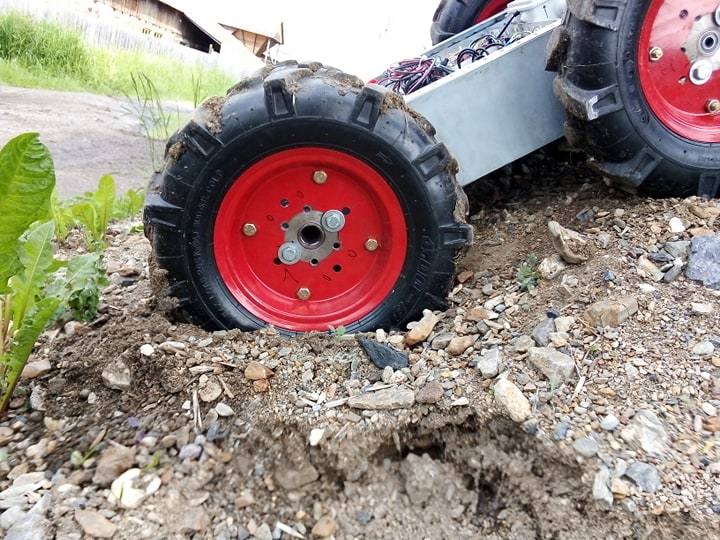
\includegraphics[width=.5\linewidth]{Meresek/Mozgasok/HomokosDomb/kep1.jpg}\hfill
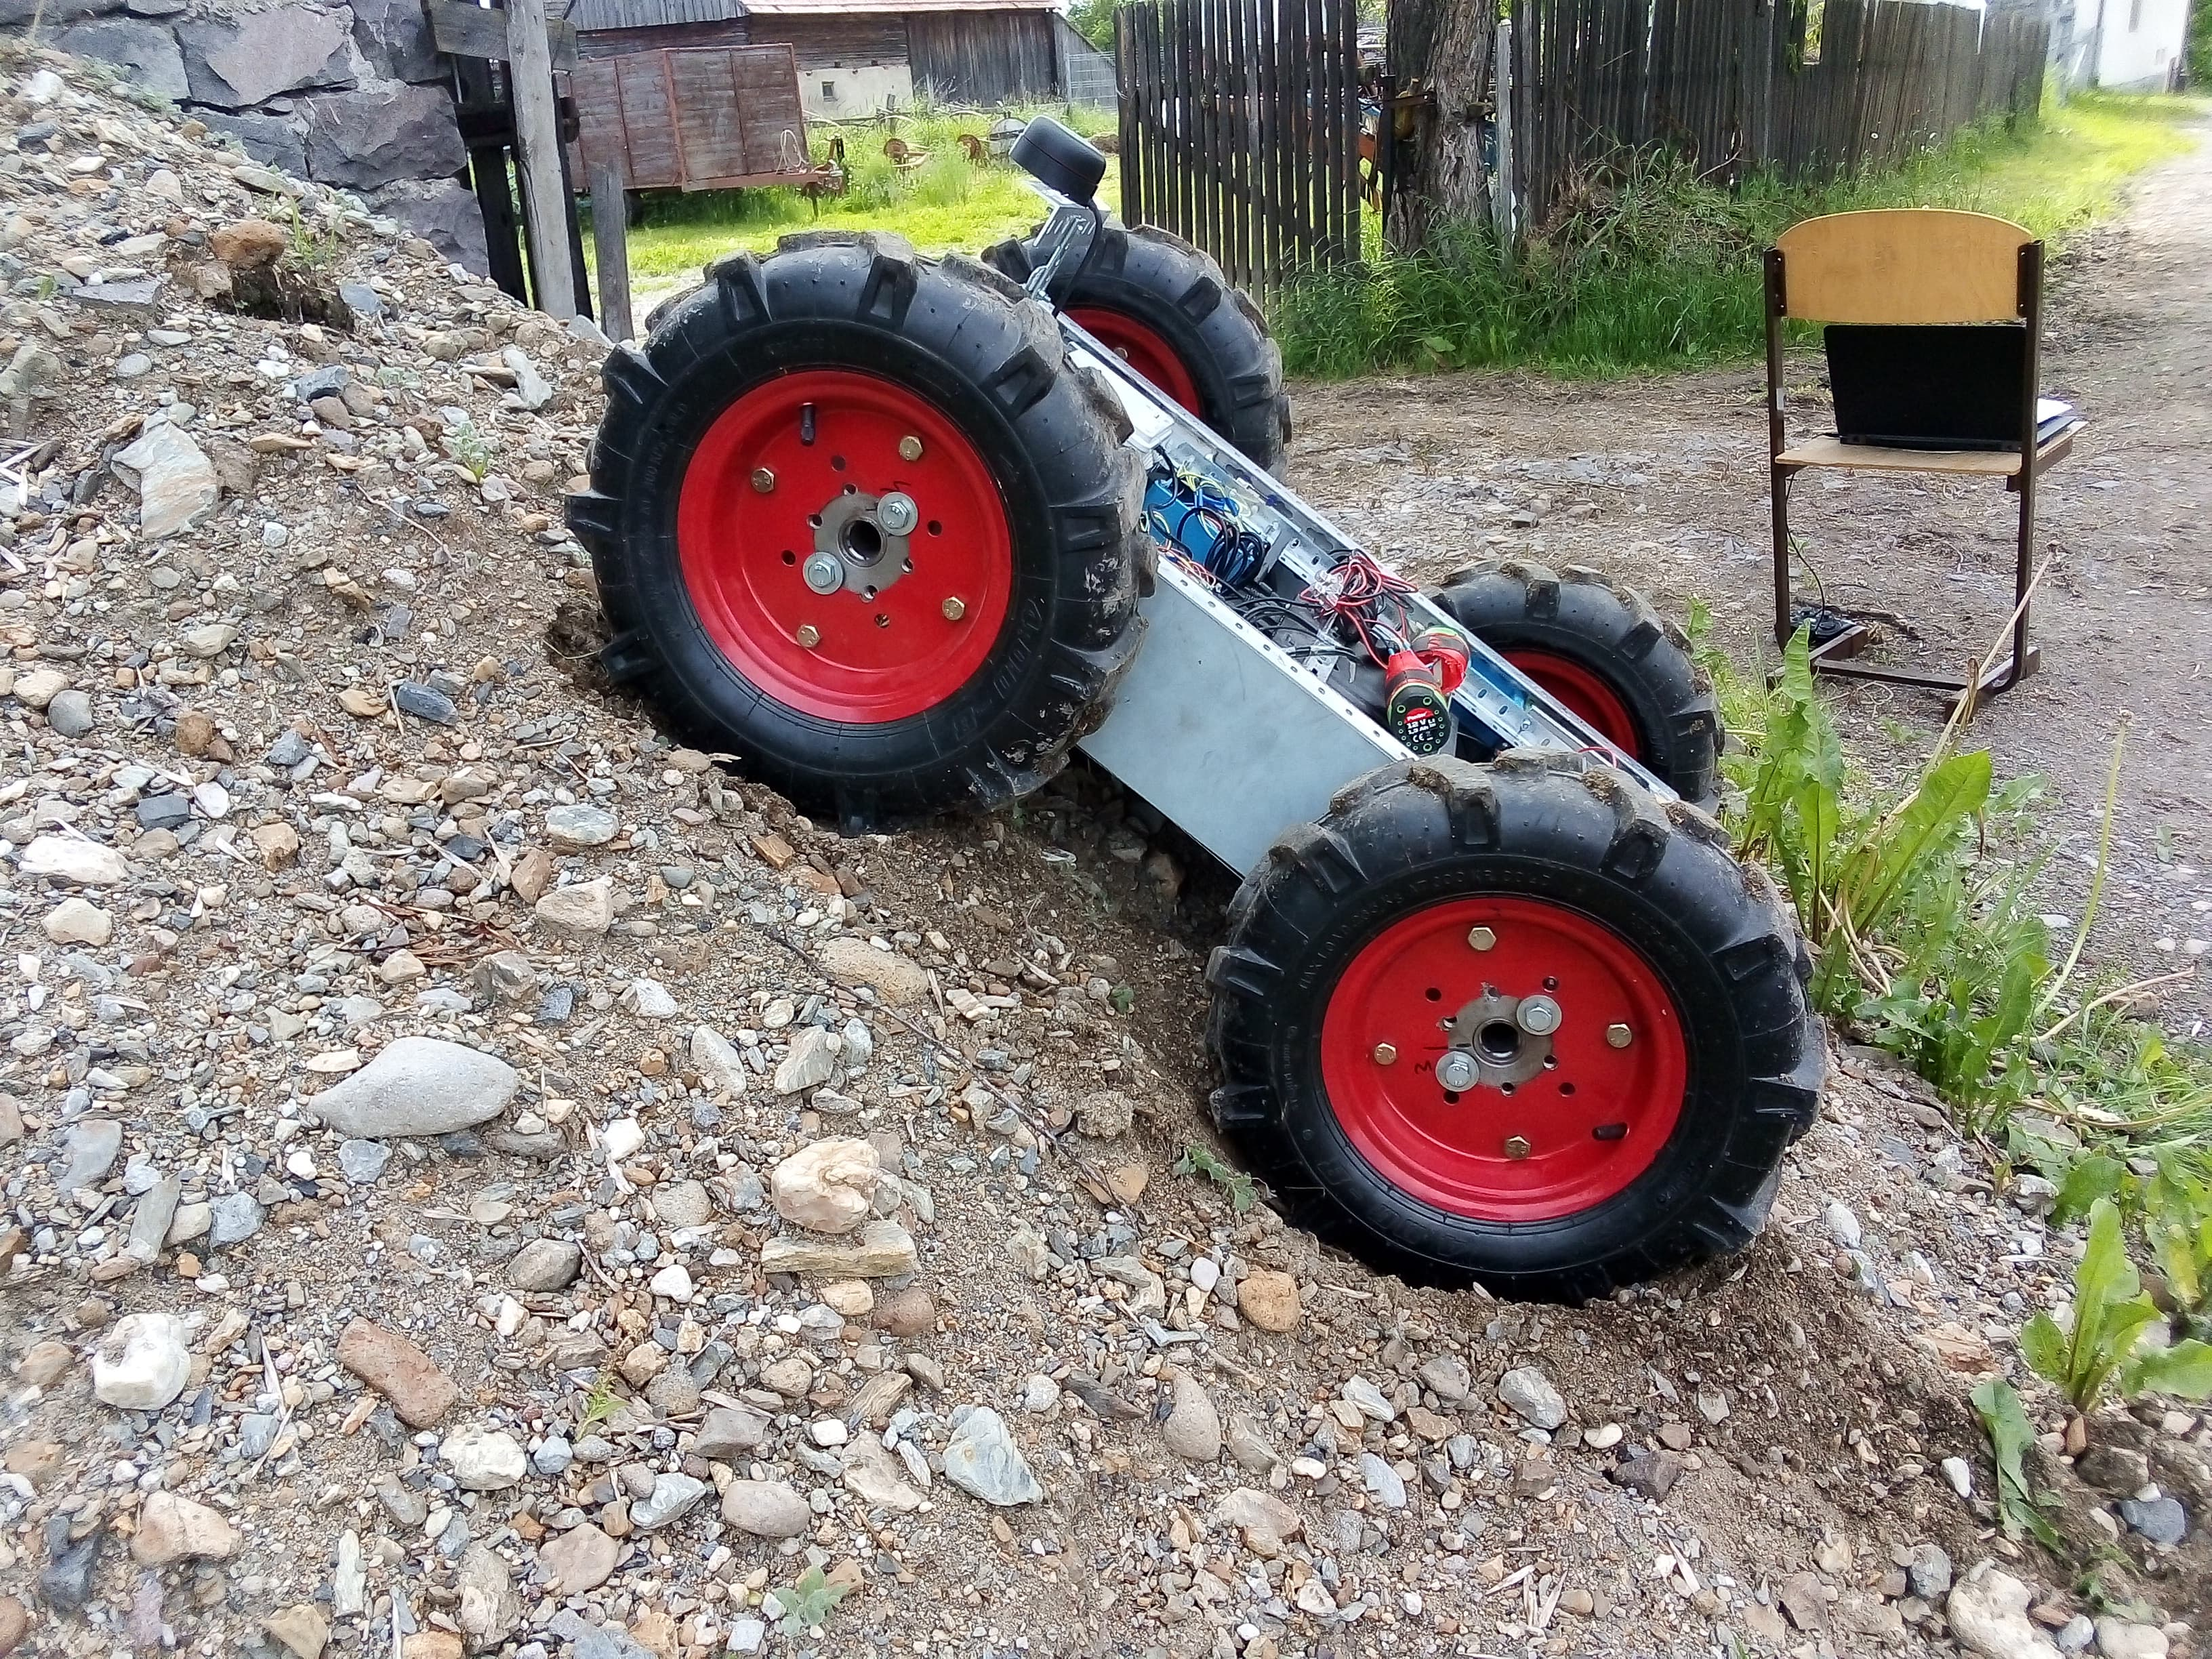
\includegraphics[width=.5\linewidth]{Meresek/Mozgasok/HomokosDomb/kep2.jpg}
\caption{Homokbat sülyet kerek 45\degree lejtön, 10 cm mélyen,elakadt robot a lejtőn 0.5m megtett ut után}
\label{fig:Hlejto1}
\end{figure}






\begin{figure}[H]
  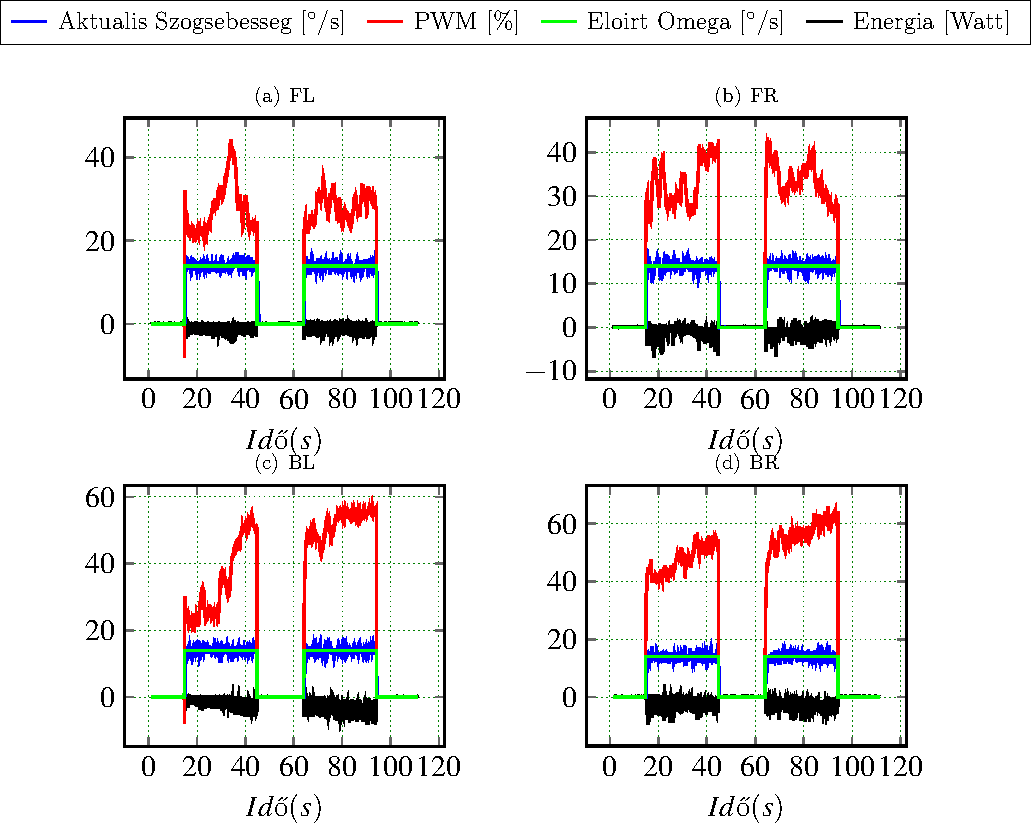
\includegraphics{tikz/HlejtoKerek.pdf}
  \caption{}
  \label{fig:HlejtoKerek}
\end{figure}













\subsection{Lepcson}




\renewcommand{\GlobalPath}{Meresek/Mozgasok/Lepcso}
\renewcommand{\secondImage}{*} 

%kep a talajrol
%

\renewcommand{\sources}{}
\renewcommand{\captionn}{Kep a felszinrol}
\renewcommand{\figlabel}{figm}


\begin{kep}
    \begin{figure}[H]%
    \begin{center}
    
    \subfloat[label a]{
        {\includegraphics[width=9cm]{\mand{\GlobalPath}{talaj1.jpg}} }
        \label{fig:ex3-a}
    }%
    
    \ifthenelse{\equal{\secondImage}{*}}
    {}
    {
        \qquad
        \subfloat[label b]{{\includegraphics[width=9cm]{\mand{\GlobalPath}{talaj1.jpg}} }}%
    }
  
    \label{fig:example}%
    \end{center}
\end{figure}
\end{kep}

\renewcommand{\secondImage}{*}



%1
% %1
    \begin{figure}
    
        %-------------------------------------------------Joint Adatok---------------
        \begin{subfigure}{\textwidth}
            \begin{center}
        
            \input{\mand{\GlobalPath}{L.tex}}
            \pgfplotstableread{NodeLeft.dat}{\leftNode}

            
            \input{\mand{\GlobalPath}{R.tex}}
            \pgfplotstableread{NodeRight.dat}{\rightNode}

        
            \begin{tikzpicture}
            \pgfplotsset{every axis plot/.append style={very thick}}
            \setcaptionsubtype
            
            % megjelenites beallitasai
            
            \begin{groupplot}[%
                        ,group style={%
                            ,group name=my plots
                            ,group size=2 by 2
                            ,vertical sep=1.8cm,
                            ,horizontal sep = 2.4cm,
                            ,ylabels at=edge left
                        }
                        ,width=7cm
                        ,height=6cm
                        ,try min ticks=5
                        ,xlabel={\bfseries{\emph{\idoFelirat}}}
                        ,zlabel={\bfseries{\emph{kg}}}
                        %%ha kell y felirat az elso ketore
                        %,ylabel={\bfseries{\degree$/s$}}
                        %,ylabel style={rotate=-90}
                        %,xtick={0,10,...,60},
                        %,minor tick num=5
                        %,xtick distance=10
                        %,ytick distance=25
                        ,grid=major%both
                        ,every both grid/.style={gray, opacity=0.7},
                        view={0}{90},
                        legend columns=2,
                        %xmin=0,xmax=0.65,
                        %ymin=0,ymax=0.65,
                       % zmin=-5,zmax=60,
                        ]
            %% ide jonnek a adatok. 
            
            %ha kell felirat be kell teni a nextplot[] parameterei koze
            % \nextgroupplot[ylabel=\degree$/s$, ylabel style={rotate=-90},legend to name={CommonLegend},legend style={legend columns=2}]
            \nextgroupplot[]
                \addplot [color=green,each nth point={\nth}] table [header=true, x=Time, y=refOmegaA] {\leftNode};\label{plots:plot3}
                \addplot [color=black,each nth point={\nth}] table [header=true, x=Time, y=effortA] {\leftNode};\label{plots:plot4}
                \addplot [color=blue,each nth point={\nth}] table [header=true, x=Time, y=omegaA] {\leftNode}; \label{plots:plot1}
                \addplot [color=red,each nth point={\nth}] table [header=true, x=Time, y=pwmA] {\leftNode};\label{plots:plot2}
                \coordinate (top) at (rel axis cs:0,1);% coordinate at top of the first plot
            
            \nextgroupplot[]
                \addplot [color=green,each nth point={\nth}] table [header=true, x=Time, y=refOmegaA] {\rightNode};
                \addplot [color=black,each nth point={\nth}] table [header=true, x=Time, y=effortA] {\rightNode};
                \addplot [color=blue,each nth point={\nth}] table [header=true, x=Time, y=omegaA] {\rightNode};
                \addplot [color=red,each nth point={\nth}] table [header=true, x=Time, y=pwmA] {\rightNode};
                    
            \nextgroupplot[]
                \addplot [color=green,each nth point={\nth}] table [header=true, x=Time, y=refOmegaB] {\leftNode};
                \addplot [color=black,each nth point={\nth}] table [header=true, x=Time, y=effortB] {\leftNode};
                \addplot [color=blue,each nth point={\nth}] table [header=true, x=Time, y=omegaB] {\leftNode};
                \addplot [color=red,each nth point={\nth}] table [header=true, x=Time, y=pwmB] {\leftNode};
                   
            \nextgroupplot[]
                \addplot [color=green,each nth point={\nth}] table [header=true, x=Time, y=refOmegaB] {\rightNode};
                \addplot [color=black,each nth point={\nth}] table [header=true, x=Time, y=effortB] {\rightNode};
                \addplot [color=blue,each nth point={\nth}] table [header=true, x=Time, y=omegaB] {\rightNode};
                \addplot [color=red,each nth point={\nth}] table [header=true, x=Time, y=pwmB] {\rightNode};
                \coordinate (bot) at (rel axis cs:1,0);% coordinate at bottom of the last plot
            \end{groupplot}
            
            %\path [nodes={anchor=south,rotate=90,font=\large\bfseries,midway}]
            %  (my plots c1r1.outer north west)--(my plots c1r2.outer south west)
            %    node {Testing of Parameters 1}
            %  (my plots c2r1.outer north west)--(my plots c2r2.outer south west)
            %    node {Testing of Parameters 2};
            
            % legend
            \node[text width=.5\linewidth,align=center,anchor=south] at (my plots c1r1.north) {\caption[]{FL\label{subplot:one}}};
            \node[text width=.5\linewidth,align=center,anchor=south] at (my plots c2r1.north) {\caption[]{FR\label{subplot:two}}};
            \node[text width=.5\linewidth,align=center,anchor=south] at (my plots c1r2.north) {\caption[]{BL\label{subplot:three}}};
            \node[text width=.5\linewidth,align=center,anchor=south] at (my plots c2r2.north) {\caption[]{BR\label{subplot:four}}};
            
            %\path (top-|current bounding box.west)-- 
            %      node[anchor=south,rotate=90] {throughput} 
            %      (bot-|current bounding box.west);
            % legend
            \path (top|-current bounding box.north)--
                  coordinate(legendpos)
                  (bot|-current bounding box.north);
            \matrix[
                matrix of nodes,
                anchor=south,
                draw,
                inner sep=0.2em,
                draw
              ]at([yshift=1ex]legendpos)
              {
                \ref{plots:plot1}& Aktualis Szogsebesseg [\degree$/s$]&[5pt]
                \ref{plots:plot2}& PWM [$\%$] &[5pt]
                \ref{plots:plot3}& Eloirt Omega [\degree$/s]$
                \ref{plots:plot4}& Energia $[Watt]$ &[5pt]\\
            };
           % \centering
            \end{tikzpicture}
            \end{center}
        \end{subfigure}
        
        \iffalse
        %-------------------------------------------------Power Adatok---------------
        \newline
        \begin{subfigure}{\textwidth}
        \begin{center}
        \input{\mand{\GlobalPath}{Power.tex}}
        \pgfplotstableread{Power.dat}{\power}
        
        
        \begin{tikzpicture}
        \pgfplotsset{every axis plot/.append style={very thick}}
        \setcaptionsubtype
        
        % megjelenites beallitasai
        
        \begin{groupplot}[%
                    ,group style={%
                        ,group name=my plots
                        ,group size=1 by 1
                        ,vertical sep=2cm,
                        ,horizontal sep = 0cm,
                        ,ylabels at=edge left
                    }
                    ,width=14.5cm
                    ,height=6cm
                    ,try min ticks=5
                    ,xlabel={\bfseries{\emph{\idoFelirat}}}
                    %,ylabel={\bfseries{\emph{A}}}
                    %,zlabel={\bfseries{\emph{kg}}}
                    ,grid=both
                    ,every both grid/.style={gray, opacity=0.5}
                    ,view={0}{90},
                    %,xtick distance=10
                    %,minor tick num=5
                    %,ytick distance=5
                    %xmin=0,xmax=0.65,
                    %ymin=0,ymax=0.65,
                    %zmin=-5,zmax=60,
                    ]
        %% ide jonnek a adatok.            
                    
        \nextgroupplot[ylabel=\emph{}, ylabel style={rotate=-90}]
         \addplot [color=red,each nth point={\nth}] table [header=true, x=Time, y=voltage] {\power};\label{plots:plot11}
         \addplot [color=green,each nth point={\nth}] table [header=true, x=Time, y=current]{\power};\label{plots:plot12}
         \addplot [color=black,each nth point={\nth}] table [header=true, x=Time, y=power] {\power};\label{plots:plot13}
        \end{groupplot}
        
        %\path [nodes={anchor=south,rotate=90,font=\large\bfseries,midway}]
        %  (my plots c1r1.outer north west)--(my plots c1r2.outer south west)
        %    node {Testing of Parameters 1}
        %  (my plots c2r1.outer north west)--(my plots c2r2.outer south west)
        %    node {Testing of Parameters 2};
        
        % legend
        \node[text width=.5\linewidth,align=center,anchor=south] at (my plots c1r1.north) {\caption[]{Energia Fogyasztas\label{subplot:one}}};
        
        %\path (top-|current bounding box.west)-- 
            %      node[anchor=south,rotate=90] {throughput} 
            %      (bot-|current bounding box.west);
            % legend
            \path (top|-current bounding box.north)--
                  coordinate(legendpos)
                  (bot|-current bounding box.north);
            \matrix[
                matrix of nodes,
                anchor=south,
                draw,
                inner sep=0.2em,
                draw
              ]at([yshift=1ex]legendpos)
              {
                \ref{plots:plot11}&  Akumlator Feszultsege [V]&[5pt]
                \ref{plots:plot12}& Akkumlator Arama [A] &[5pt]
                \ref{plots:plot13}& Teljesitmeny [W] \\
            };
        
        %\centering
        \end{tikzpicture}
        \end{center}
        \end{subfigure}
        % Caption
        %\caption[]{$SSMR-4W$ tipusu robot kereknyomoerok kerekenkeni változása a sulypont fuggvenyeben}\label{abserror}
        \fi
    \end{figure}


A kovetkező méresek soran a robot egy 40 \degree lepcson lefele és felfele is mozog a lepcsőre merőleges irányban. A robot viselkedése a mozgás során, lefele könyeden megy gond nélkül, felfele viszont a kerekek a következő lépcsöfok élléről lecsusza viszaesnek.

A \ref{fig:LepcsoLexx} latható amit a lépcsőn lefele, a mozgato motrok mért értékei. és a \ref{fig:LepcsoFelxx} viszafele mozgás során a mért értékek. A beavatkozó jel nagysága 10\% -al  nagyobb viszafele mozgas során. A mérések elvegzésekor a hajtást végző motrok a kisebbik átételfokozatban voltak, igy nagyobb forgatónyomatékot adtak le.

\begin{figure}[H]
  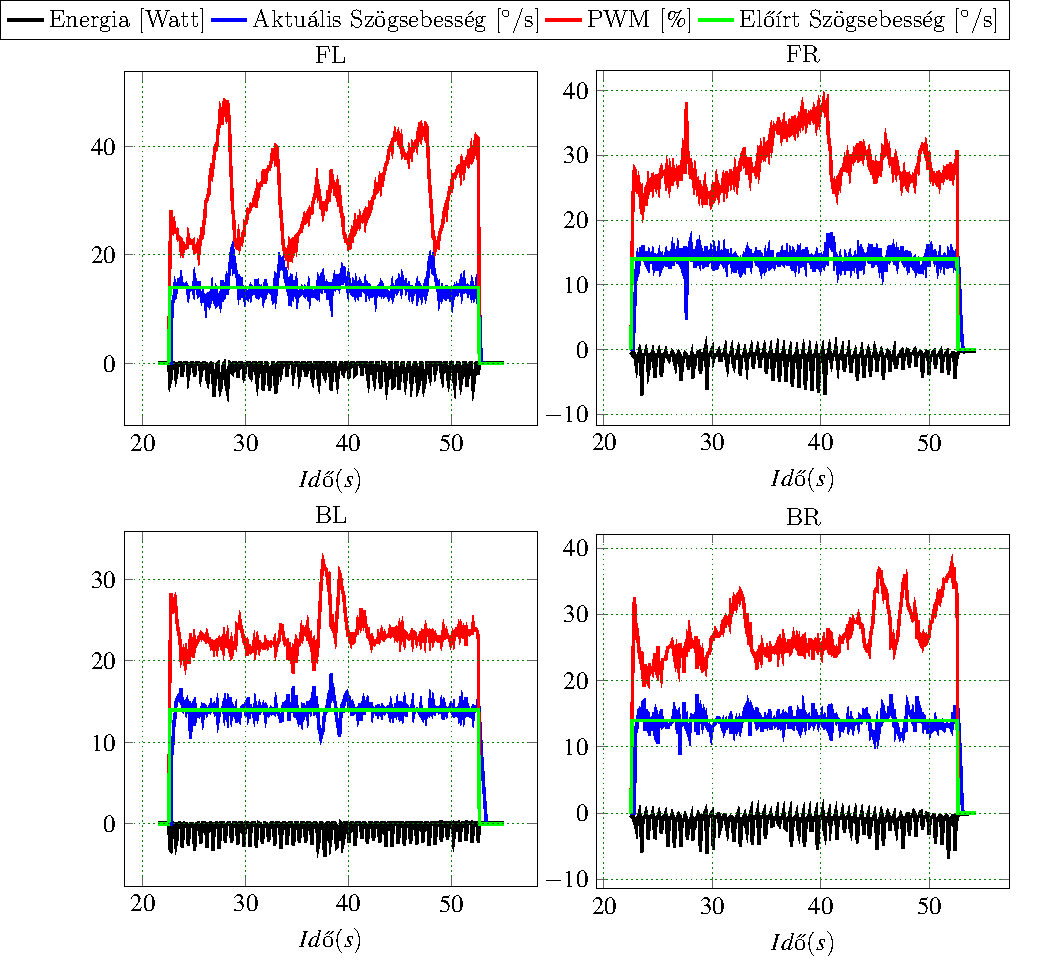
\includegraphics{tikz/LepcsoLexx.pdf}
  \caption{Lépcsőn lefele mozgás.}
  \label{fig:LepcsoLexx}
\end{figure}

A roboton IMU szenzora által mért értékek mutatjak amint a $g=9.81 m/s^2$ gravitácios gyorsulás megjelenik a $aZ$ tengelyen \ref{fig:ImuLepcsoLe1}. Kezdetben a robot vizszinteshez közeli állapotban van X és Y.  A lépcson lefele mozgás során a $g$ fokoatosan átevődik az $aX$ tengelyre is amiat, hogy a robot előre dől. A robot három lépcsofokon halad át ami látható az ábrán is.

\begin{figure}[H]
  \begin{center}
  	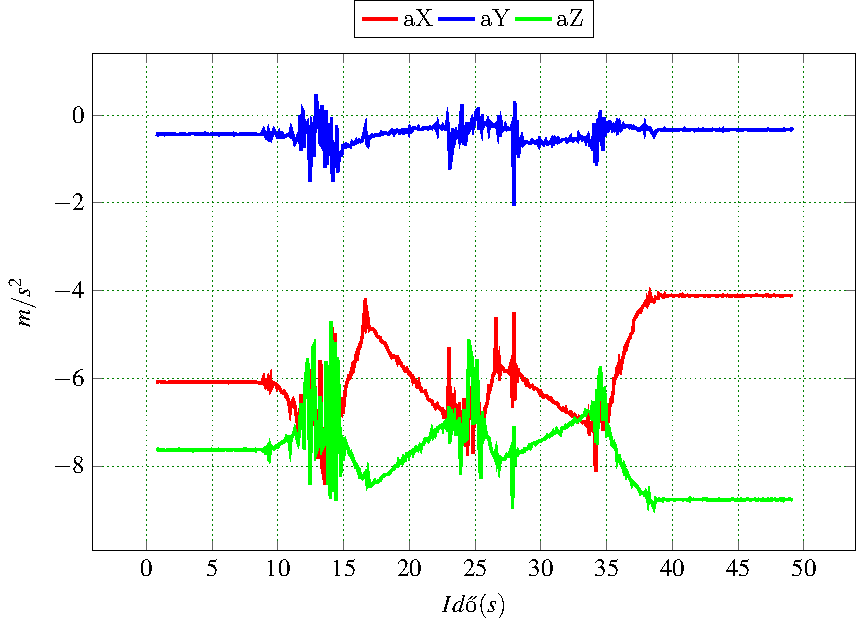
\includegraphics[scale=0.8]{tikz/ImuLepcsoLe1.pdf}
  \end{center}
  \caption{Lépcsön lefele mozgás, három lépcsőfok.}
  \label{fig:ImuLepcsoLe1}
\end{figure}

\begin{figure}[H]
  \begin{center}
  	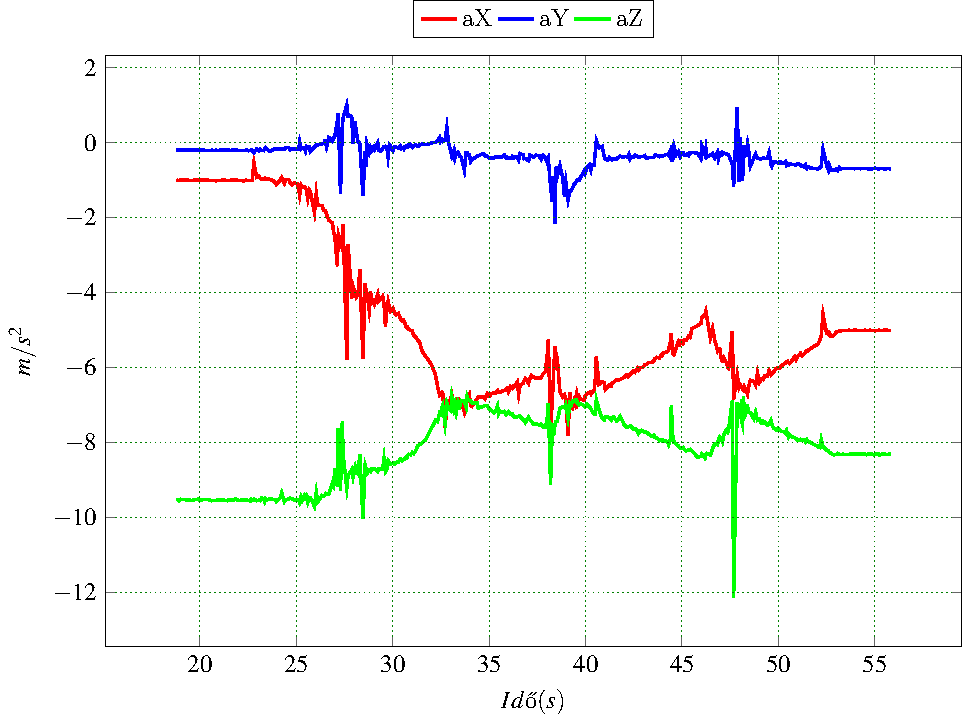
\includegraphics[scale=0.8]{tikz/ImuLepcsoFel1.pdf}
  \end{center}
  \caption{Lépcsőn felfele mozgás, kétlépcsőfok.}
  \label{fig:ImuLepcsoFel1}
\end{figure}

A lépcson felfele mozgás során a robot az eloző állapotból indul visszafele. Azokban a pillanatokban amikor a kerekek lecsusznak a lepcső éléről a kerekek szögsebessége megnő mert a surlodási erő lecsökken.  

Az \ref{fig:LepcsoFelxx} az $FL$ és $FR$ kerekeken nagyobb beavatkozójel esik, amiatt hogy megnő a merőleges nyomoerő.

\begin{figure}[H]
  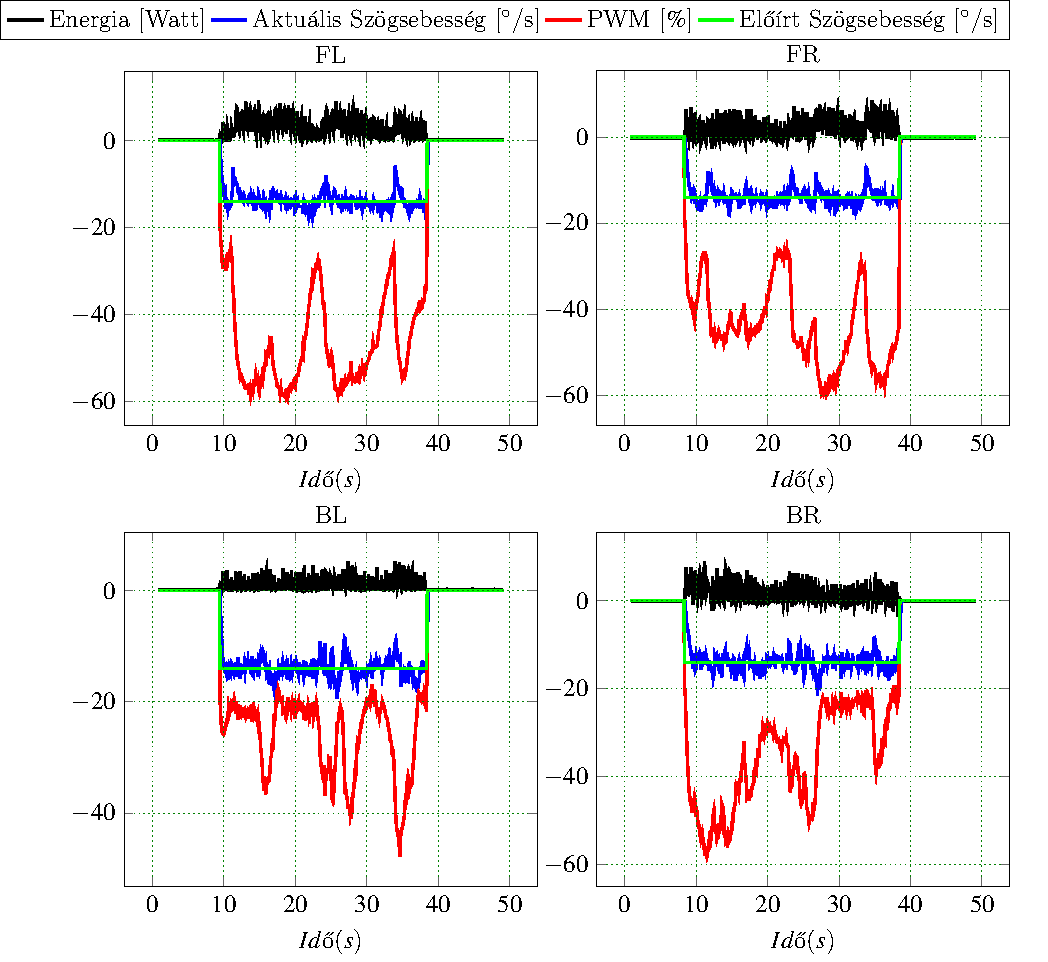
\includegraphics{tikz/LepcsoFelxx.pdf}
  \caption{Lépcsőn felfele mozgás}
  \label{fig:LepcsoFelxx}
\end{figure}

















\newpage

\subsection{Ismeretlen terep térképezése és robot lokalizálása (SLAM)}


\begin{figure}[H]
  \label{fig:hatsoudvarmap}
  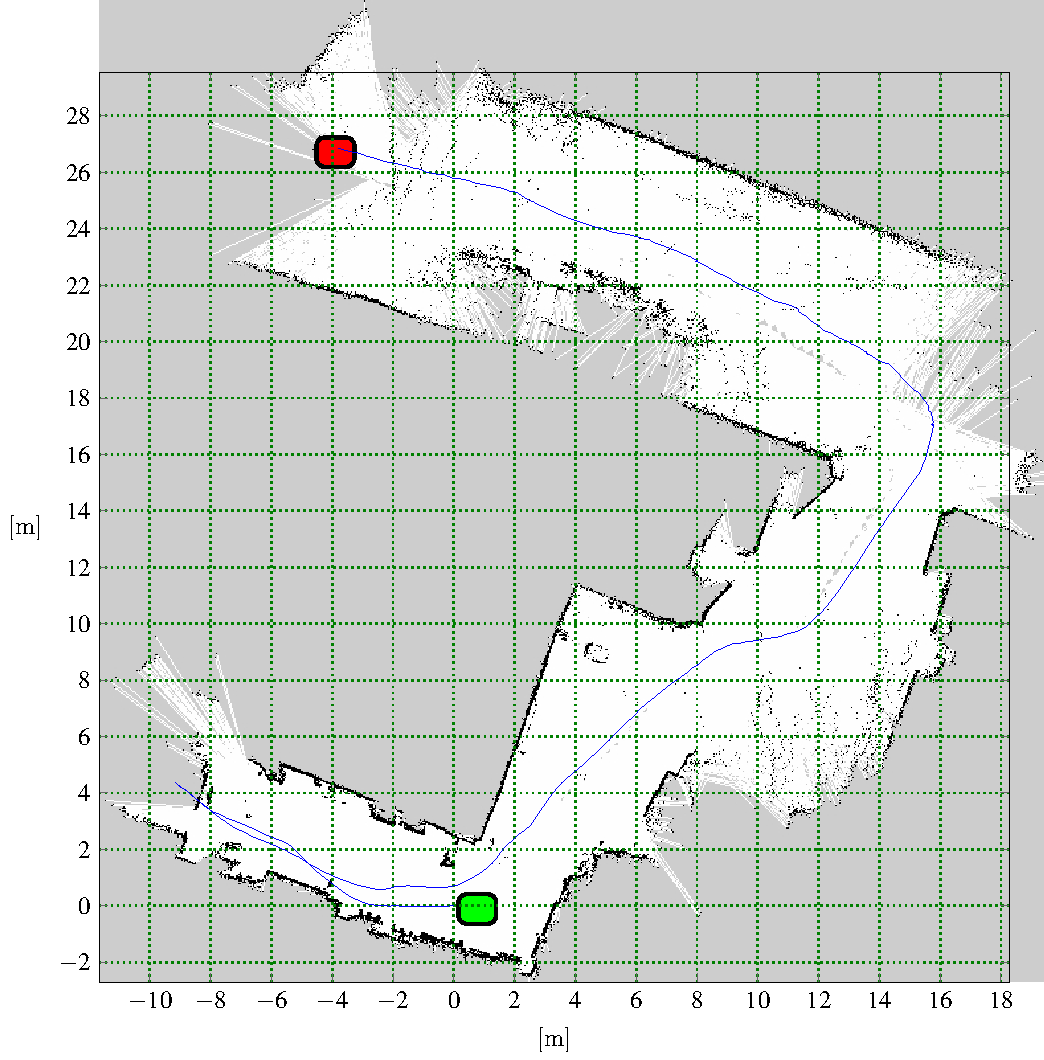
\includegraphics{tikz/hatsoudvarmap.pdf}
  \caption{Terkep keszitese mikozben taviranyitassal halad a robot.}
\end{figure}




